\documentclass[aspectratio=169]{beamer}

\title[Hubble tension]%(optional, only for long titles)
{Tensions in the Universe}
\subtitle{a crisis in precision cosmology?}
\date[2023-10-25] % (optional)
{25\textsuperscript{th} October 2023}

% Address
\author[Handley] % (optional, for multiple authors)
{Will Handley\\ \small{wh260@cam.ac.uk}}
\institute[University of Cambridge] % (optional)
{%
Astrophysics Department \\
Cavendish Laboratory\\
University of Cambridge
}

\institute[University of Cambridge] % (optional)
{%
    Gonville \& Caius College\\
    Kavli Institute for Cosmology, Cambridge
}

% Packages
\usepackage{graphicx}			% including images
\usepackage{color}			    % defining colors
\usepackage{multimedia}			% the sdss movie
\usepackage{xstring}			% for IfEqCase
\usepackage[overlay]{textpos}	% text positioning
\usepackage{textcomp}			% for euro symbol
\usepackage{pgfplots}  			% for graphs

\usepackage{tikz}			    % for tikz drawings
\usetikzlibrary{decorations.pathmorphing}
\usetikzlibrary{shapes,backgrounds}


% Colours


% Turn off the Navigation symbols
\beamertemplatenavigationsymbolsempty{}
%%%%%%%%%%%%%%%%%%%%%%%%%%%%%%% Colours %%%%%%%%%%%%%%%%%%%%%%%%%%%%%%%%%%%%%%

%%%%%%%%%%%%% the color scheme %%%%%%%%%%%%%%%%%%
                        						%
%% a light blue		                     		%
\definecolor{LightBlue}{RGB}{127,229,245}     	%
						                        %
%% a light grey					                %
\definecolor{LightGrey}{RGB}{250,250,250}	    %
						                        %
%% a darker grey			       	            %
\definecolor{DarkGrey}{RGB}{180,180,180}	    %
                                                %
%% the background				                %
\definecolor{BackgroundColor}{RGB}{0,0,0}	    %
						                        %
%%%%%%%%%%%%%%%%%%%%%%%%%%%%%%%%%%%%%%%%%%%%%%%%%

\setbeamercolor*{structure}{bg=BackgroundColor,fg=LightBlue}

% Background Colour
\setbeamercolor{background canvas}{bg=BackgroundColor}


% title for frames
%% a light blue
\setbeamercolor{frametitle}{fg=LightBlue,bg=BackgroundColor}
\setbeamerfont{frametitle}{series=\bfseries}

% subtitle for frames
%% a light grey
\setbeamercolor{framesubtitle}{fg=LightGrey,bg=BackgroundColor}

% text
%% a light grey
\setbeamercolor{normal text}{fg=LightGrey}

% items
%% a light blue
\setbeamercolor{item}{fg=LightBlue}

% title colors
%% a light blue
\setbeamercolor{section in toc}{fg=LightBlue}


%%%%%%%%%%%%%%% title page %%%%%%%%%%%%%%%%%%%%%%
\setbeamercolor{title}{fg=LightBlue,bg=BackgroundColor}
\setbeamercolor{subtitle}{fg=LightGrey,bg=BackgroundColor}
\setbeamercolor{author}{fg=LightBlue,bg=BackgroundColor}
\setbeamercolor{date}{fg=LightBlue,bg=BackgroundColor}
\setbeamercolor{institute}{fg=LightBlue,bg=BackgroundColor}
%%%%%%%%%%%%%%%%%%%%%%%%%%%%%%%%%%%%%%%%%%%%%%%%%

%\setbeamercolor{alerted text}{fg=C3}

\setbeamertemplate{blocks}[rounded]

\setbeamercolor{block body}{bg=BackgroundColor!80!LightBlue,fg=LightGrey}
\setbeamercolor{block title}{bg=BackgroundColor!60!LightBlue}
\setbeamerfont{block title}{series=\bfseries}

%\setbeamercolor{block title example}{fg=C2, bg=C2!15}
%\setbeamercolor{block body example}{bg=C2!5}

%\setbeamercolor{block title alerted}{fg=C3, bg=C3!15}
%\setbeamercolor{block body alerted}{bg=C3!5}







%%%%%%%%%%%%%%%%%%%%%%%%%%%%%%%%%%%%%%%%%%%%%%%%%%%%%%%%%%%%%%%%%%%%%%%%%%%%%%


% Environments
\usepackage{matplotlibcolors}
% Define an environment for a slide with a background image
\newenvironment{frameb}[2]
{	
	\IfEqCase{#1}{ 	% use the first argument to determine
			% whether to fit to height or to width
			%
	{h}		% fit to height
	{\usebackgroundtemplate{\includegraphics[height=\paperheight]{#2}}}
	{w}		% fit to width 
	{\usebackgroundtemplate{\includegraphics[width=\paperwidth]{#2}}}
			% error message:
	{\PackageError{frameb}{Undefined option to frameb: #1 first argument must either be h to stretch to height, or w to stretch to width}
	}}
	\begin{frame}   
}
{
	\end{frame}  
}

% Define an environment for a slide with a background image drawn by tikz
\newenvironment{framet}[3]
{	
% re-set the background... 
\setbeamertemplate{background}{
% ... as a TikZ box, with unitz re-scaled to 4:3 units
\begin{tikzpicture}[x=0.25\paperwidth,y=0.33333333\paperheight]
%
% If we want to put an image as well, then you should put:
\IfEqCase{#1}{
{h}    % Fit to height
{
\node[inner sep=0pt, anchor=south west] at (0,0) {\includegraphics[height=\paperheight]{#2}};
}
{w}    % Fit to width
{
\node[inner sep=0pt, anchor=north west] at (0,3) {\includegraphics[width=\paperwidth]{#2}};
}
{n}    % No background image
{}
{\PackageError{framet}{Undefined option to framet: #1 first argument must either be h to stretch to height, w to stretch to width, or n for no background image}
}
}
% Now the rest of the TikZ code
#3
%
% Finish the Tikz background
\end{tikzpicture}
%
}   % done setting the background
%
% Now begin the frame
	\begin{frame}   
}
{
% close off the frame
	\end{frame}  
}


%Tensions in the Universe: a crisis in precision cosmology?
%
%In 2013 the Planck satellite detailed in exquisite precision its measurements of the cosmic microwave background, and delivered an outstanding confirmation of our "standard model of the Universe", the so-called ΛCDM. However, since then observations using other cosmological phenomena such as supernovae and the patterns of galaxies have seemingly begun to derive different values of fundamental cosmological parameters, in "tension" with CMB observations.
%
%If true, such discrepancies are scientifically exciting. The last time this happened in the early 1990s, cosmologists were forced to introduce "Dark Energy" into our standard model. However, unlike three decades ago, after nearly five years of community effort, no satisfactory solution has been found.
%
%After introducing the core concepts (and common misconceptions) of modern cosmology, this talk will outline the current state of the art in precision measurements of the properties of our Universe, the discrepancies between different observations, and the open challenges in theoretically resolving them. On this tour we will encounter the current theories on the size, shape and contents of our universe, some of the largest and most complicated datasets ever collected, and the Bayesian inference and machine learning techniques required to analyse them.

%\includeonlyframes{current}


\begin{document}



\begin{frame}
  \titlepage{}
\end{frame}


\begin{frame}
    \frametitle{Modern Cosmology}
    \begin{columns}
        \column{0.77\textwidth}
        \begin{itemize}
            \item Precision answers to the oldest questions:
                \begin{itemize}
                    \item How old is the Universe? \only<2->{\hfill($13.8\pm0.1$ by)}
                    \item How did it begin? \only<3->{\hfill(Hot big bang)}
                    \item How will it end? \only<4->{\hfill(exponential expansion)}
                        \item What's its shape? \only<5->{\hfill(flat)}
                        \item How big is it \only<6->{\hfill(infinite, but only just)}
                        \item What's in it? \only<7->{\hfill($70\%$ dark energy, $25\%/5\%$ dark/visible matter)}
                \end{itemize}
                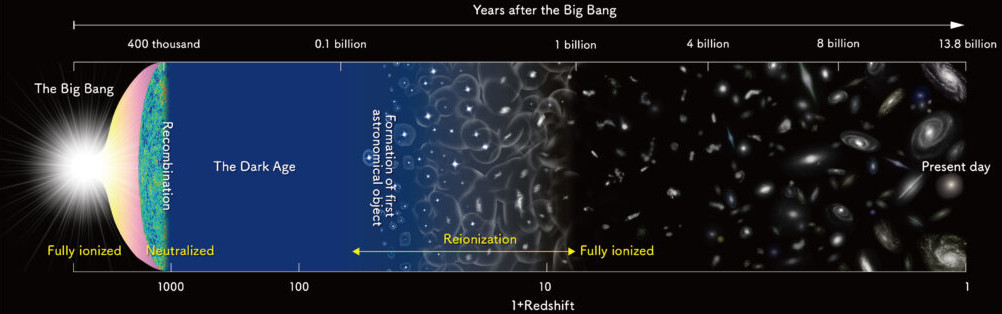
\includegraphics[width=\textwidth]{RAC/timeline-1024x369.jpg}
        \end{itemize}
        \column{0.23\textwidth}
        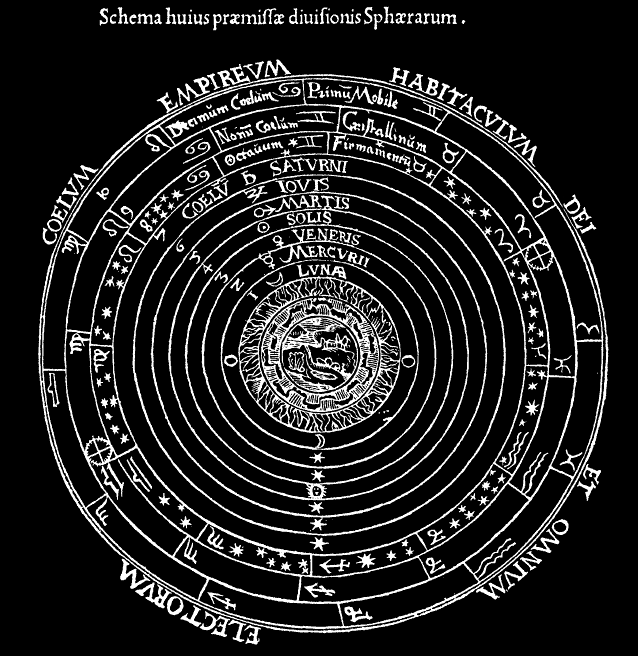
\includegraphics[width=\textwidth]{Images/Ptolemaicsystem-small-negate.png}
        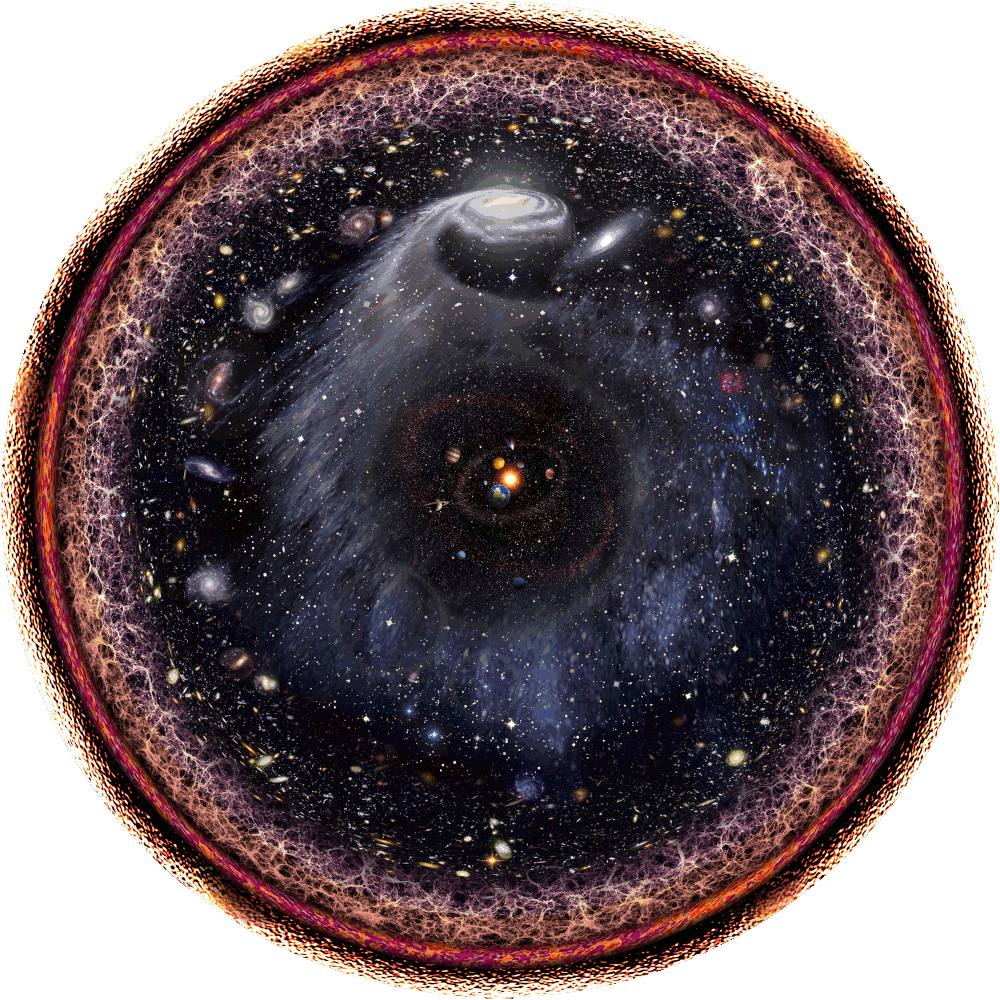
\includegraphics[width=\textwidth]{RAC/modern}
    \end{columns}
    \centerline{
    }
\end{frame}

\begin{frame}[label=why do cosmology]
    \frametitle{Why do cosmology?}
    \begin{columns}
        \column{0.3\textwidth}
        \begin{block}{Theory}
            Cosmology as a discipline requires understanding:
            \begin{itemize}
                \item General relativity
                \item Quantum mechanics
                \item Particle physics
                \item Thermodynamics
            \end{itemize}
            and how these interact in our evolving universal laboratory
        \end{block}
        
        \column{0.3\textwidth}
        \begin{block}{Observation}
            Over your career a suite of next generation instruments are due to come online:
            \begin{itemize}
                \item SKA, SO, JWST, ELT, LSST, Athena, e-ASTROGAM
                \item LIGO, Virgo, KAGRA, LISA, PTA
            \end{itemize}
        \end{block}

        \column{0.3\textwidth}
        \begin{block}{Inference}
            To join theory and observations requires innovation at the frontier of data analysis
            \begin{itemize}
                \item Bayesian inference
                \item Machine learning
                \item Artificial Intelligence
            \end{itemize}
        \end{block}
    \end{columns}
\end{frame}

\begin{frame}
    \frametitle{You are here}
    \begin{columns}
        \column{0.49\textwidth}
        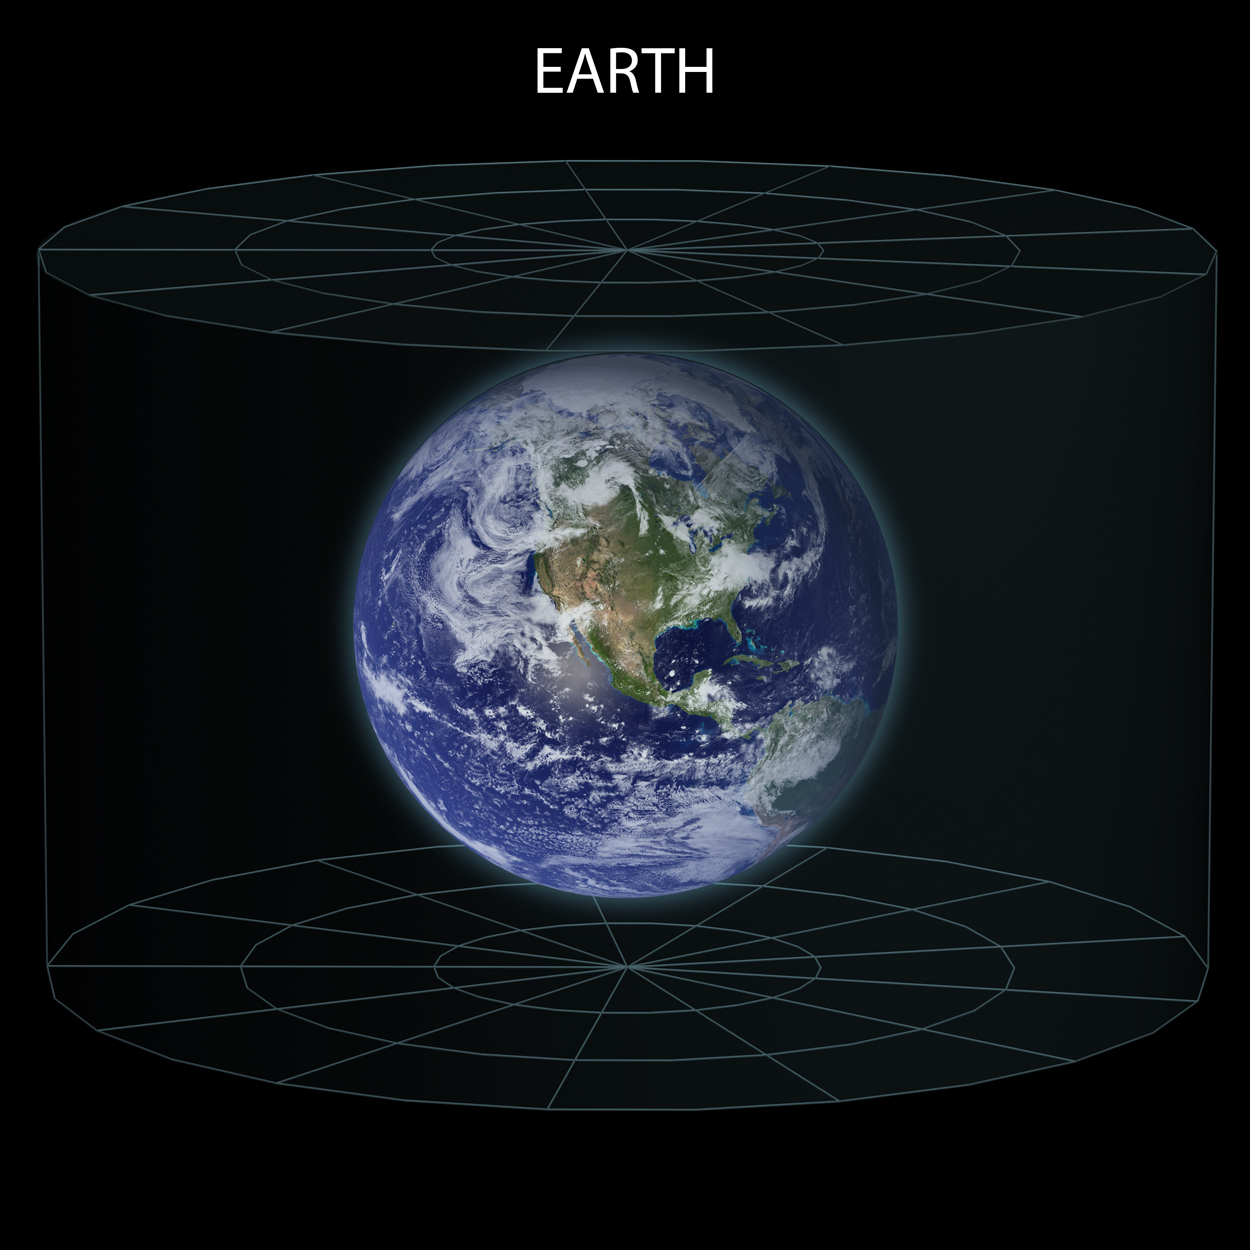
\includegraphics[width=\textwidth]{jwst/zoom_1.jpg}
        \column{0.49\textwidth}
    \end{columns}
\end{frame}

\begin{frame}
    \frametitle{You are here}
    \begin{columns}
        \column{0.49\textwidth}
        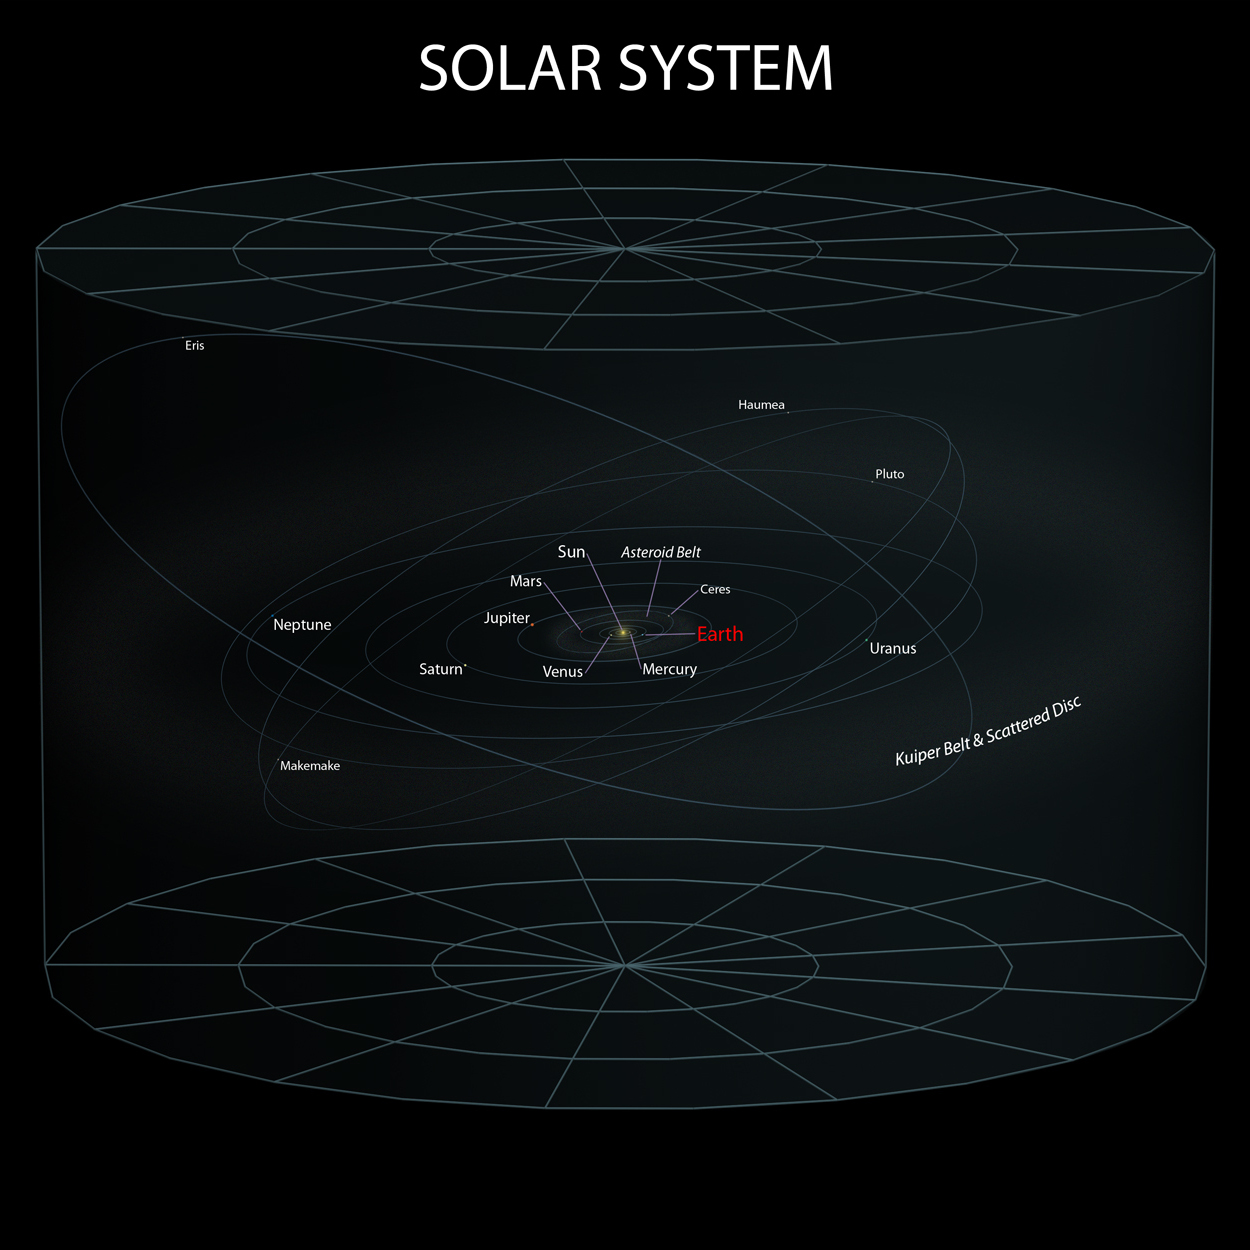
\includegraphics[width=\textwidth]{jwst/zoom_2.jpg}
        \column{0.49\textwidth}
        \begin{columns}
            \column{0.49\textwidth}
            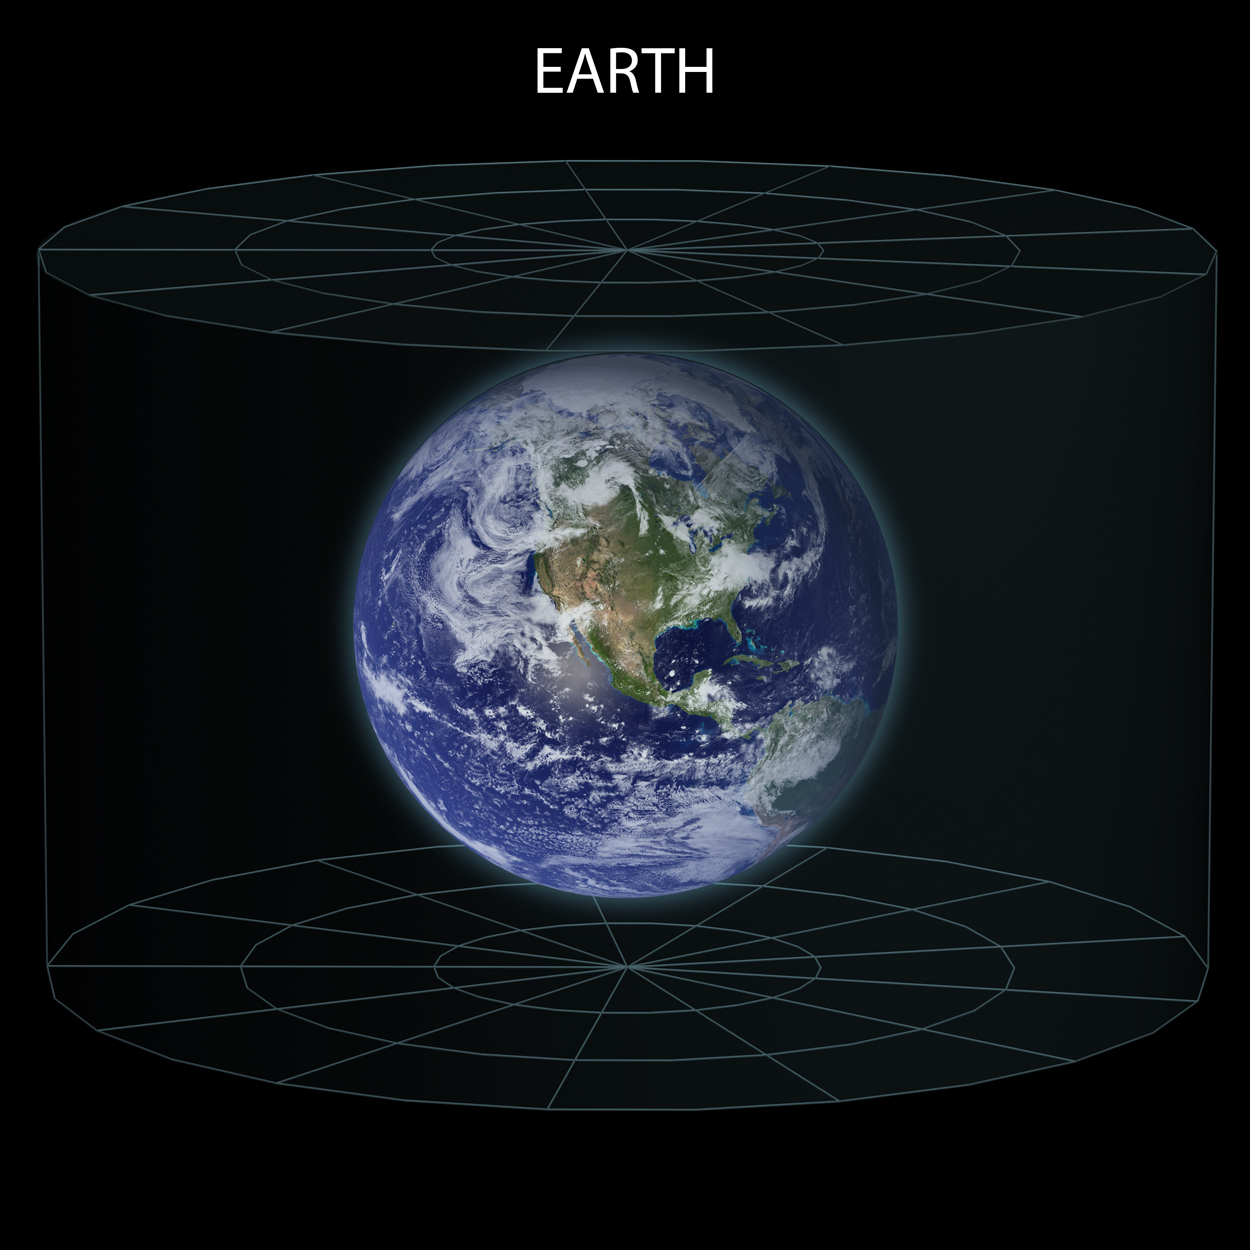
\includegraphics[width=\textwidth]{jwst/zoom_1.jpg}
            \column{0.49\textwidth}
        \end{columns}
    \end{columns}
\end{frame}

\begin{frame}
    \frametitle{You are here}
    \begin{columns}
        \column{0.49\textwidth}
        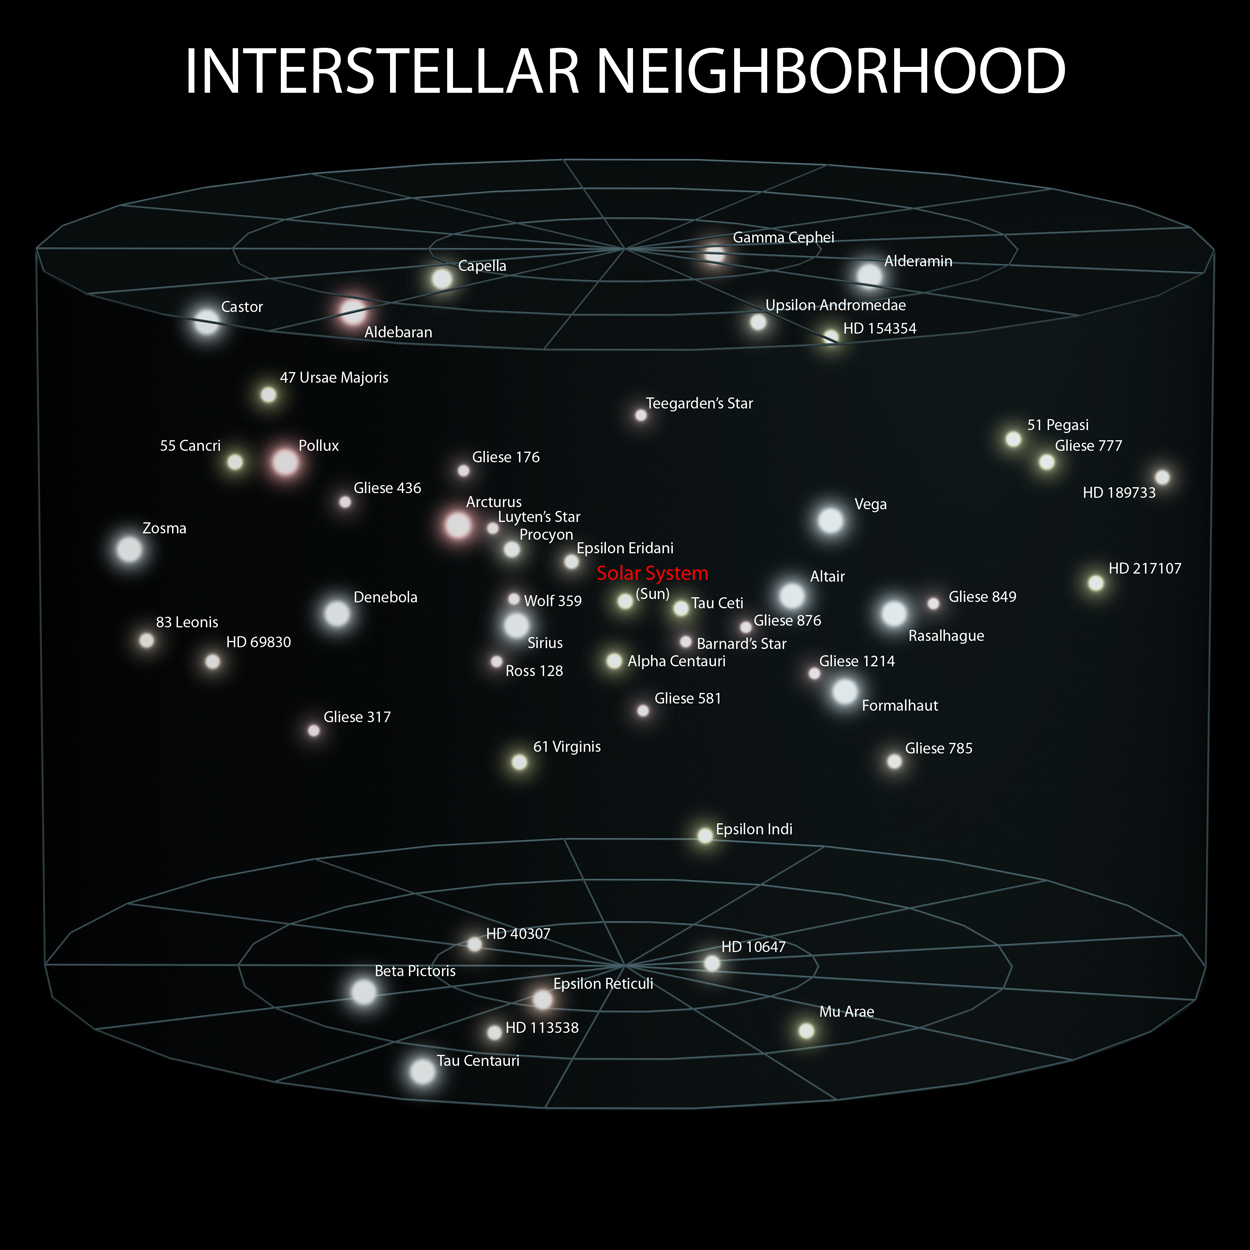
\includegraphics[width=\textwidth]{jwst/zoom_3.jpg}
        \column{0.49\textwidth}
        \begin{columns}
            \column{0.49\textwidth}
            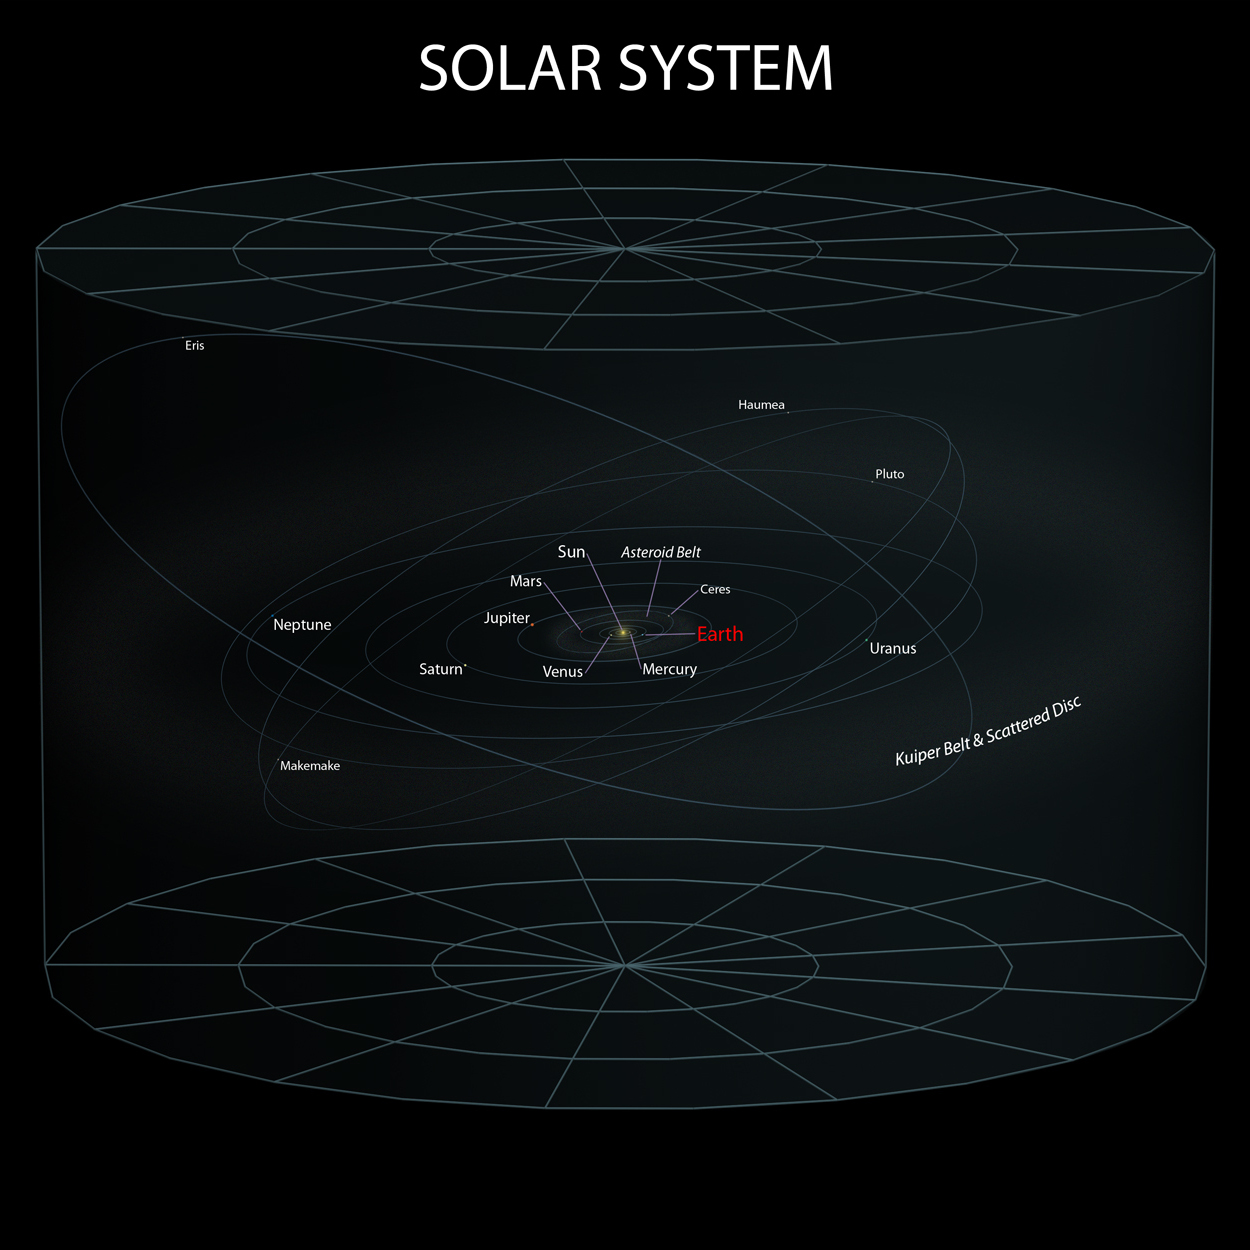
\includegraphics[width=\textwidth]{jwst/zoom_2.jpg}
            \column{0.49\textwidth}
            \begin{columns}
                \column{0.49\textwidth}
                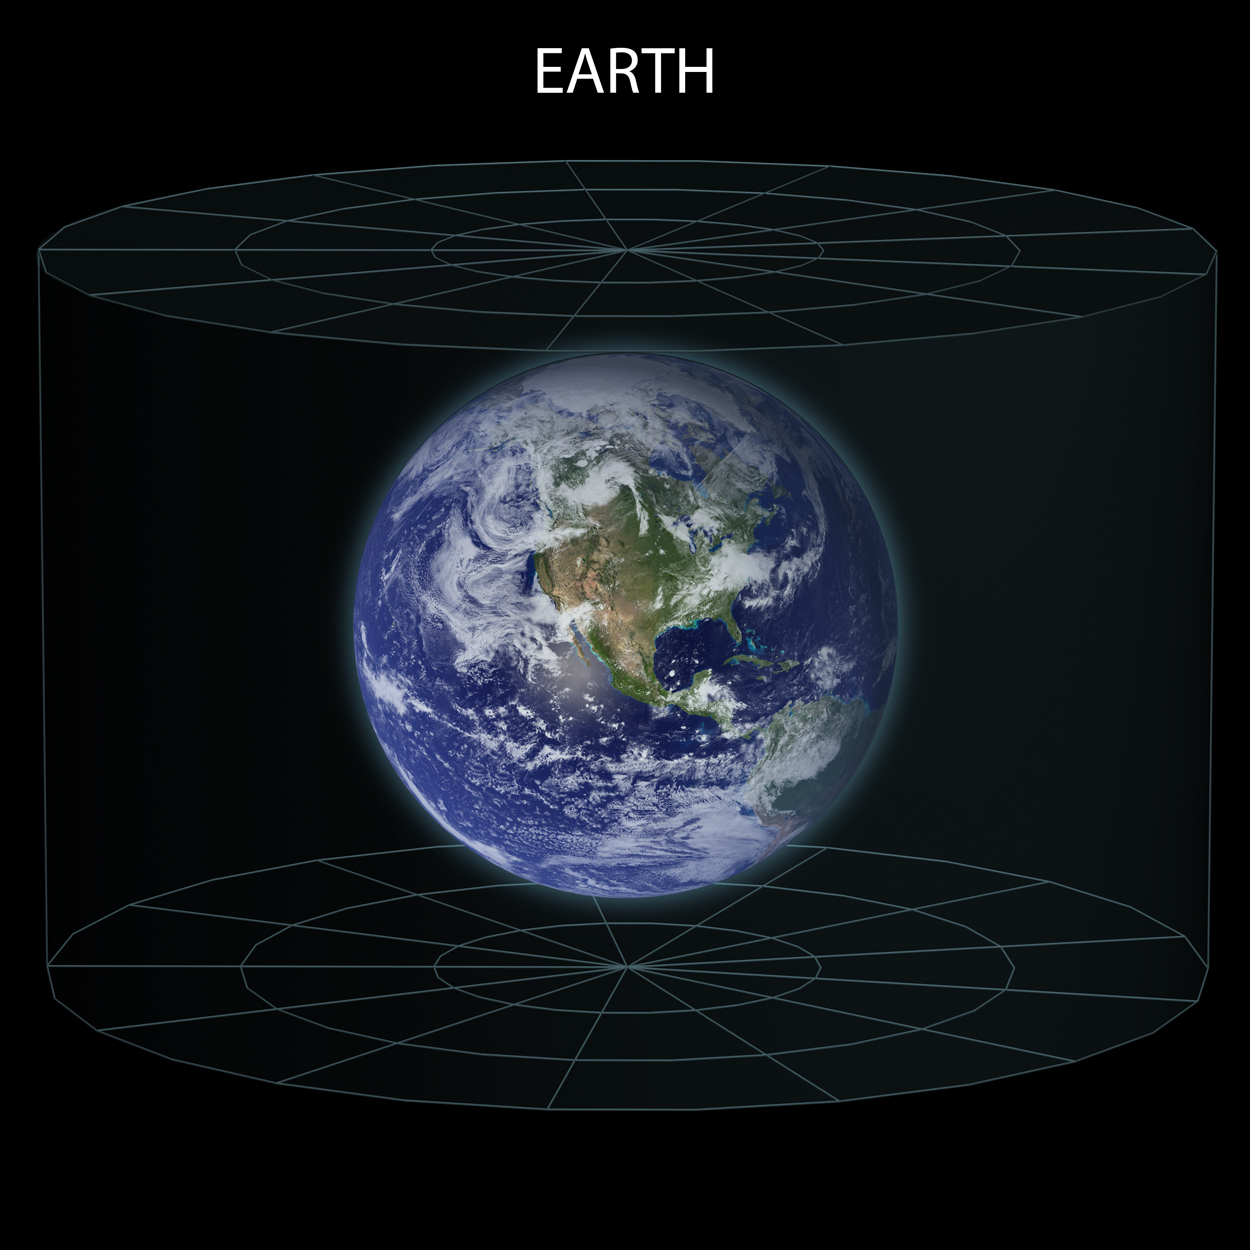
\includegraphics[width=\textwidth]{jwst/zoom_1.jpg}
                \column{0.49\textwidth}
            \end{columns}
        \end{columns}
    \end{columns}
\end{frame}

\begin{frame}
    \frametitle{You are here}
    \begin{columns}
        \column{0.49\textwidth}
        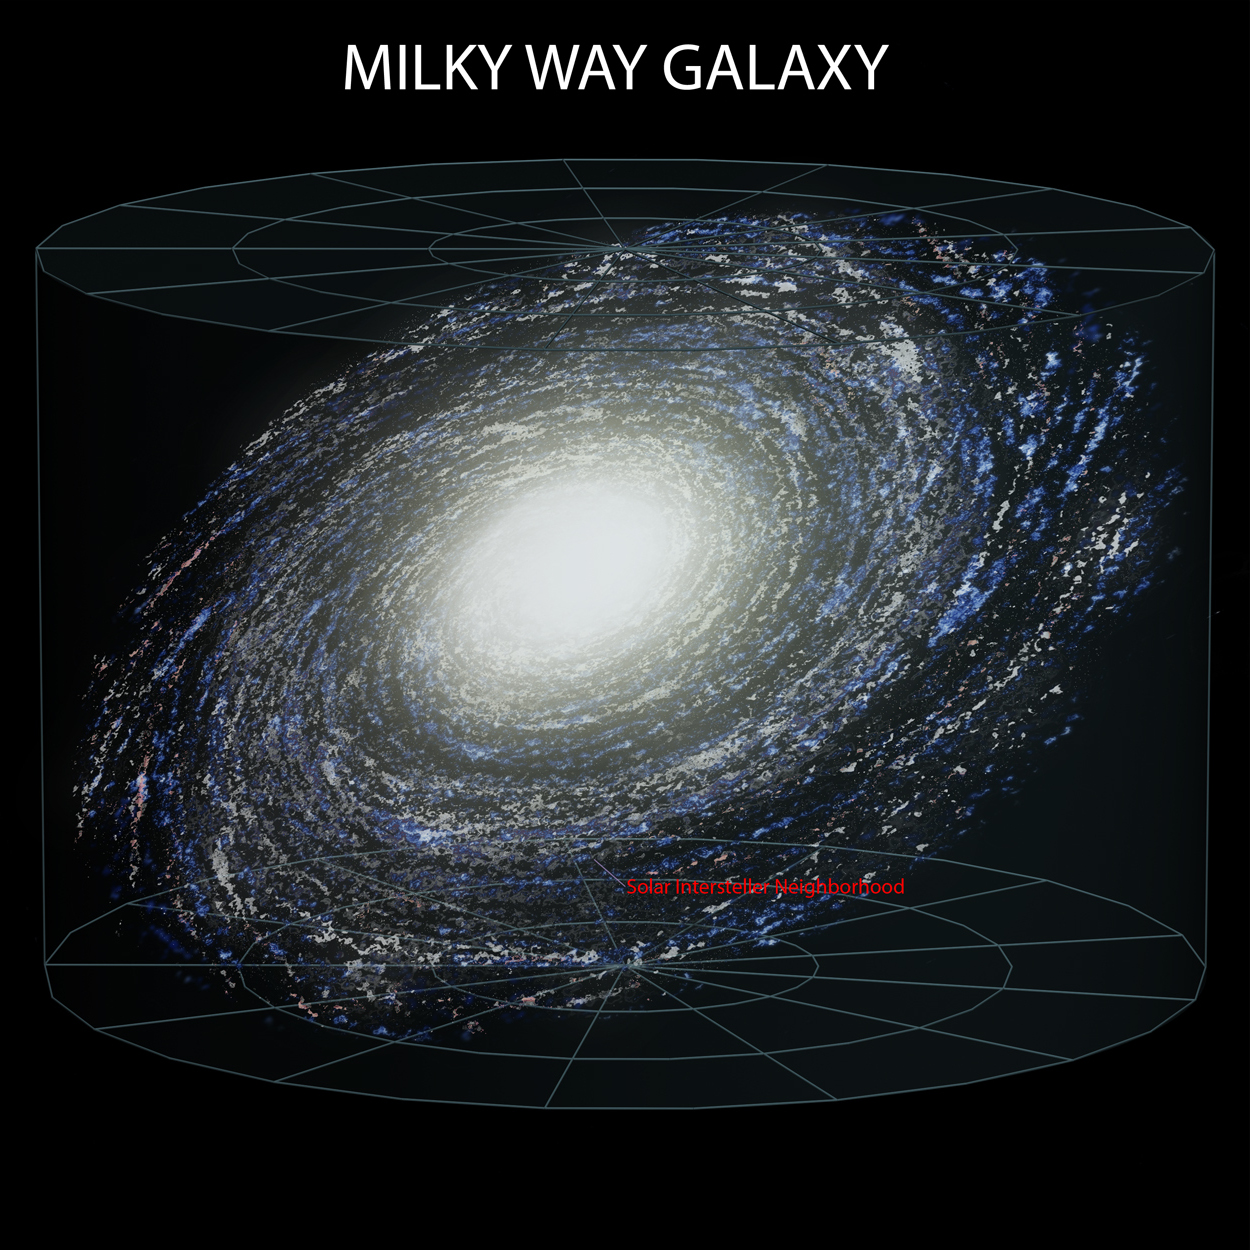
\includegraphics[width=\textwidth]{jwst/zoom_4.jpg}
        \column{0.49\textwidth}
        \begin{columns}
            \column{0.49\textwidth}
            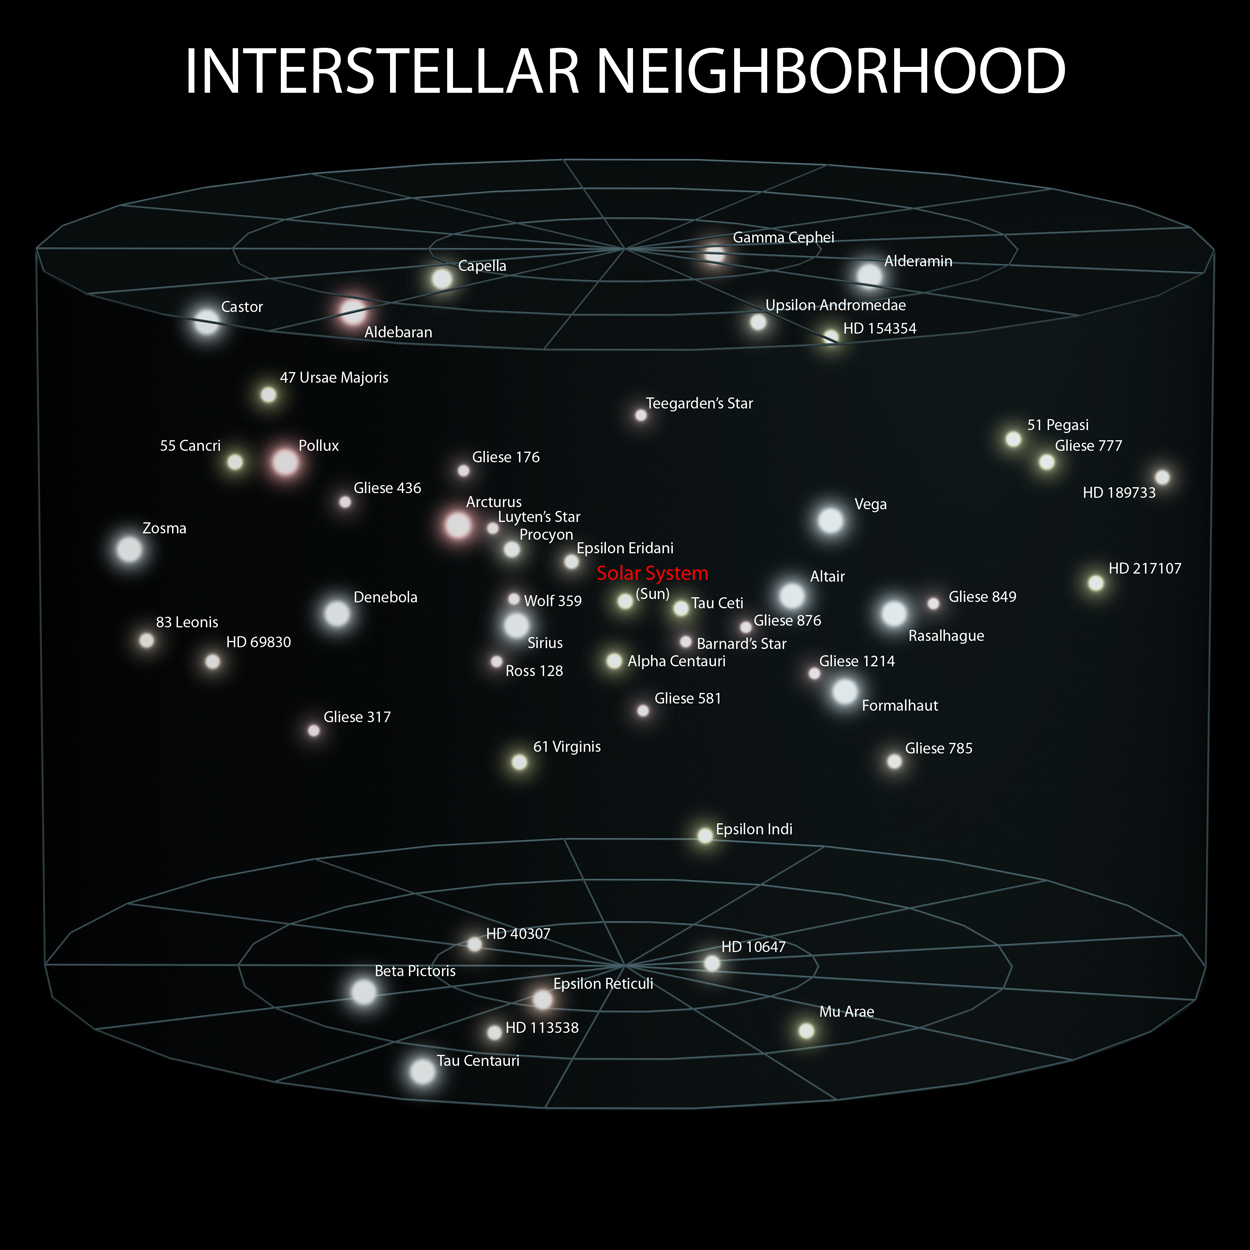
\includegraphics[width=\textwidth]{jwst/zoom_3.jpg}
            \column{0.49\textwidth}
            \begin{columns}
                \column{0.49\textwidth}
                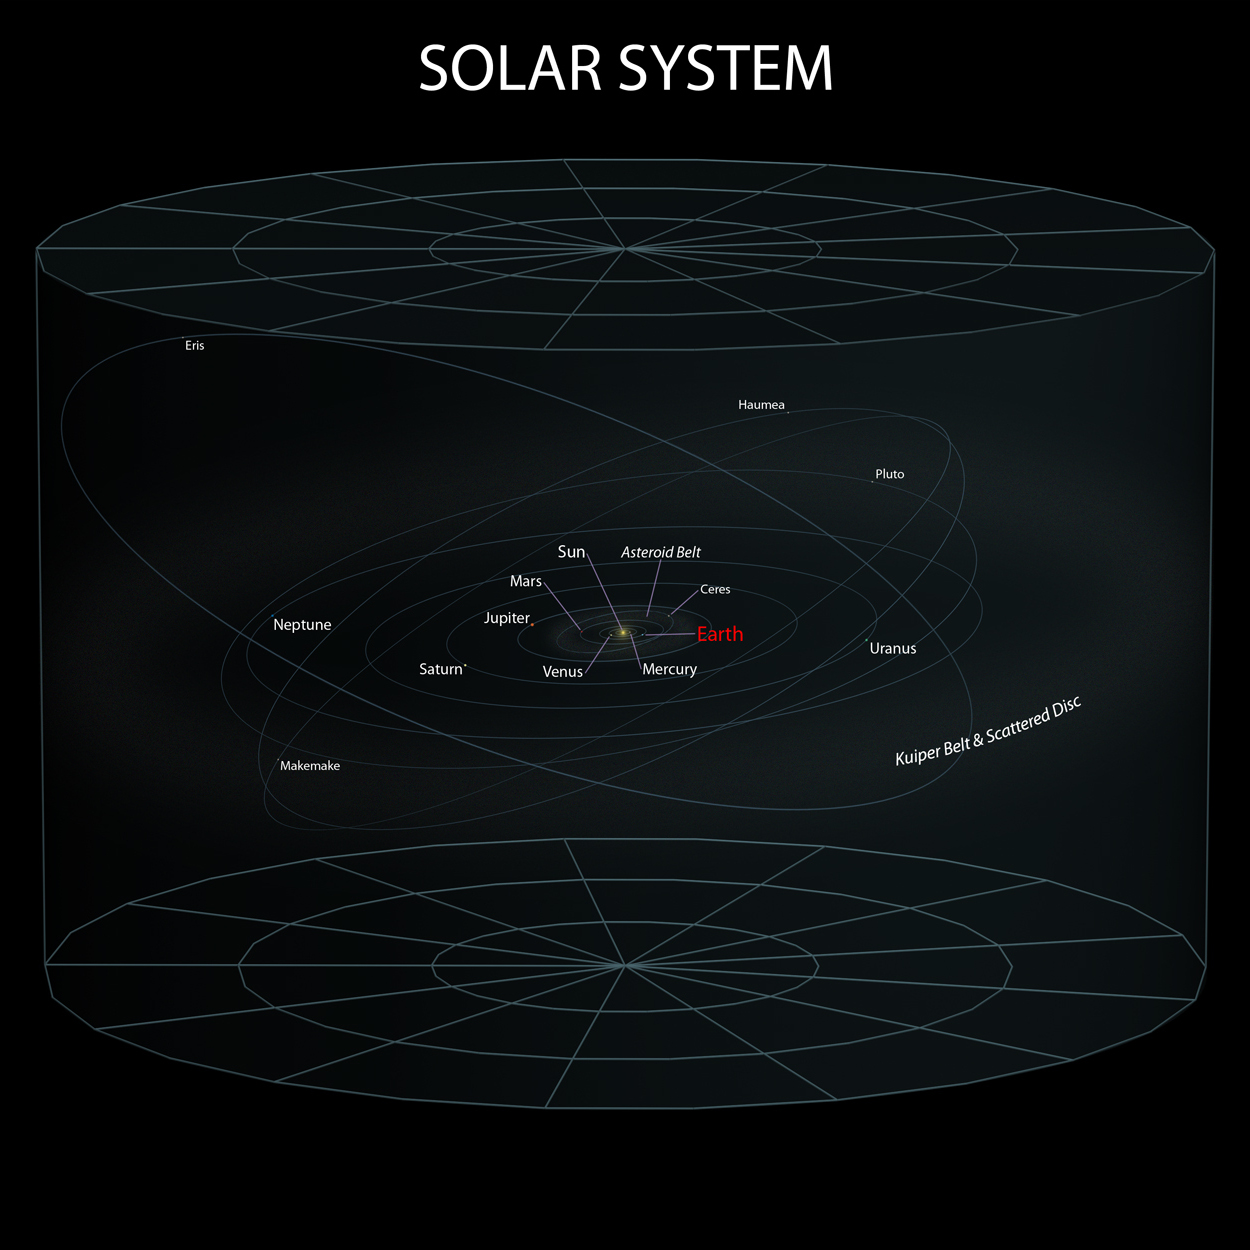
\includegraphics[width=\textwidth]{jwst/zoom_2.jpg}
                \column{0.49\textwidth}
                \begin{columns}
                    \column{0.49\textwidth}
                    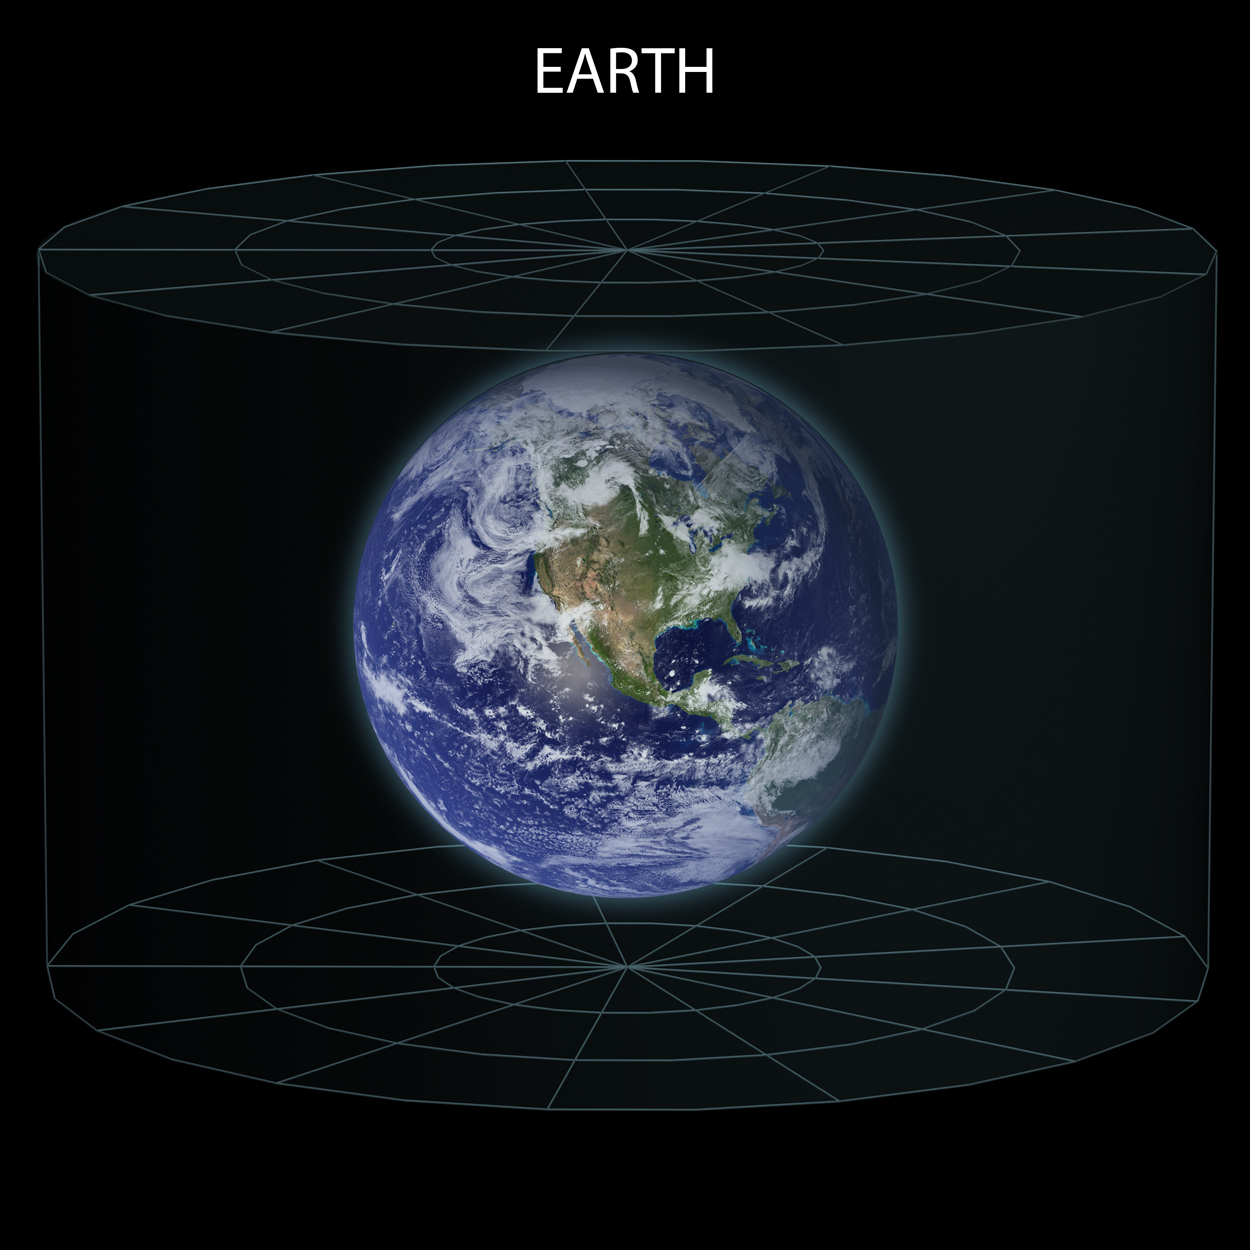
\includegraphics[width=\textwidth]{jwst/zoom_1.jpg}
                    \column{0.49\textwidth}
                \end{columns}
            \end{columns}
        \end{columns}
    \end{columns}
\end{frame}

\begin{frame}
    \frametitle{You are here}
    \begin{columns}
        \column{0.49\textwidth}
        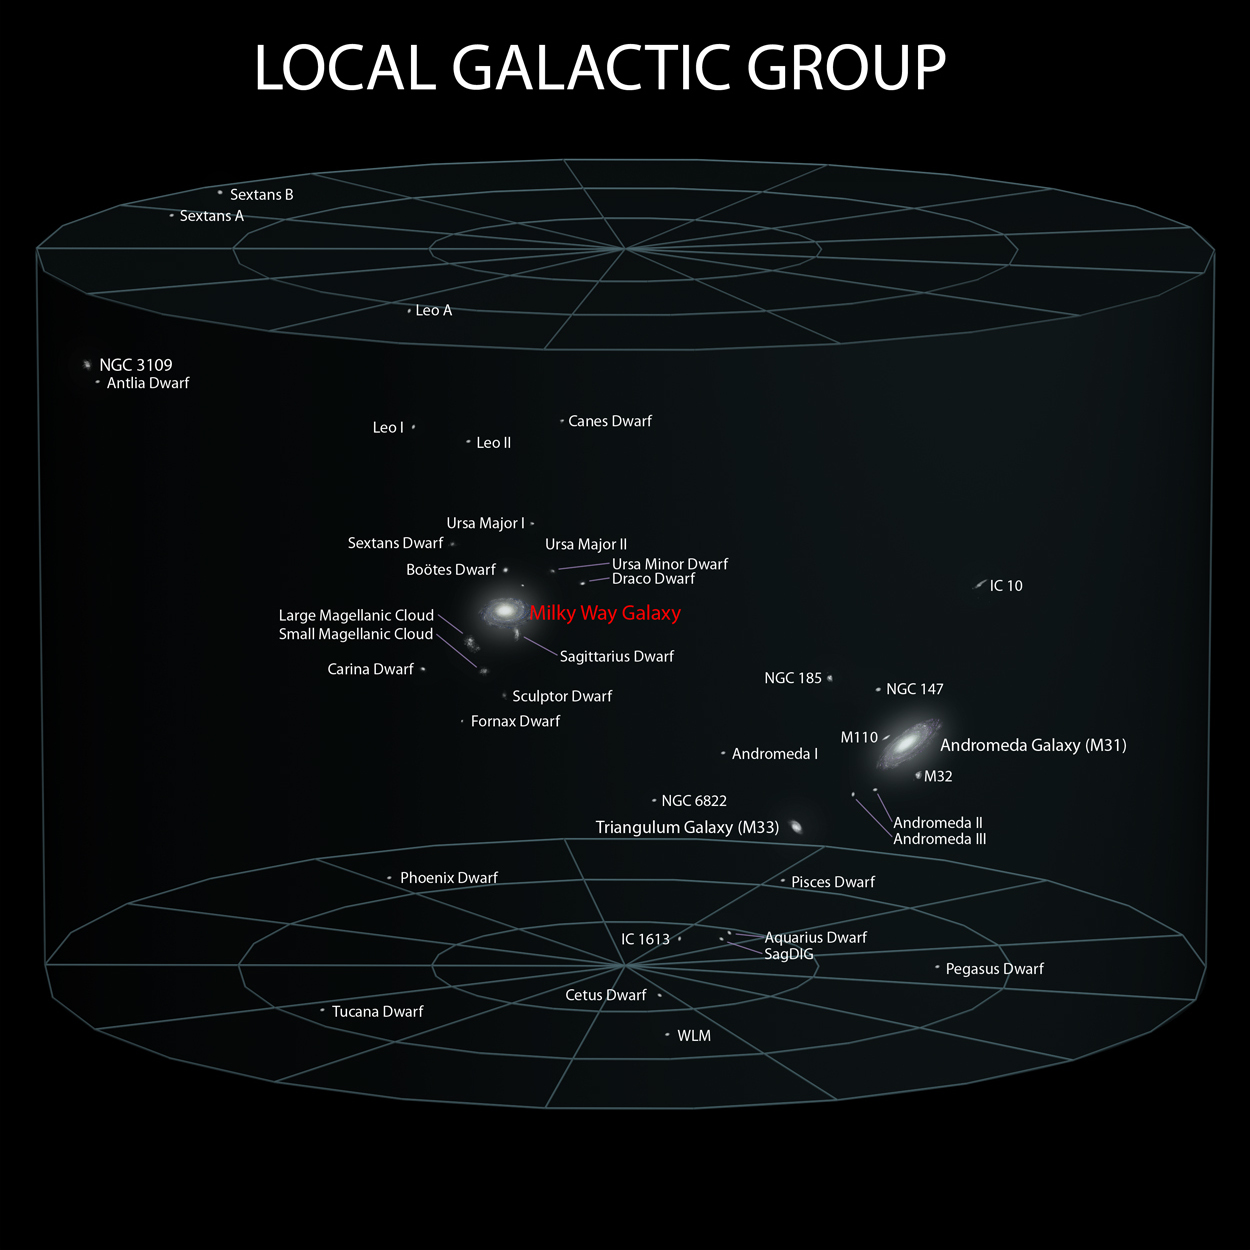
\includegraphics[width=\textwidth]{jwst/zoom_5.jpg}
        \column{0.49\textwidth}
        \begin{columns}
            \column{0.49\textwidth}
            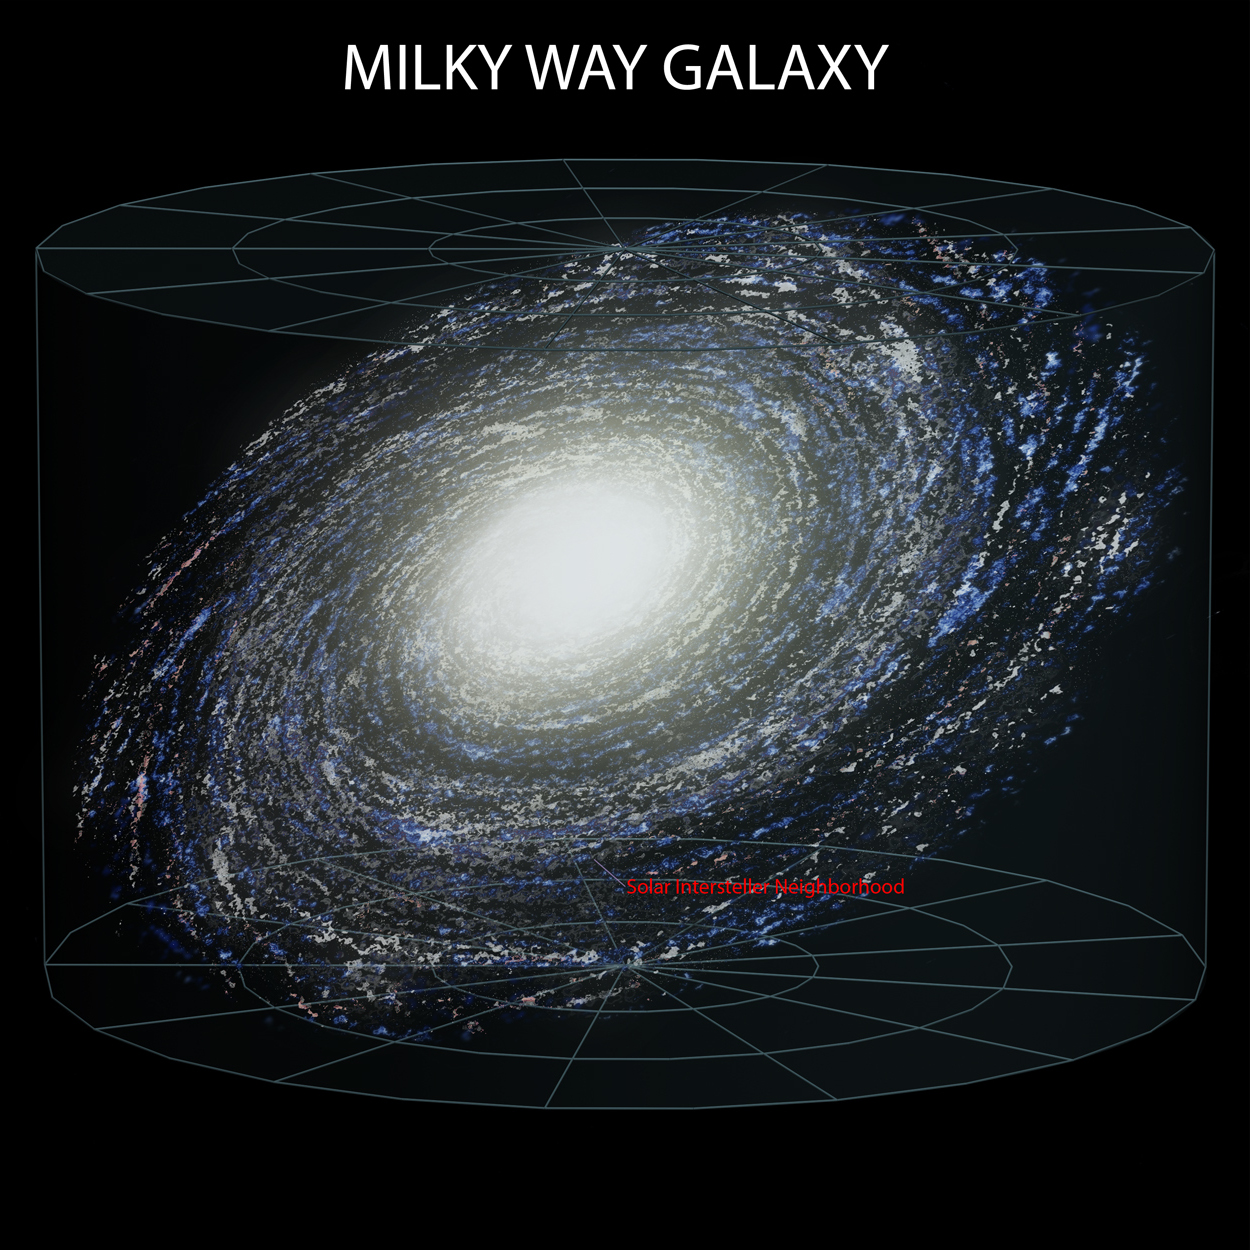
\includegraphics[width=\textwidth]{jwst/zoom_4.jpg}
            \column{0.49\textwidth}
            \begin{columns}
                \column{0.49\textwidth}
                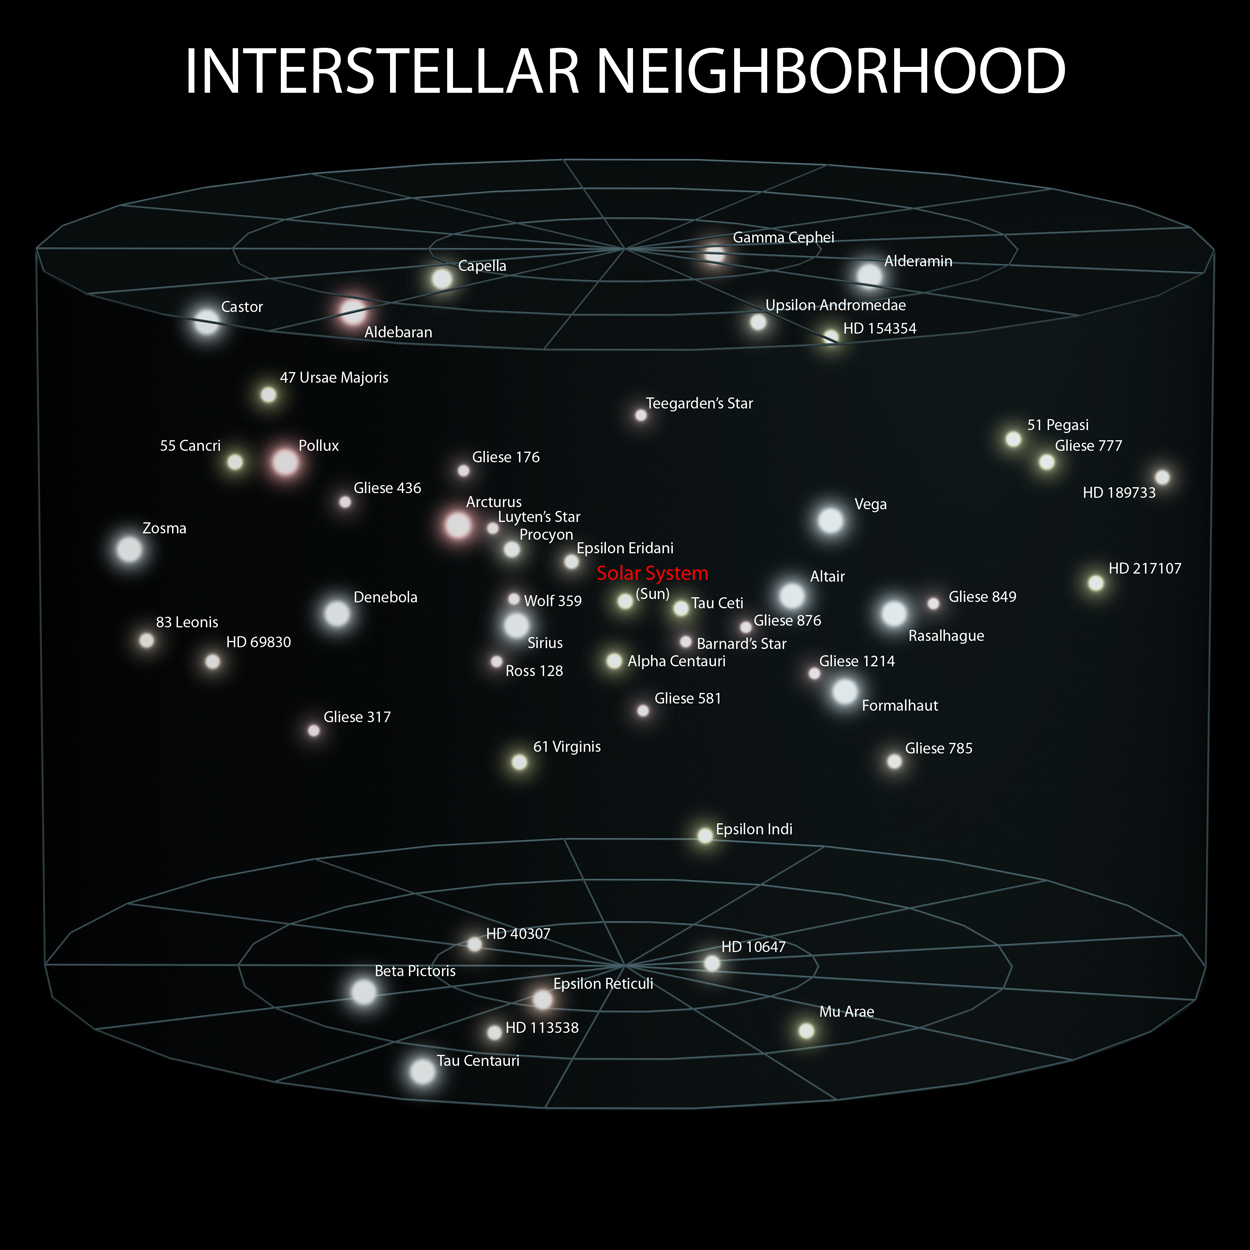
\includegraphics[width=\textwidth]{jwst/zoom_3.jpg}
                \column{0.49\textwidth}
                \begin{columns}
                    \column{0.49\textwidth}
                    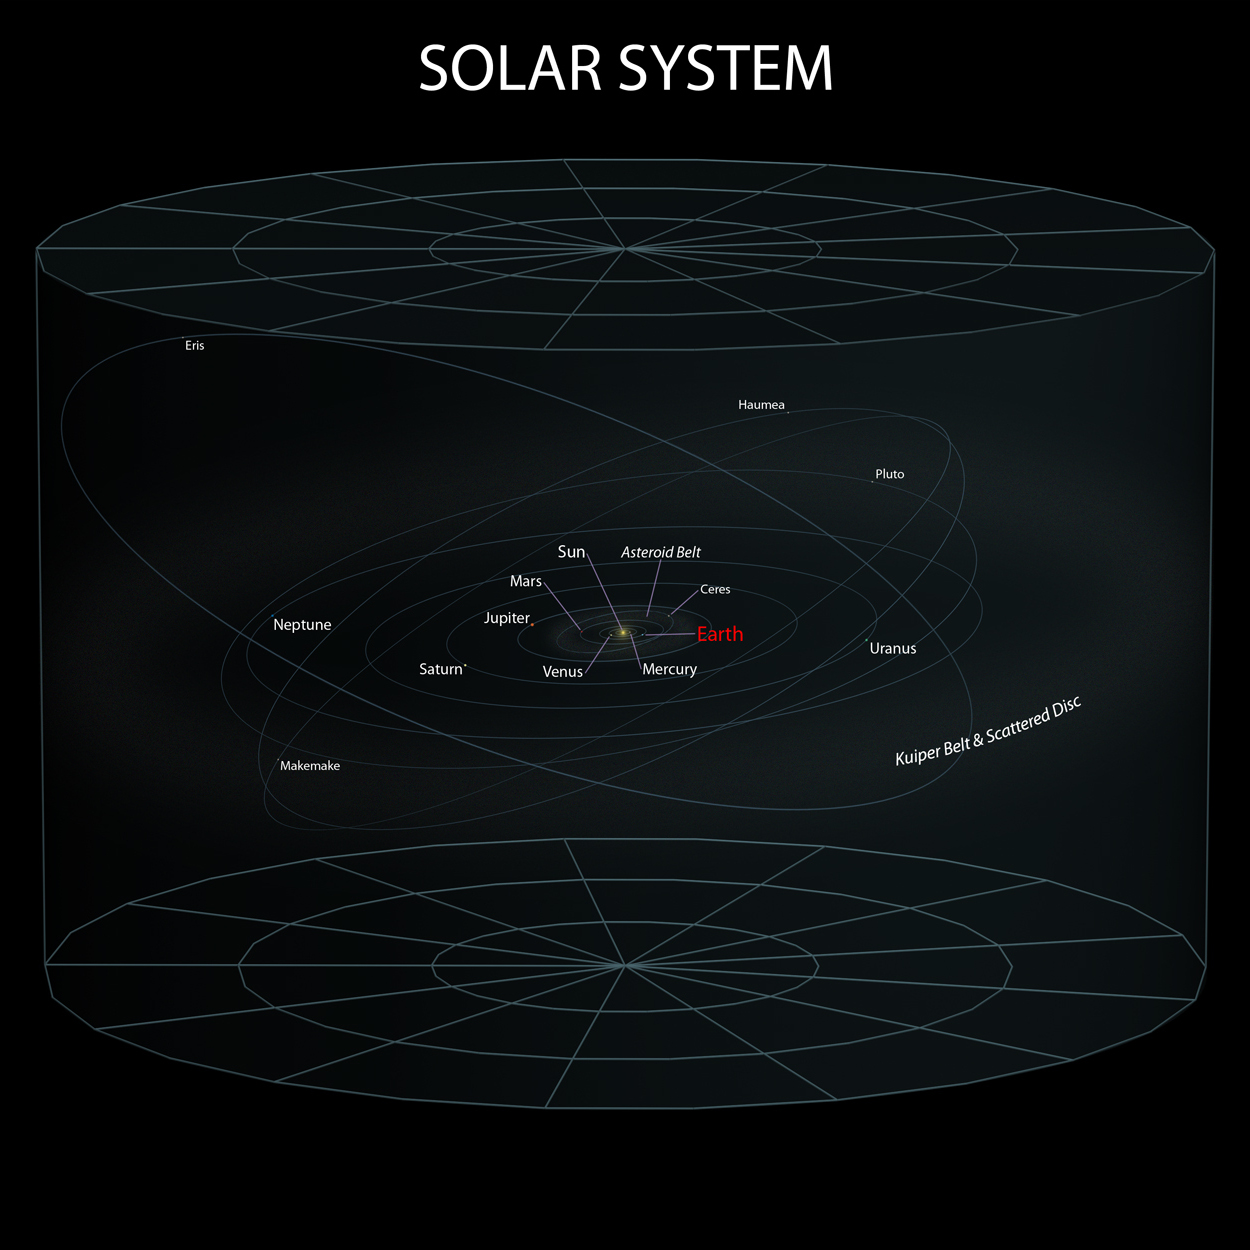
\includegraphics[width=\textwidth]{jwst/zoom_2.jpg}
                    \column{0.49\textwidth}
                    \begin{columns}
                        \column{0.49\textwidth}
                        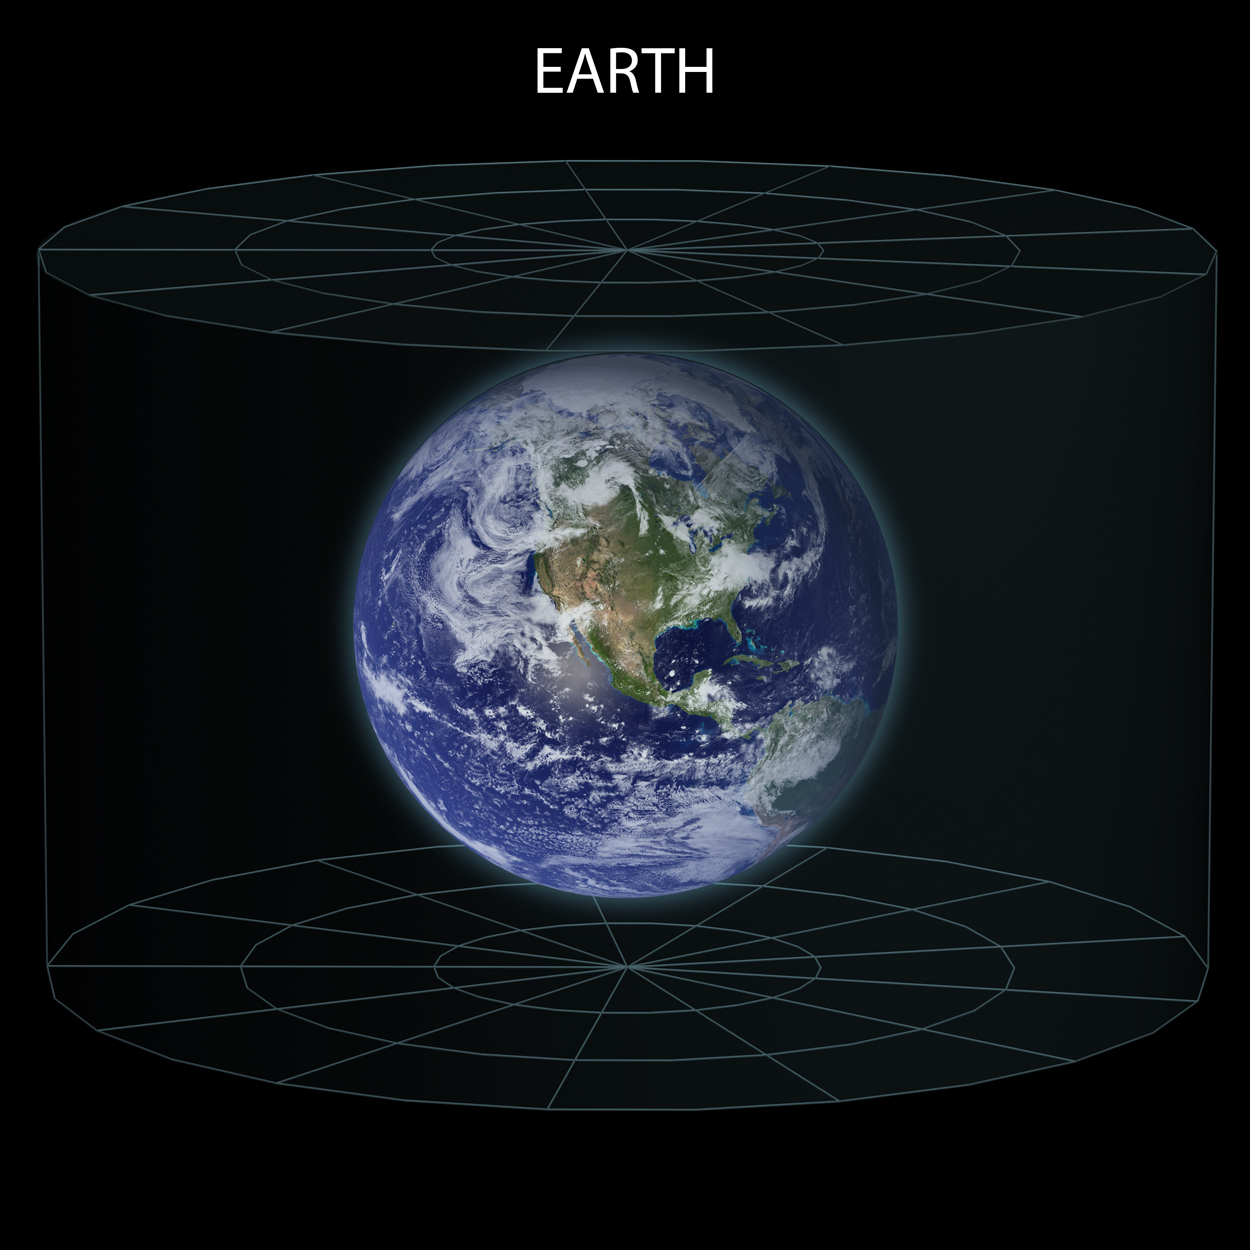
\includegraphics[width=\textwidth]{jwst/zoom_1.jpg}
                        \column{0.49\textwidth}
                    \end{columns}
                \end{columns}
            \end{columns}
        \end{columns}
    \end{columns}
\end{frame}

\begin{frame}
    \frametitle{You are here}
    \begin{columns}
        \column{0.49\textwidth}
        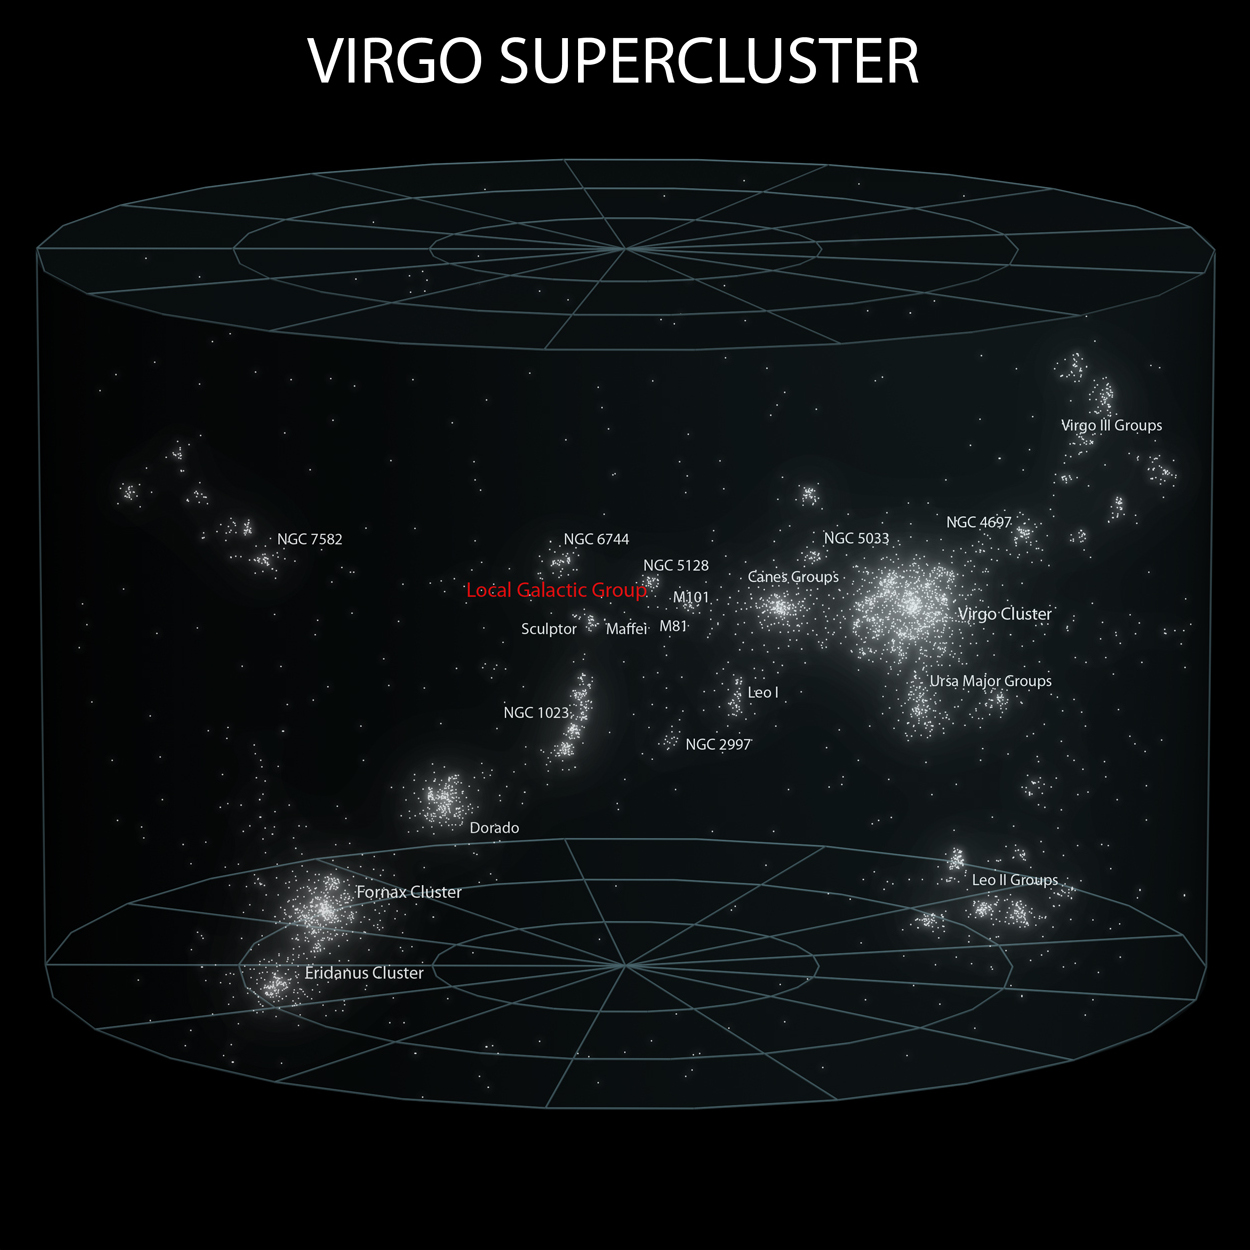
\includegraphics[width=\textwidth]{jwst/zoom_6.jpg}
        \column{0.49\textwidth}
        \begin{columns}
            \column{0.49\textwidth}
            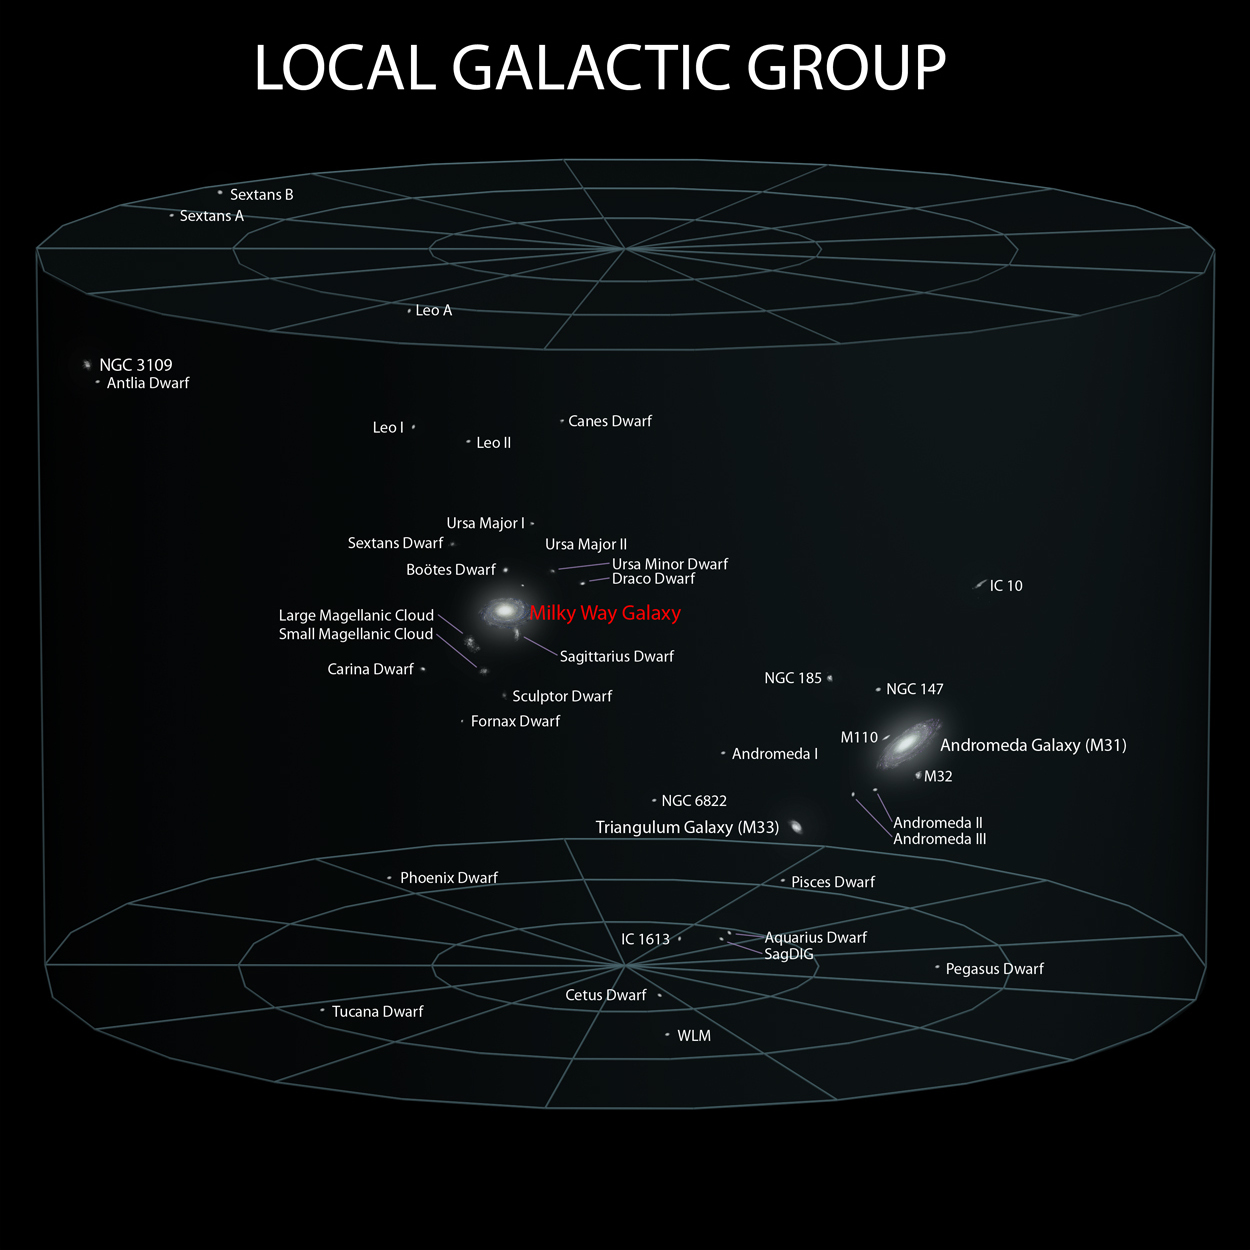
\includegraphics[width=\textwidth]{jwst/zoom_5.jpg}
            \column{0.49\textwidth}
            \begin{columns}
                \column{0.49\textwidth}
                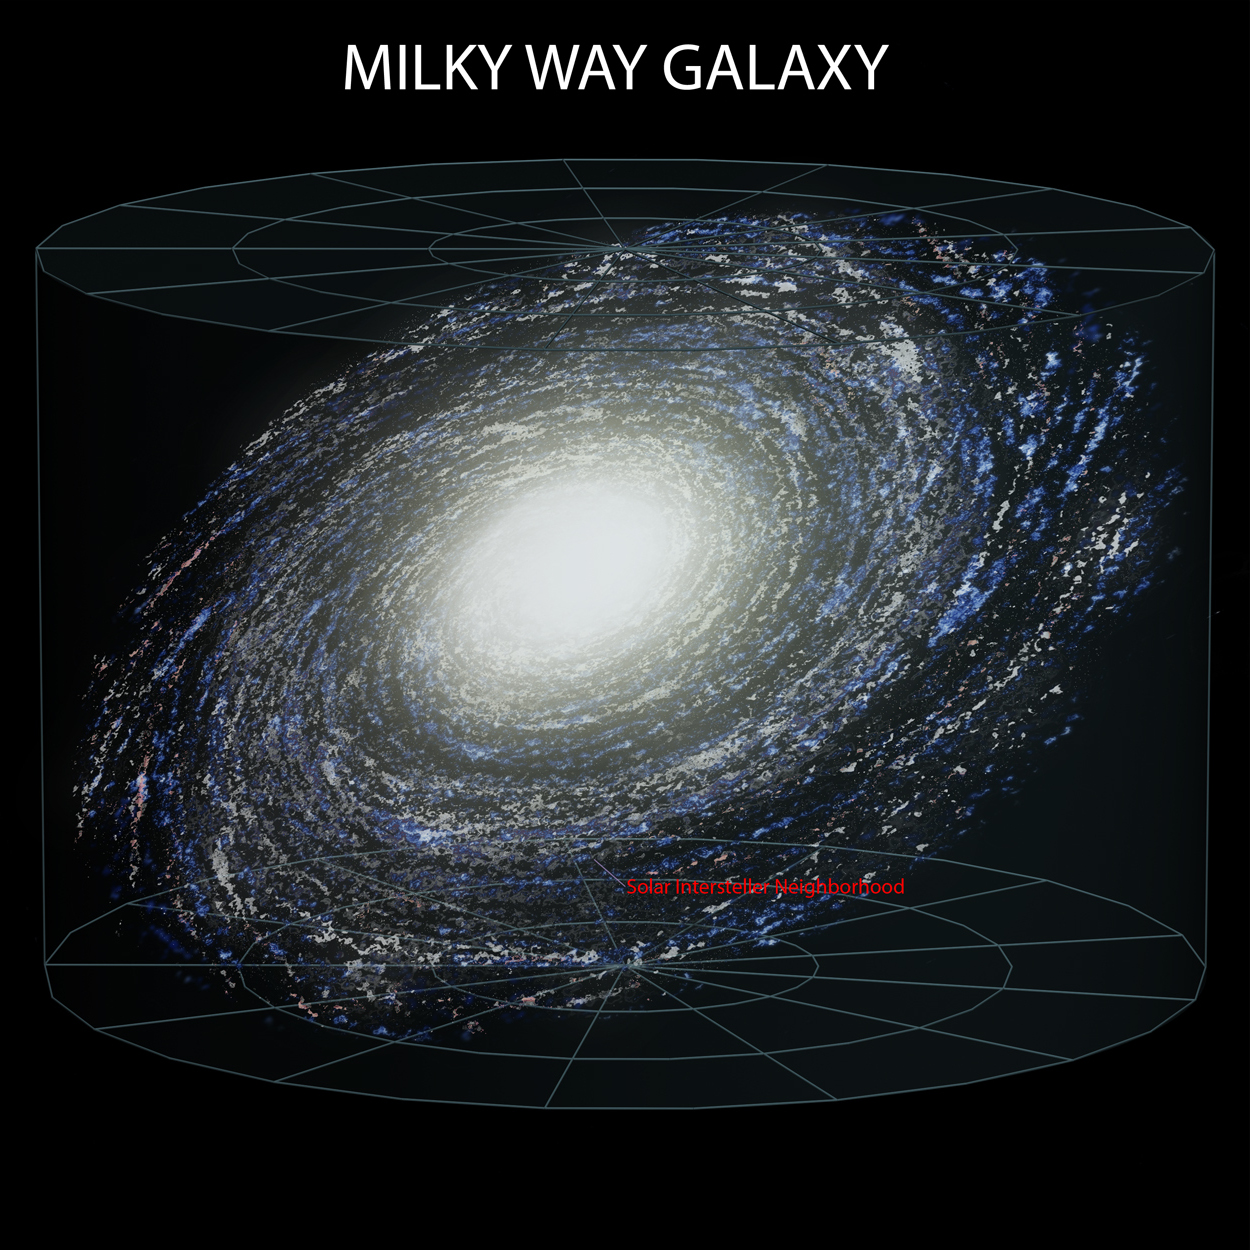
\includegraphics[width=\textwidth]{jwst/zoom_4.jpg}
                \column{0.49\textwidth}
                \begin{columns}
                    \column{0.49\textwidth}
                    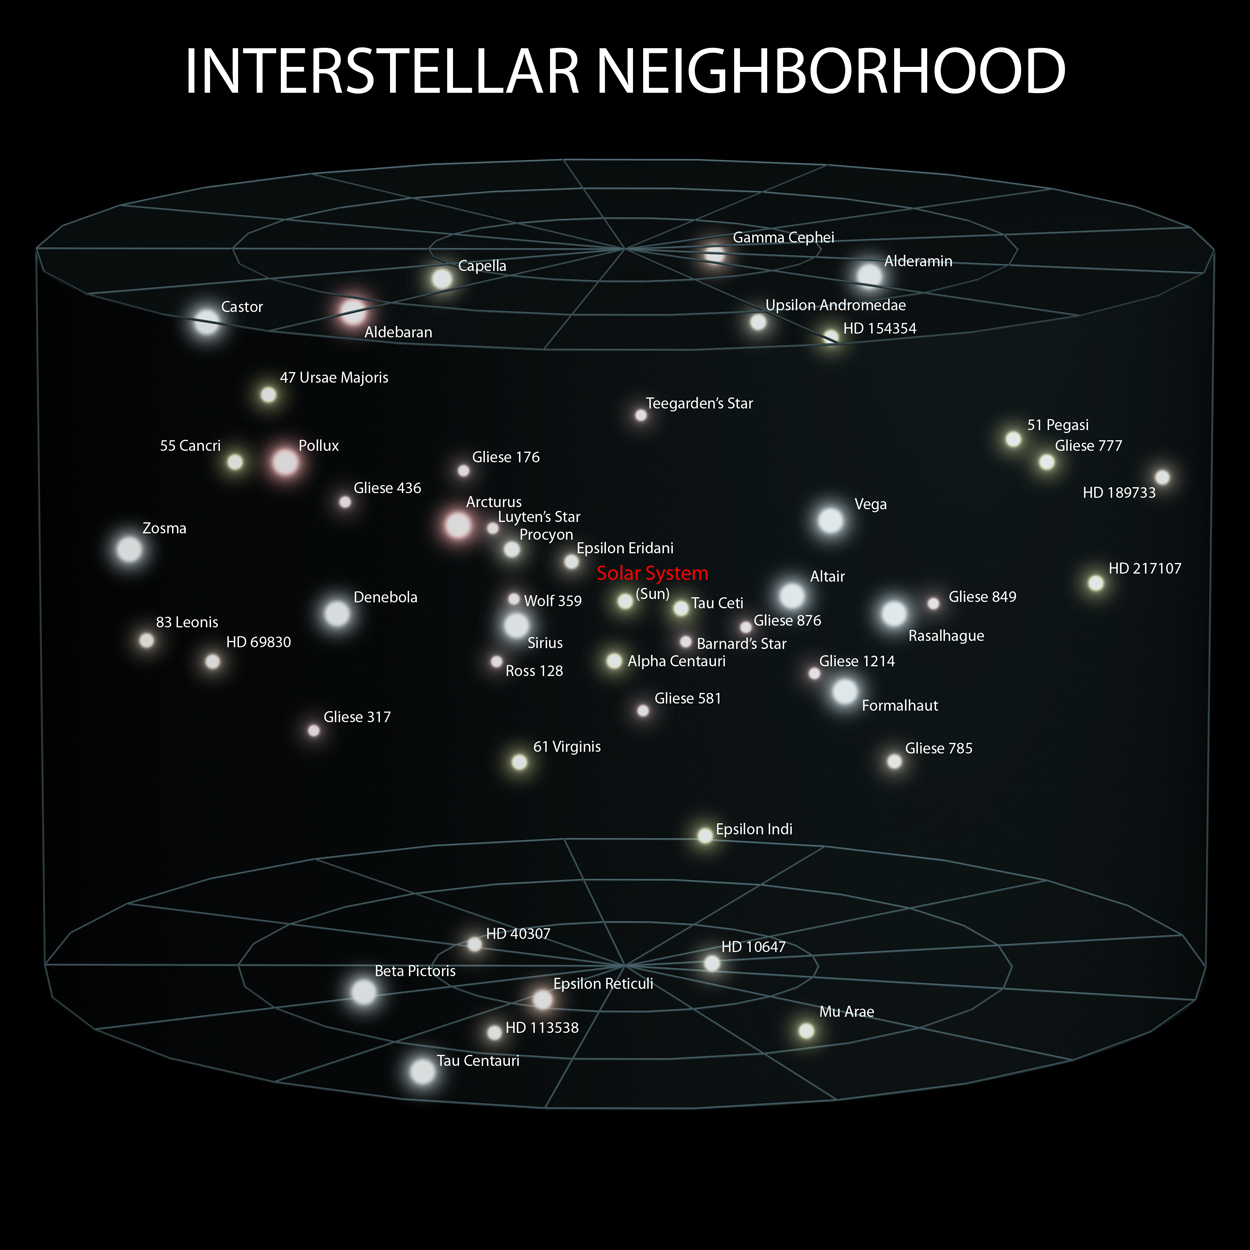
\includegraphics[width=\textwidth]{jwst/zoom_3.jpg}
                    \column{0.49\textwidth}
                    \begin{columns}
                        \column{0.49\textwidth}
                        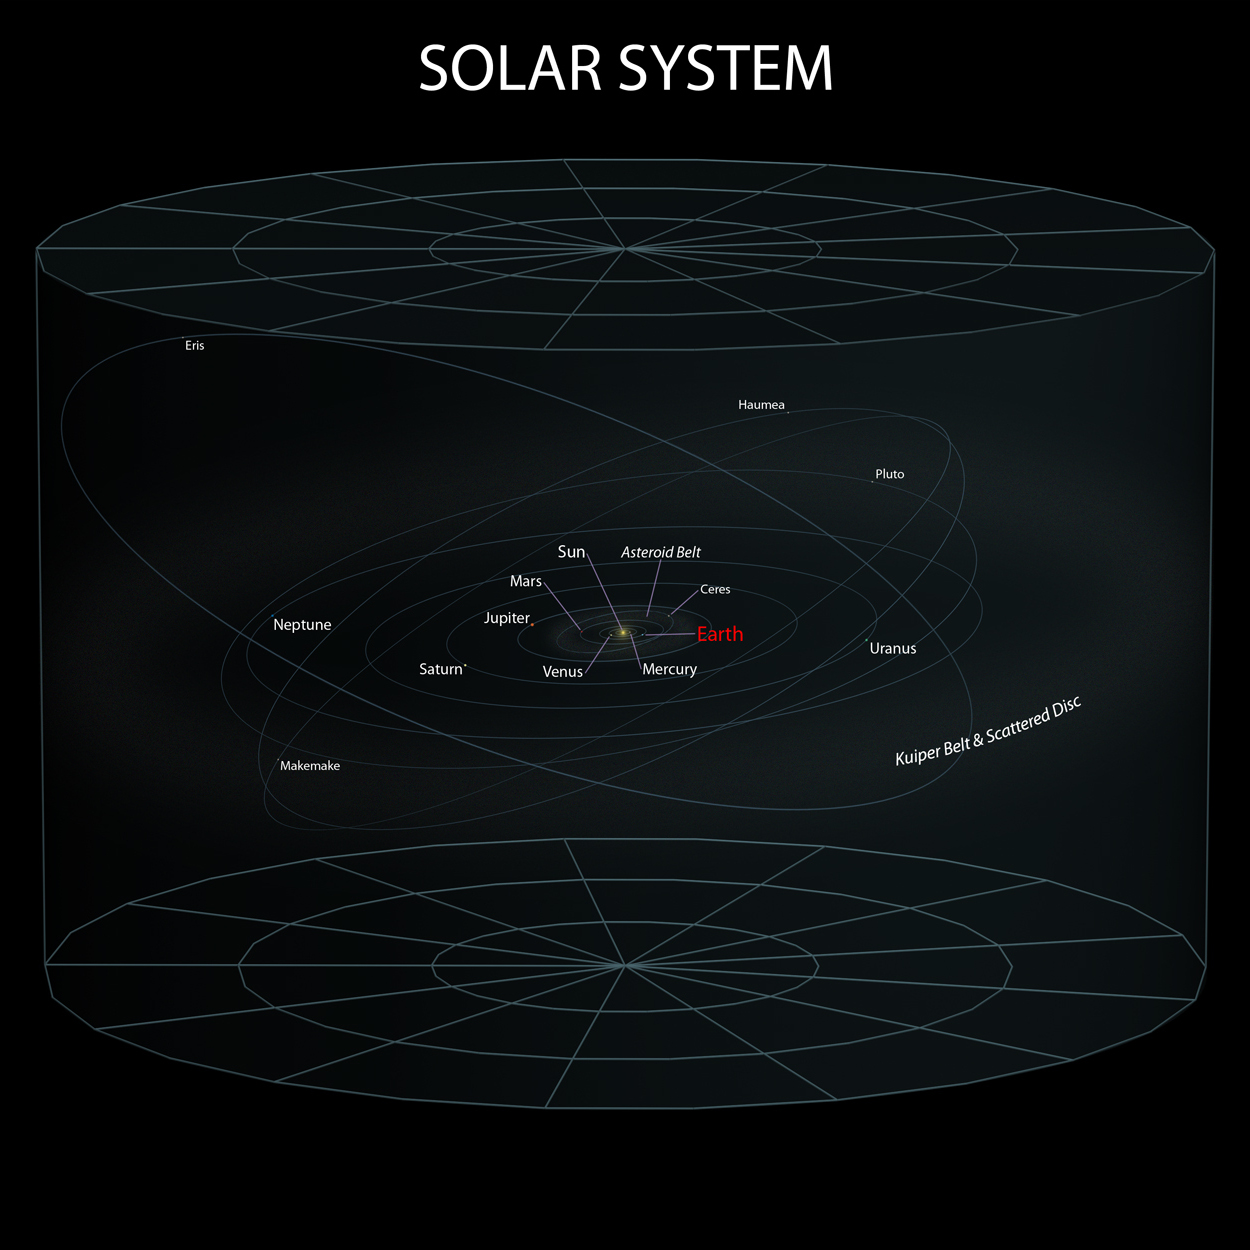
\includegraphics[width=\textwidth]{jwst/zoom_2.jpg}
                        \column{0.49\textwidth}
                        \begin{columns}
                            \column{0.49\textwidth}
                            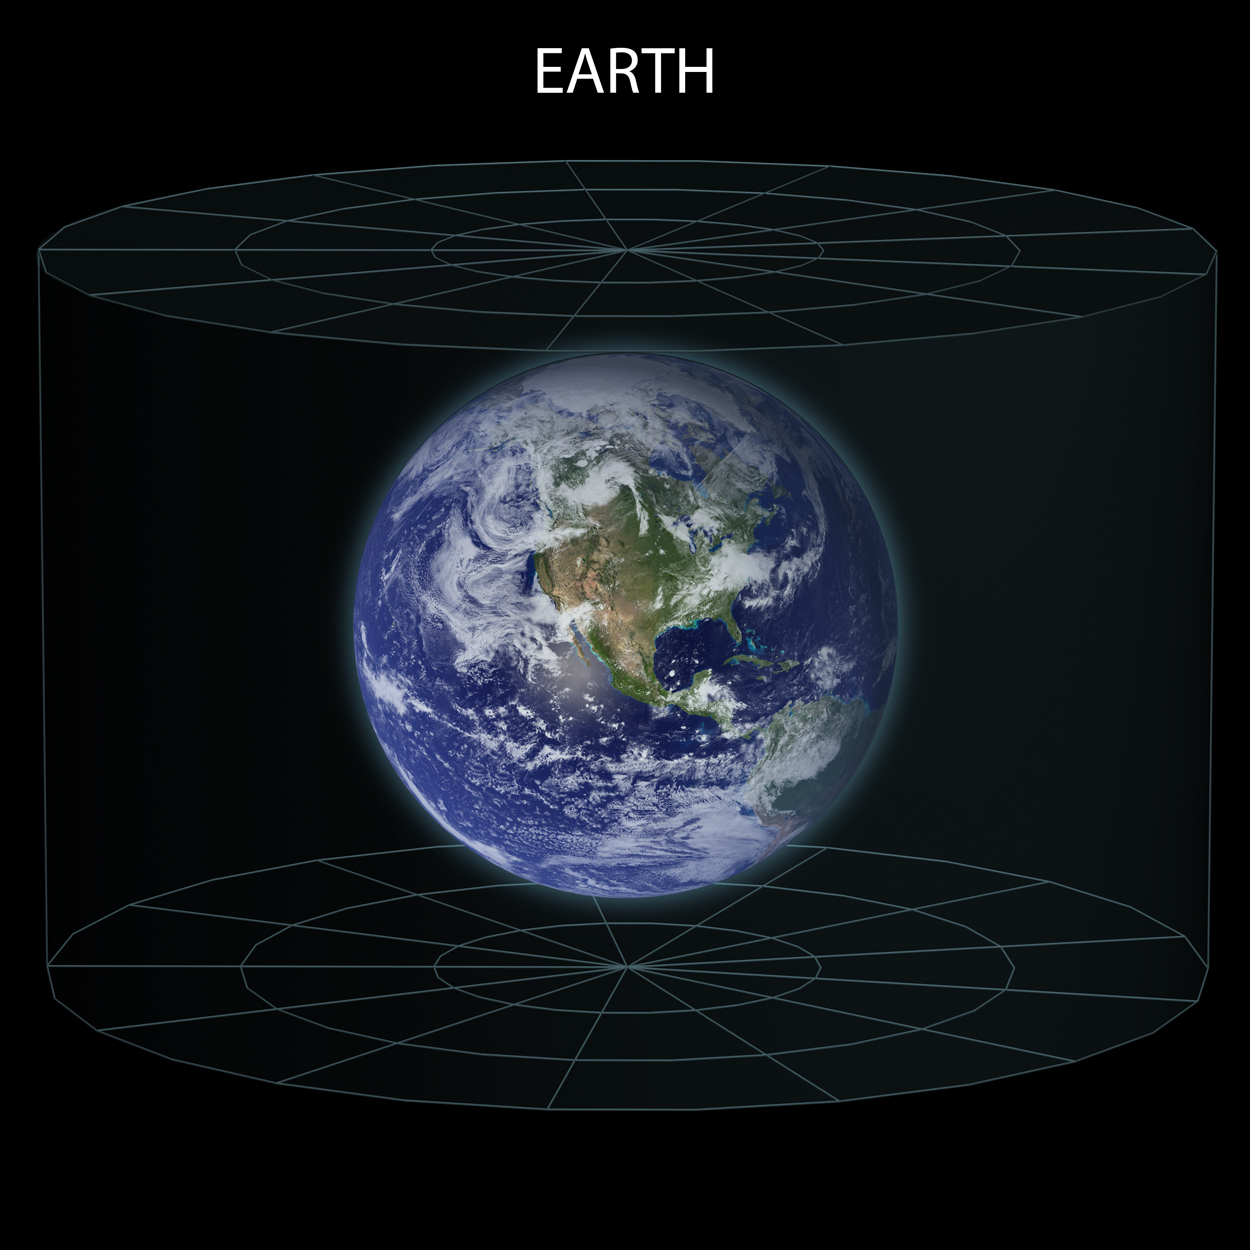
\includegraphics[width=\textwidth]{jwst/zoom_1.jpg}
                            \column{0.49\textwidth}
                        \end{columns}
                    \end{columns}
                \end{columns}
            \end{columns}
        \end{columns}
    \end{columns}
\end{frame}

\begin{frame}
    \frametitle{You are here}
    \begin{columns}
        \column{0.49\textwidth}
        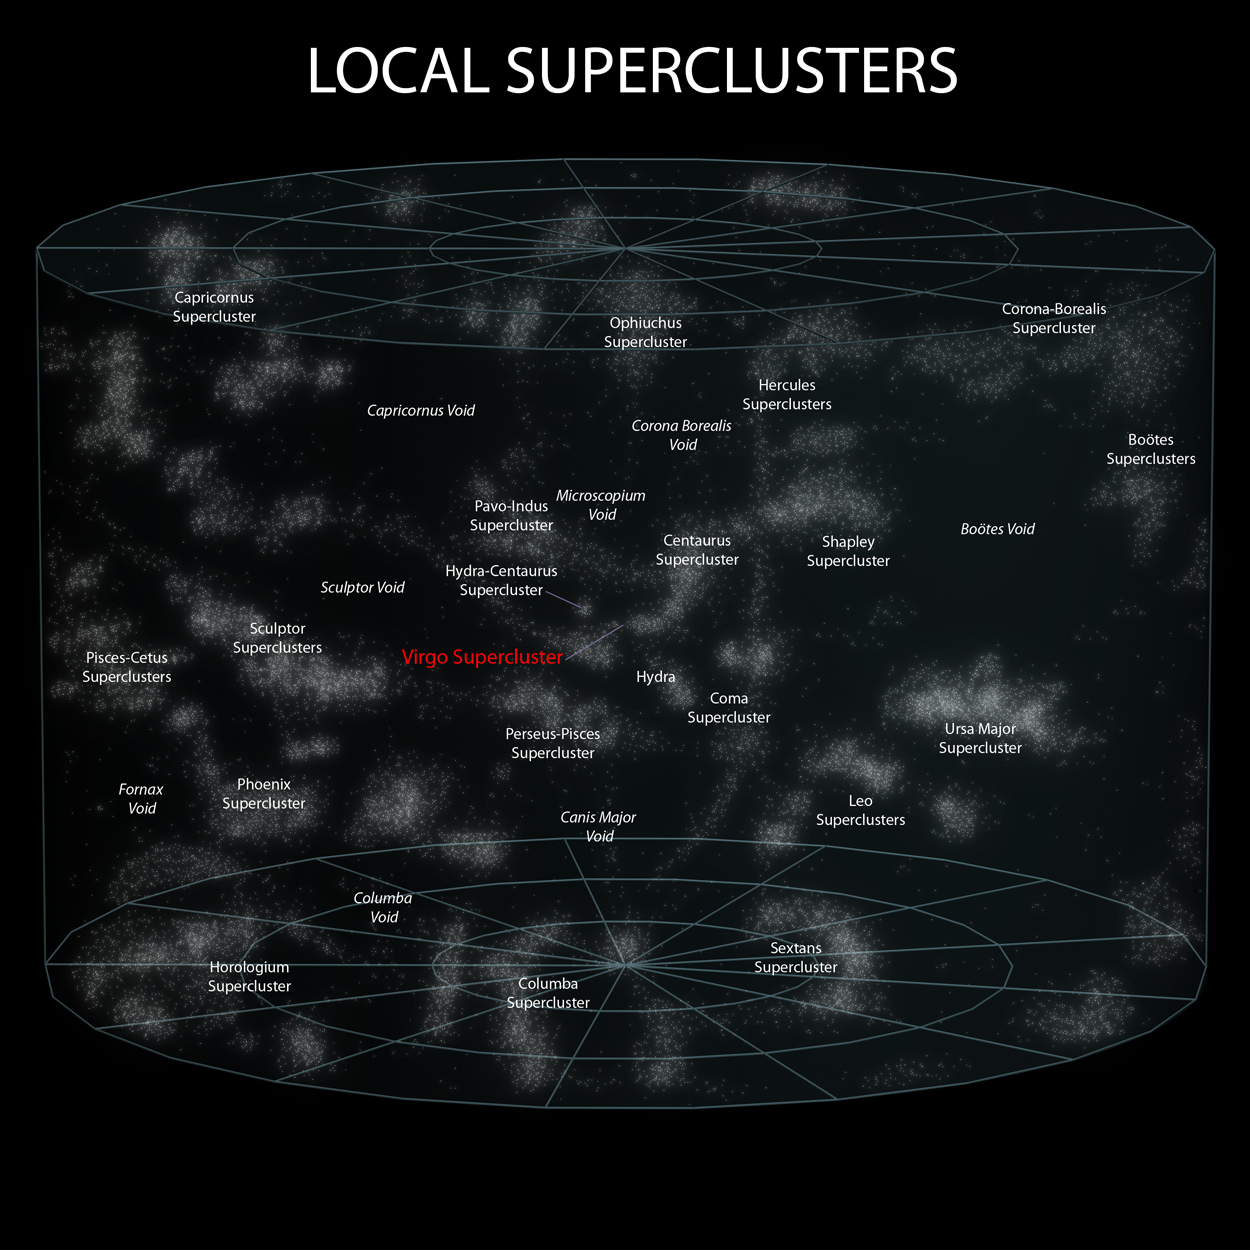
\includegraphics[width=\textwidth]{jwst/zoom_7.jpg}
        \column{0.49\textwidth}
        \begin{columns}
            \column{0.49\textwidth}
            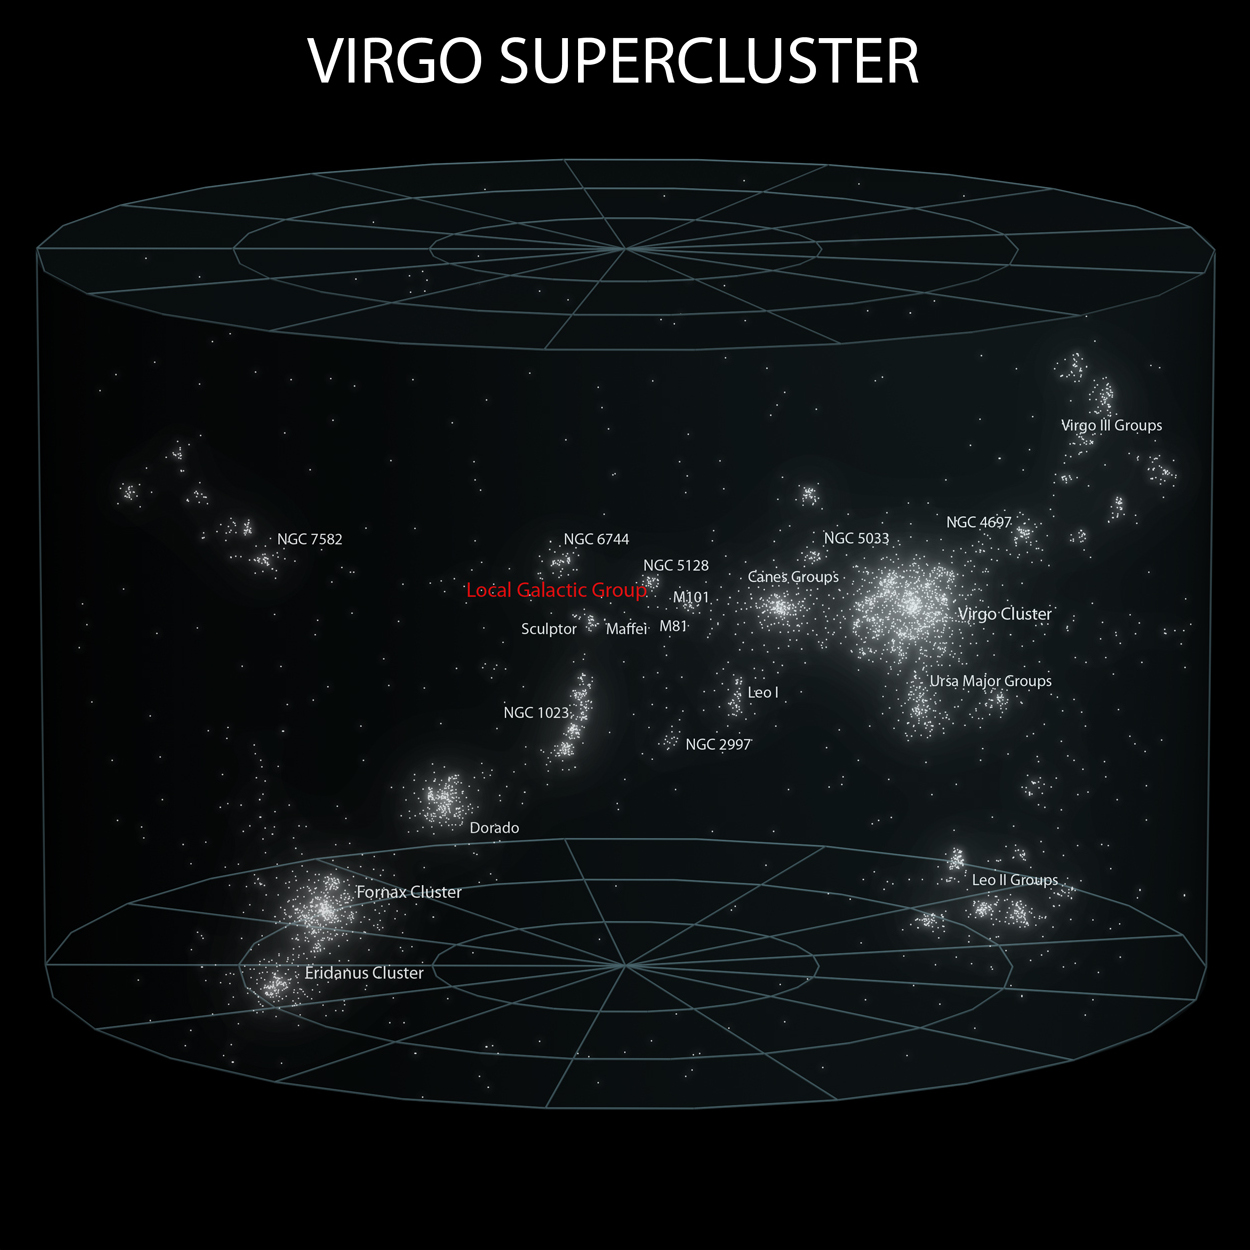
\includegraphics[width=\textwidth]{jwst/zoom_6.jpg}
            \column{0.49\textwidth}
            \begin{columns}
                \column{0.49\textwidth}
                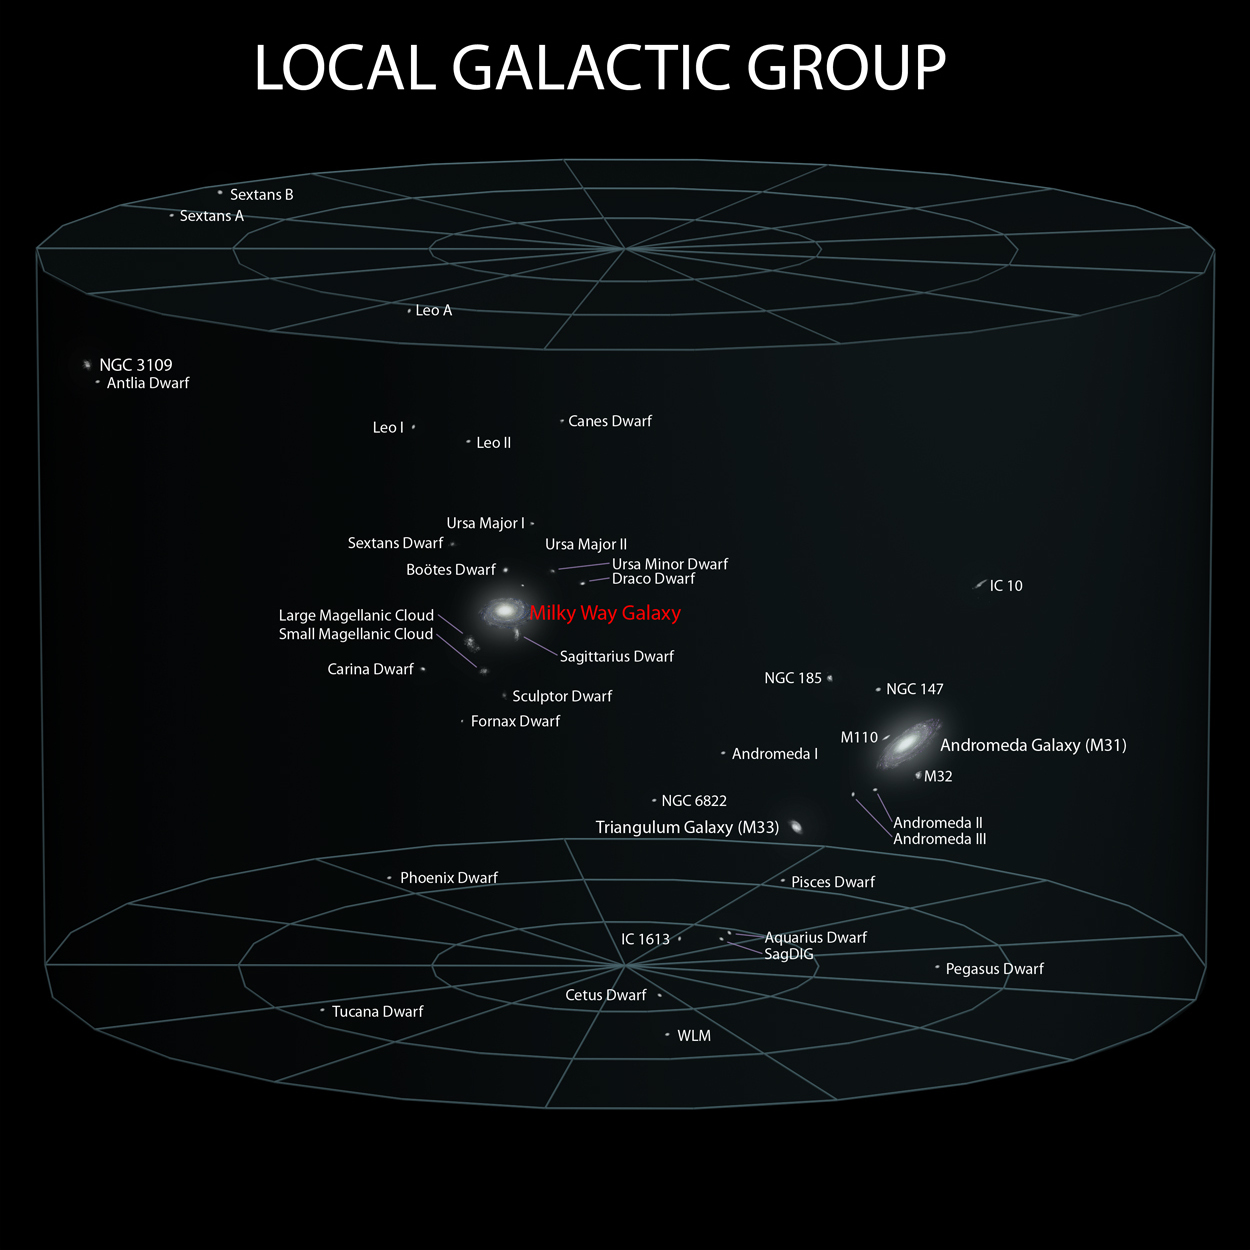
\includegraphics[width=\textwidth]{jwst/zoom_5.jpg}
                \column{0.49\textwidth}
                \begin{columns}
                    \column{0.49\textwidth}
                    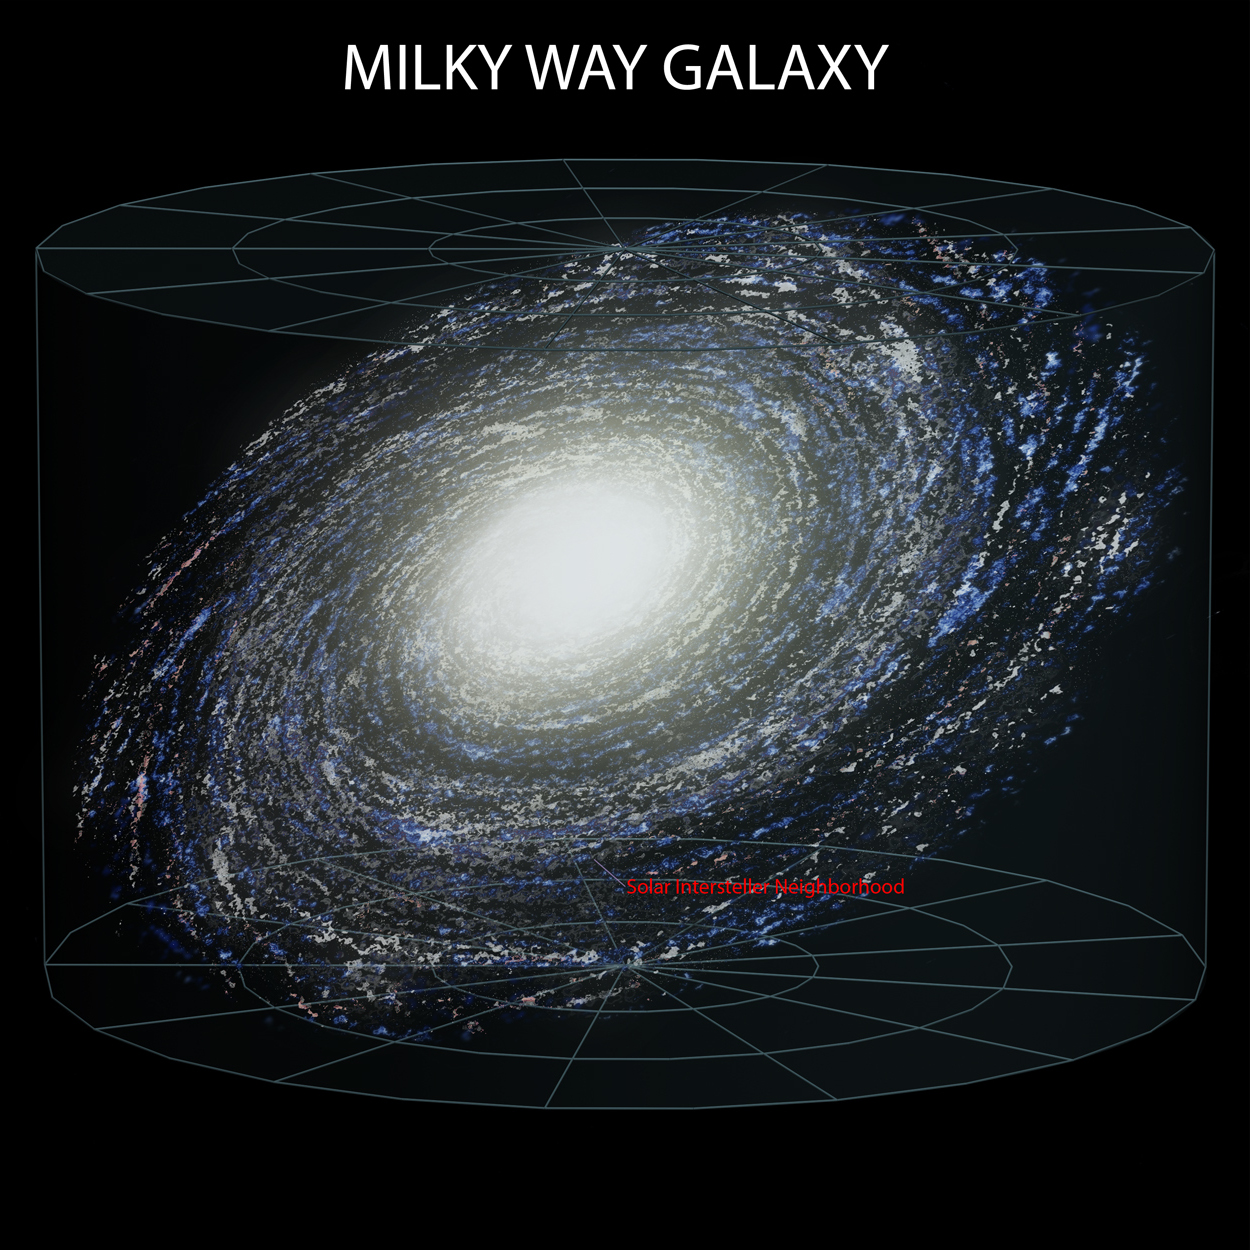
\includegraphics[width=\textwidth]{jwst/zoom_4.jpg}
                    \column{0.49\textwidth}
                    \begin{columns}
                        \column{0.49\textwidth}
                        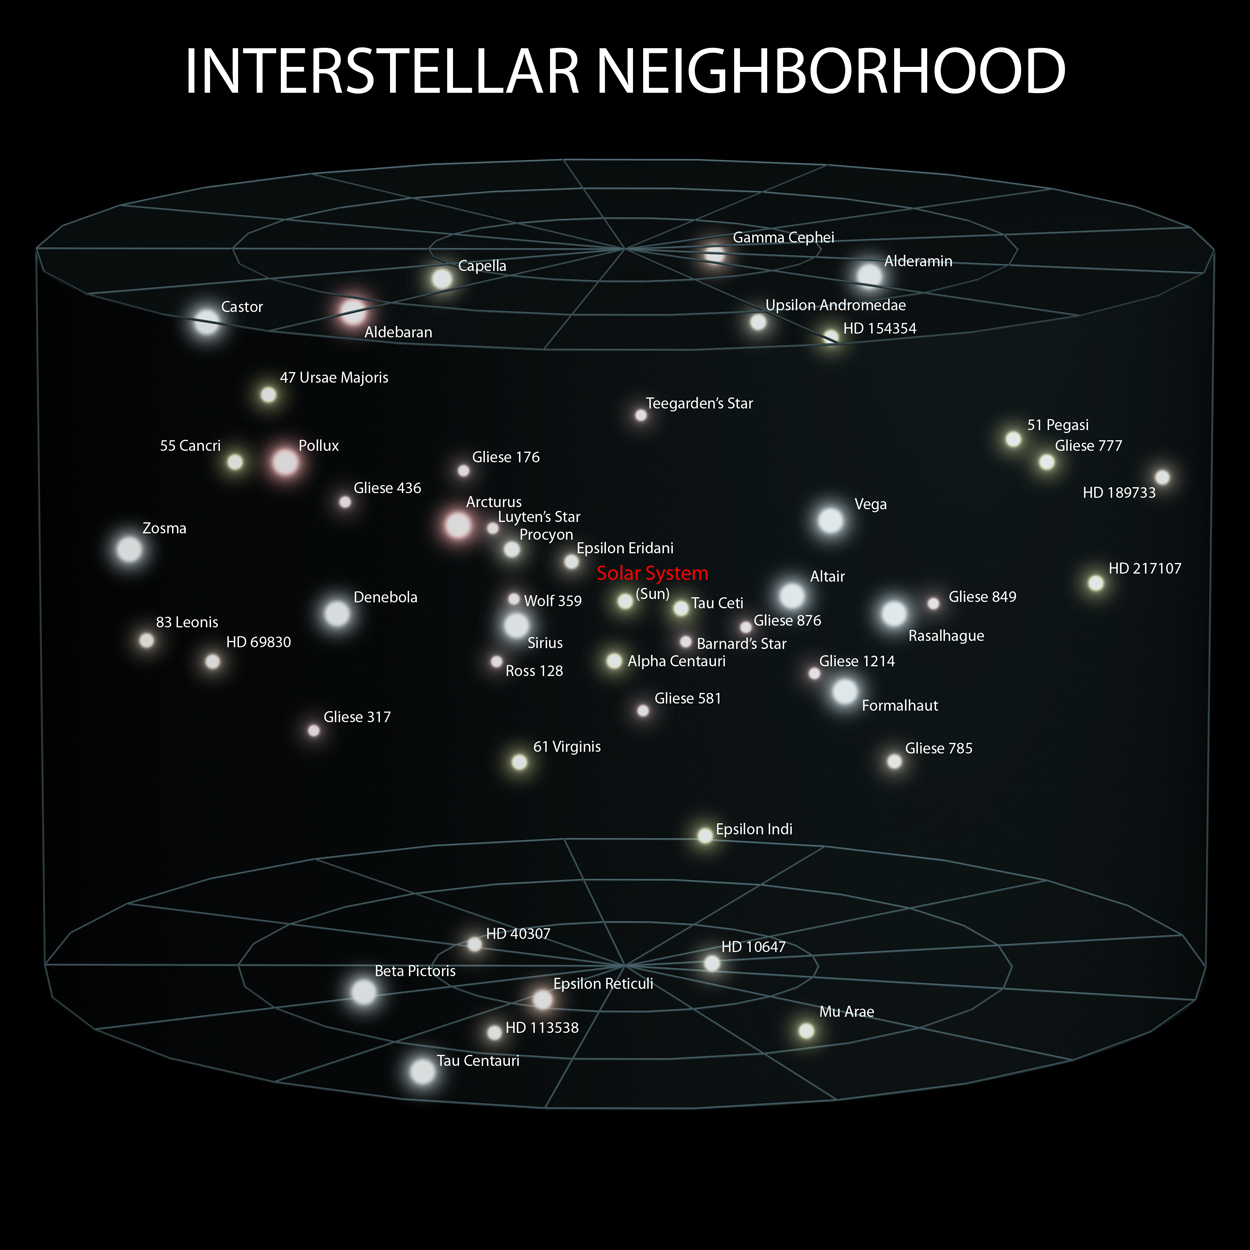
\includegraphics[width=\textwidth]{jwst/zoom_3.jpg}
                        \column{0.49\textwidth}
                        \begin{columns}
                            \column{0.49\textwidth}
                            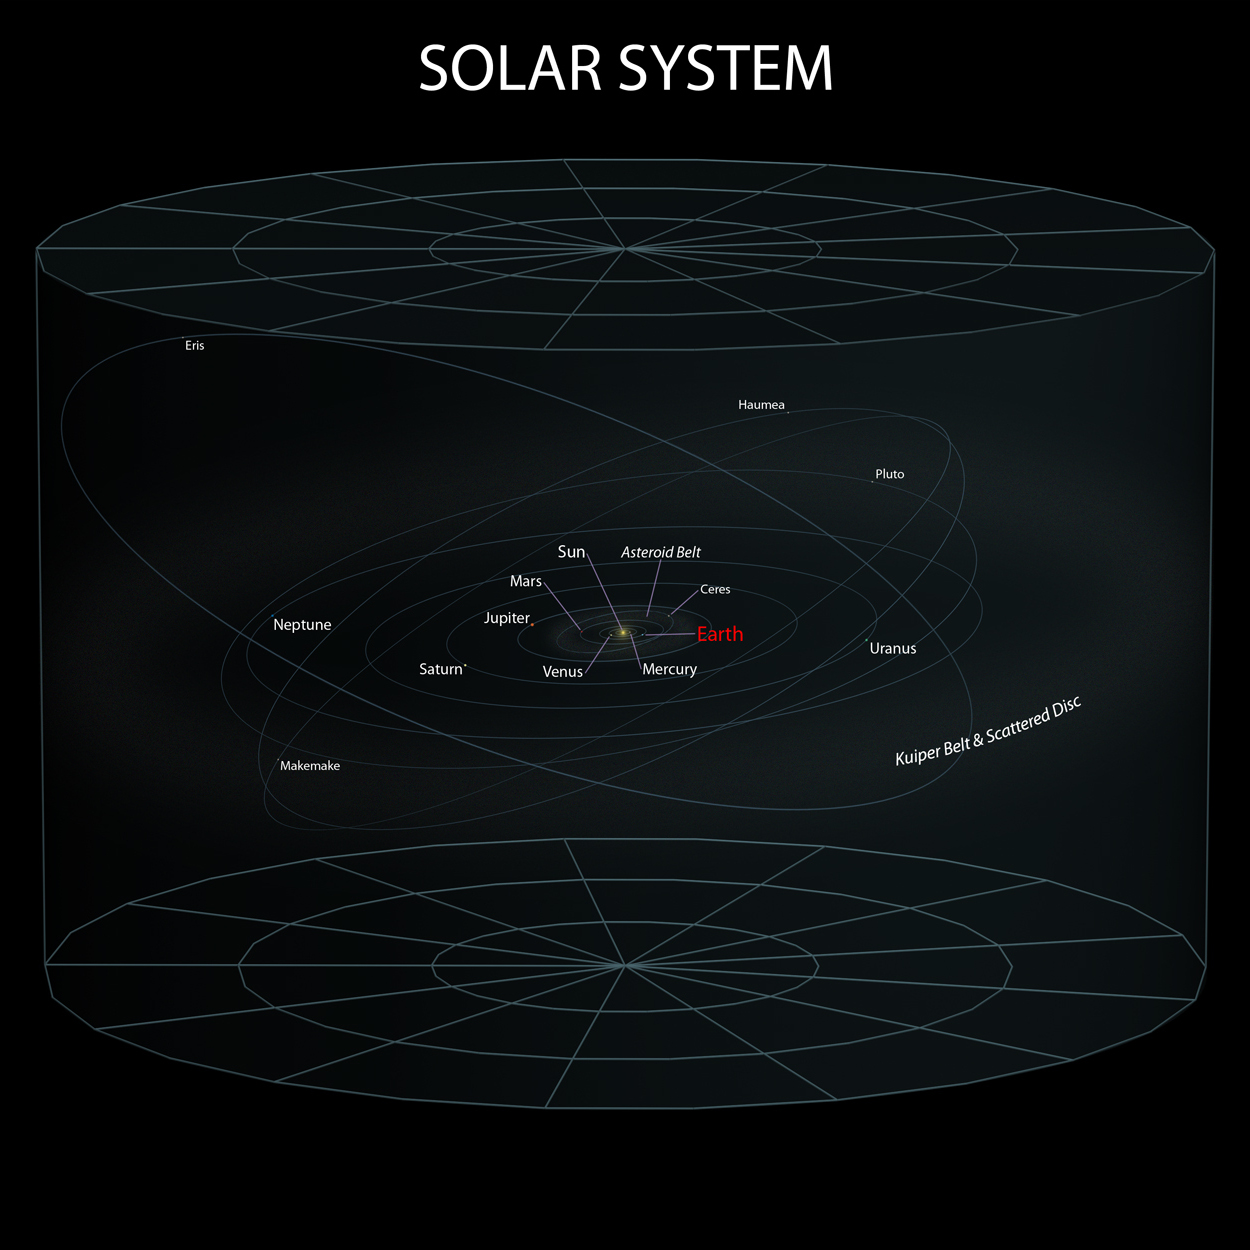
\includegraphics[width=\textwidth]{jwst/zoom_2.jpg}
                            \column{0.49\textwidth}
                            \begin{columns}
                                \column{0.49\textwidth}
                                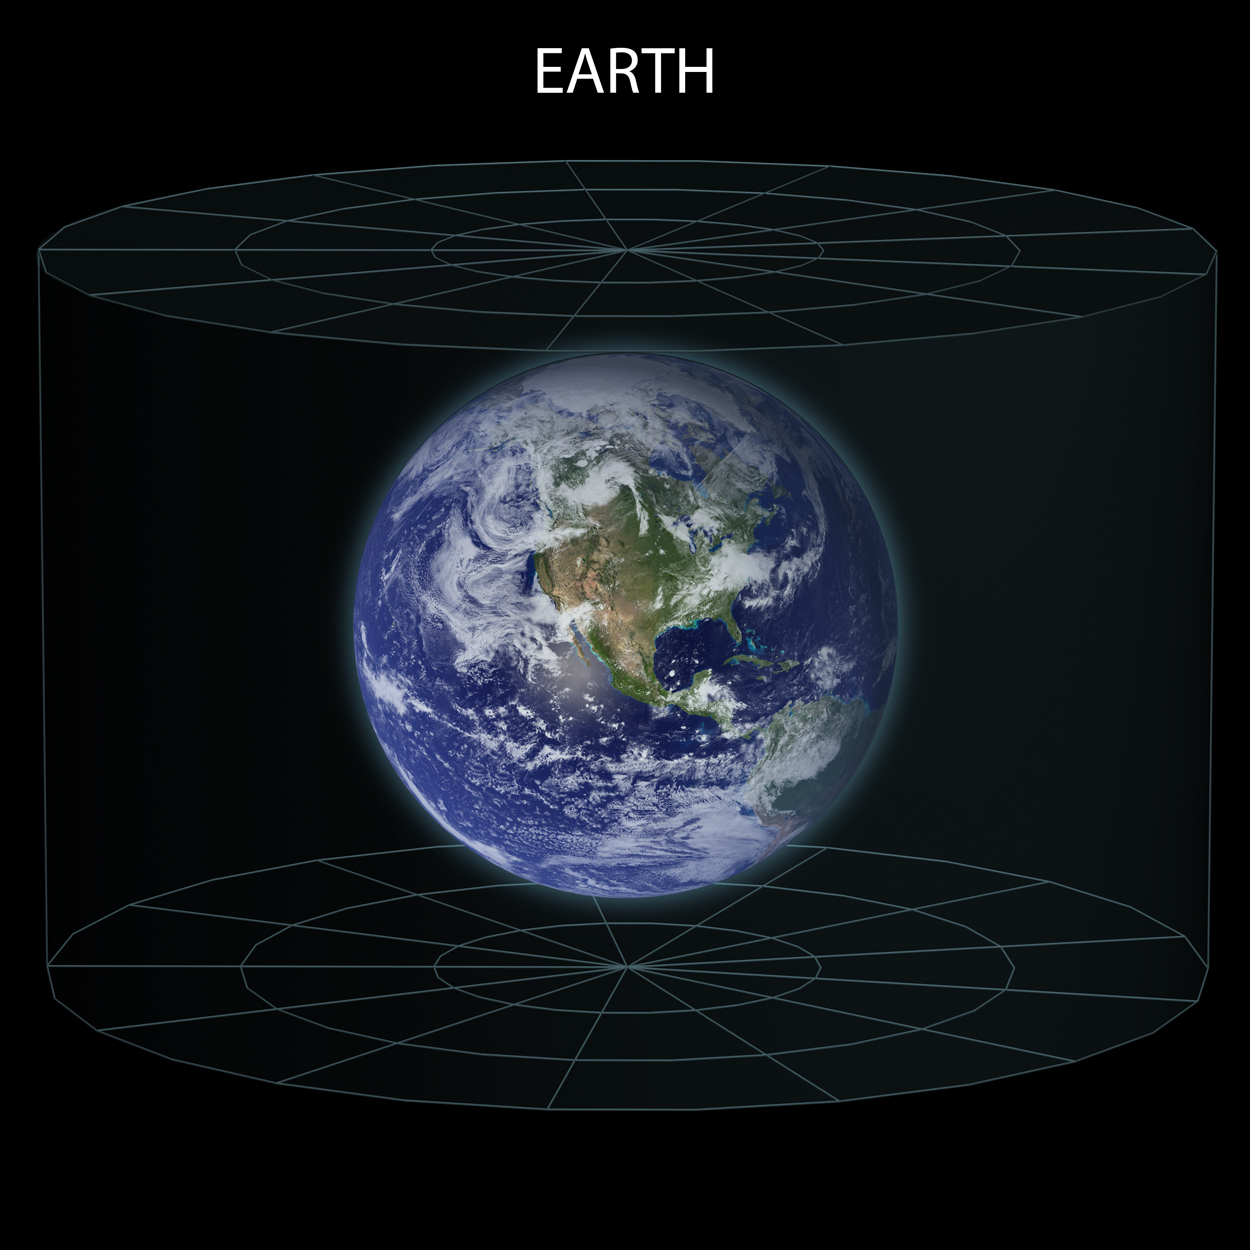
\includegraphics[width=\textwidth]{jwst/zoom_1.jpg}
                                \column{0.49\textwidth}
                            \end{columns}
                        \end{columns}
                    \end{columns}
                \end{columns}
            \end{columns}
        \end{columns}
    \end{columns}
\end{frame}

\begin{frame}
    \frametitle{You are here}
    \begin{columns}
        \column{0.49\textwidth}
        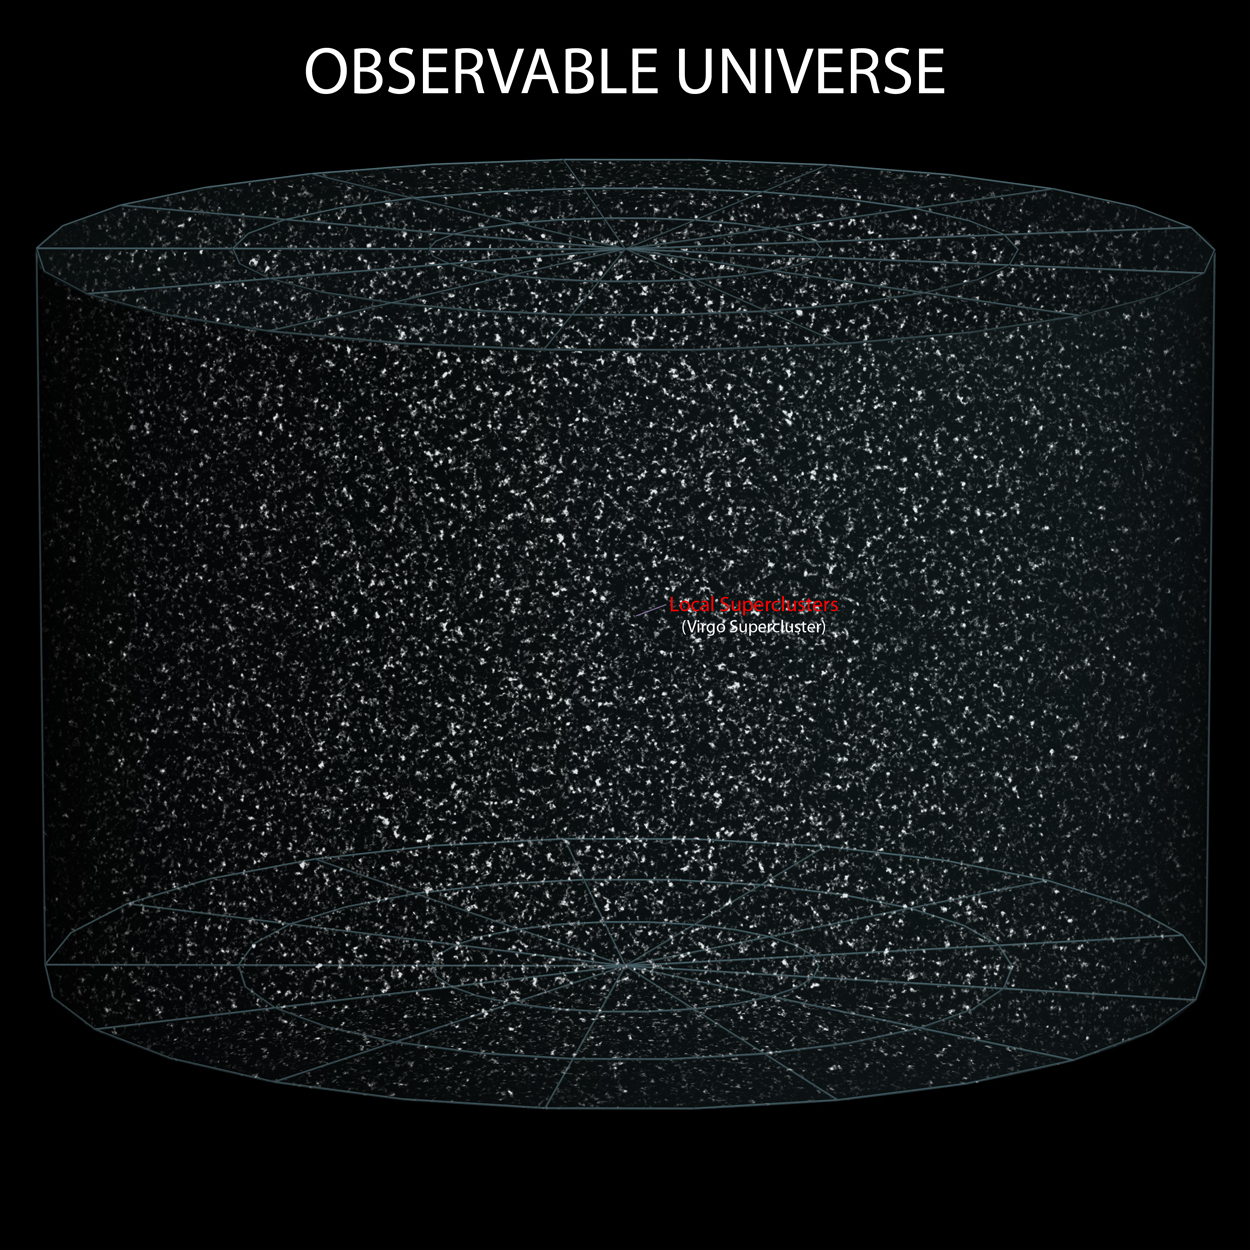
\includegraphics[width=\textwidth]{jwst/zoom_8.jpg}
        \column{0.49\textwidth}
        \begin{columns}
            \column{0.49\textwidth}
            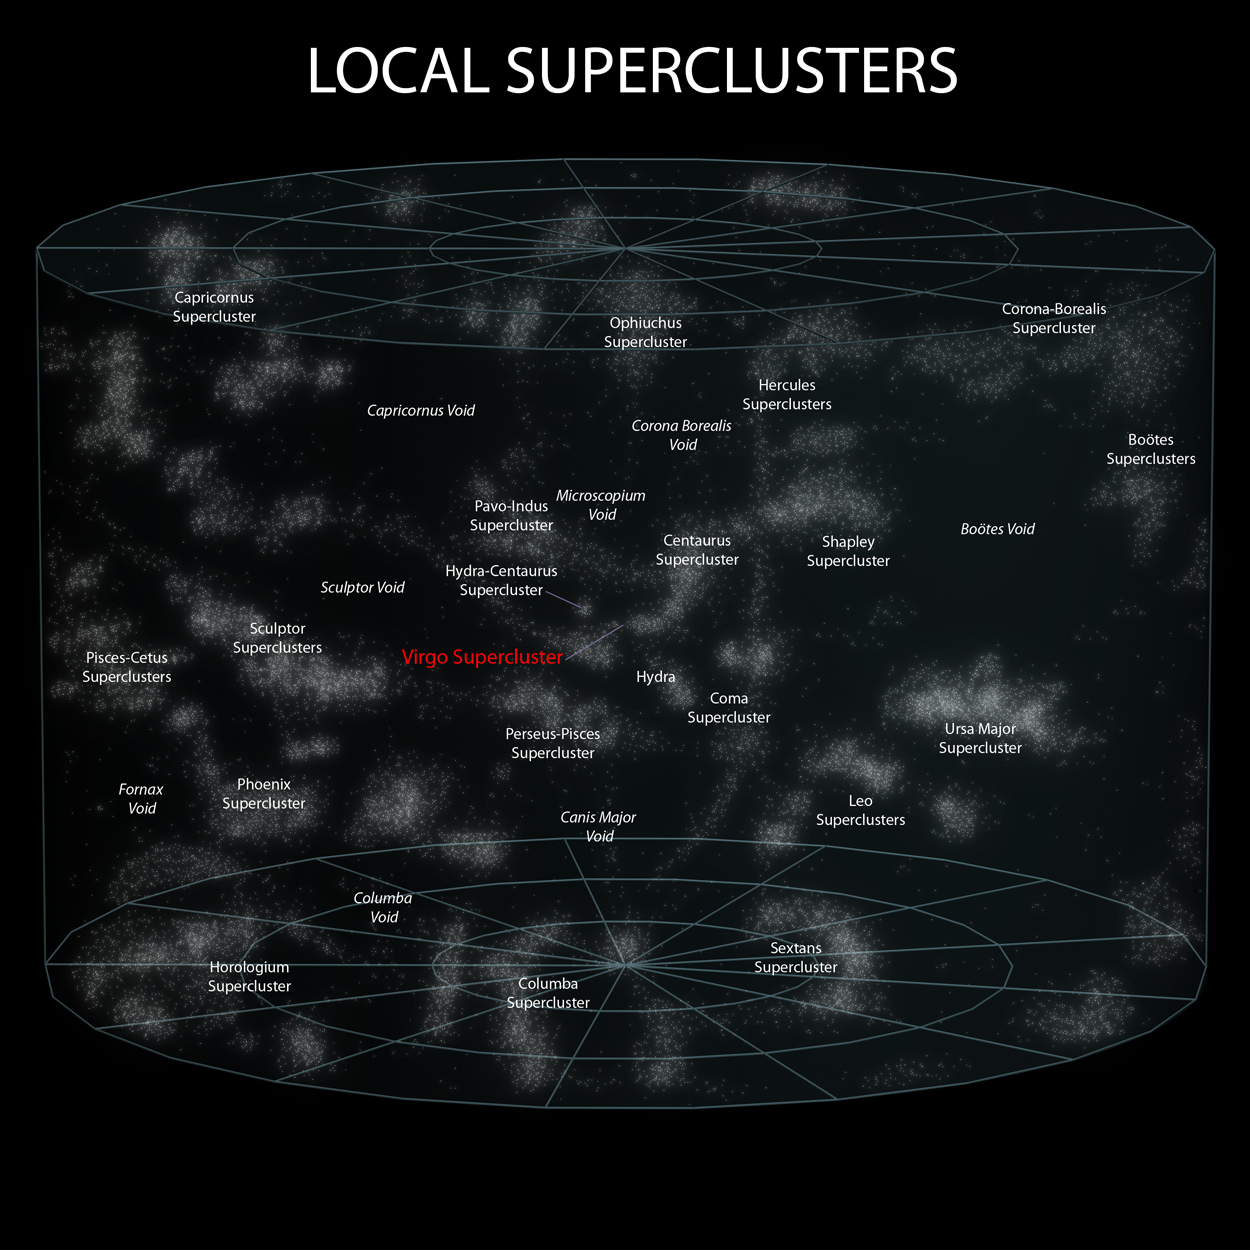
\includegraphics[width=\textwidth]{jwst/zoom_7.jpg}
            \column{0.49\textwidth}
            \begin{columns}
                \column{0.49\textwidth}
                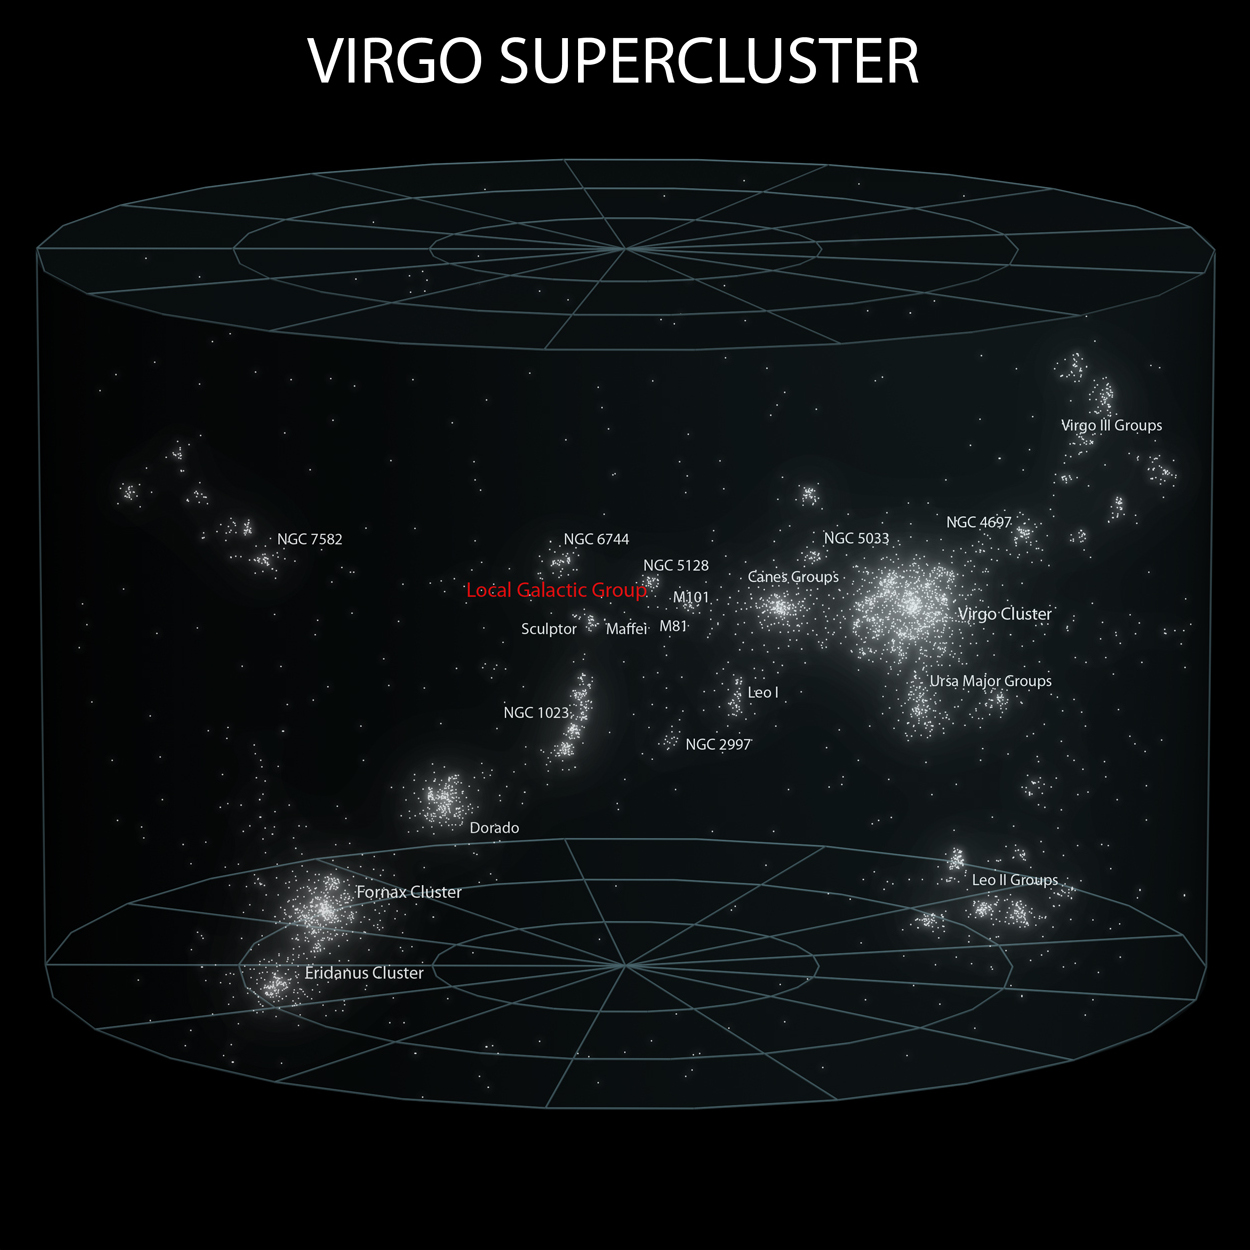
\includegraphics[width=\textwidth]{jwst/zoom_6.jpg}
                \column{0.49\textwidth}
                \begin{columns}
                    \column{0.49\textwidth}
                    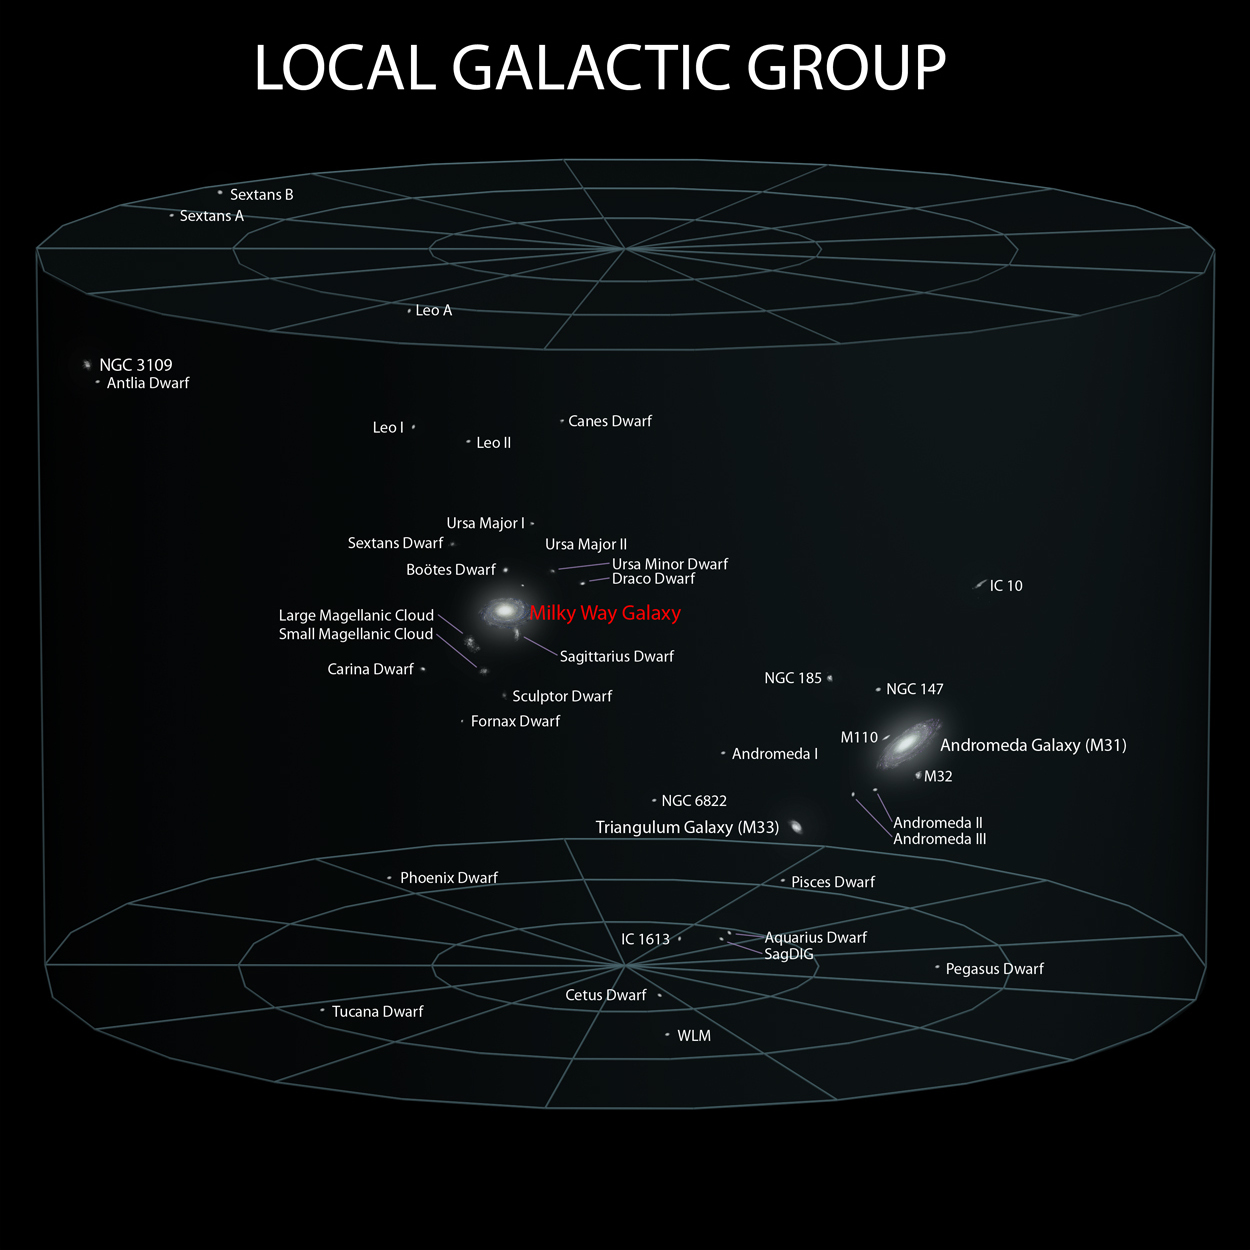
\includegraphics[width=\textwidth]{jwst/zoom_5.jpg}
                    \column{0.49\textwidth}
                    \begin{columns}
                        \column{0.49\textwidth}
                        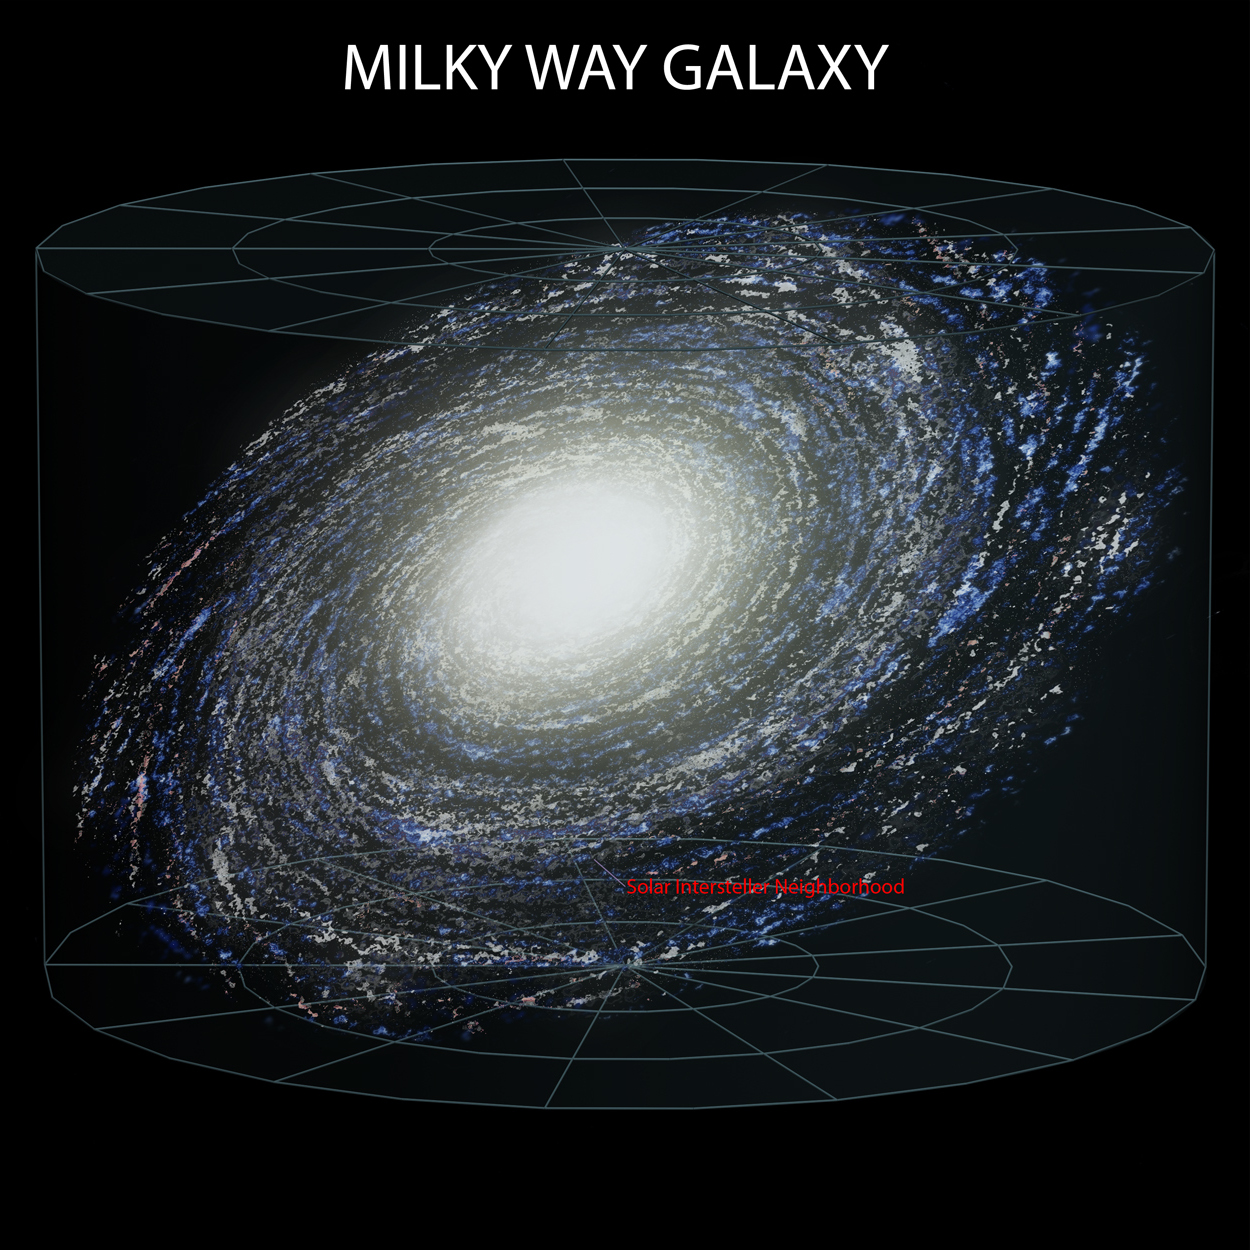
\includegraphics[width=\textwidth]{jwst/zoom_4.jpg}
                        \column{0.49\textwidth}
                        \begin{columns}
                            \column{0.49\textwidth}
                            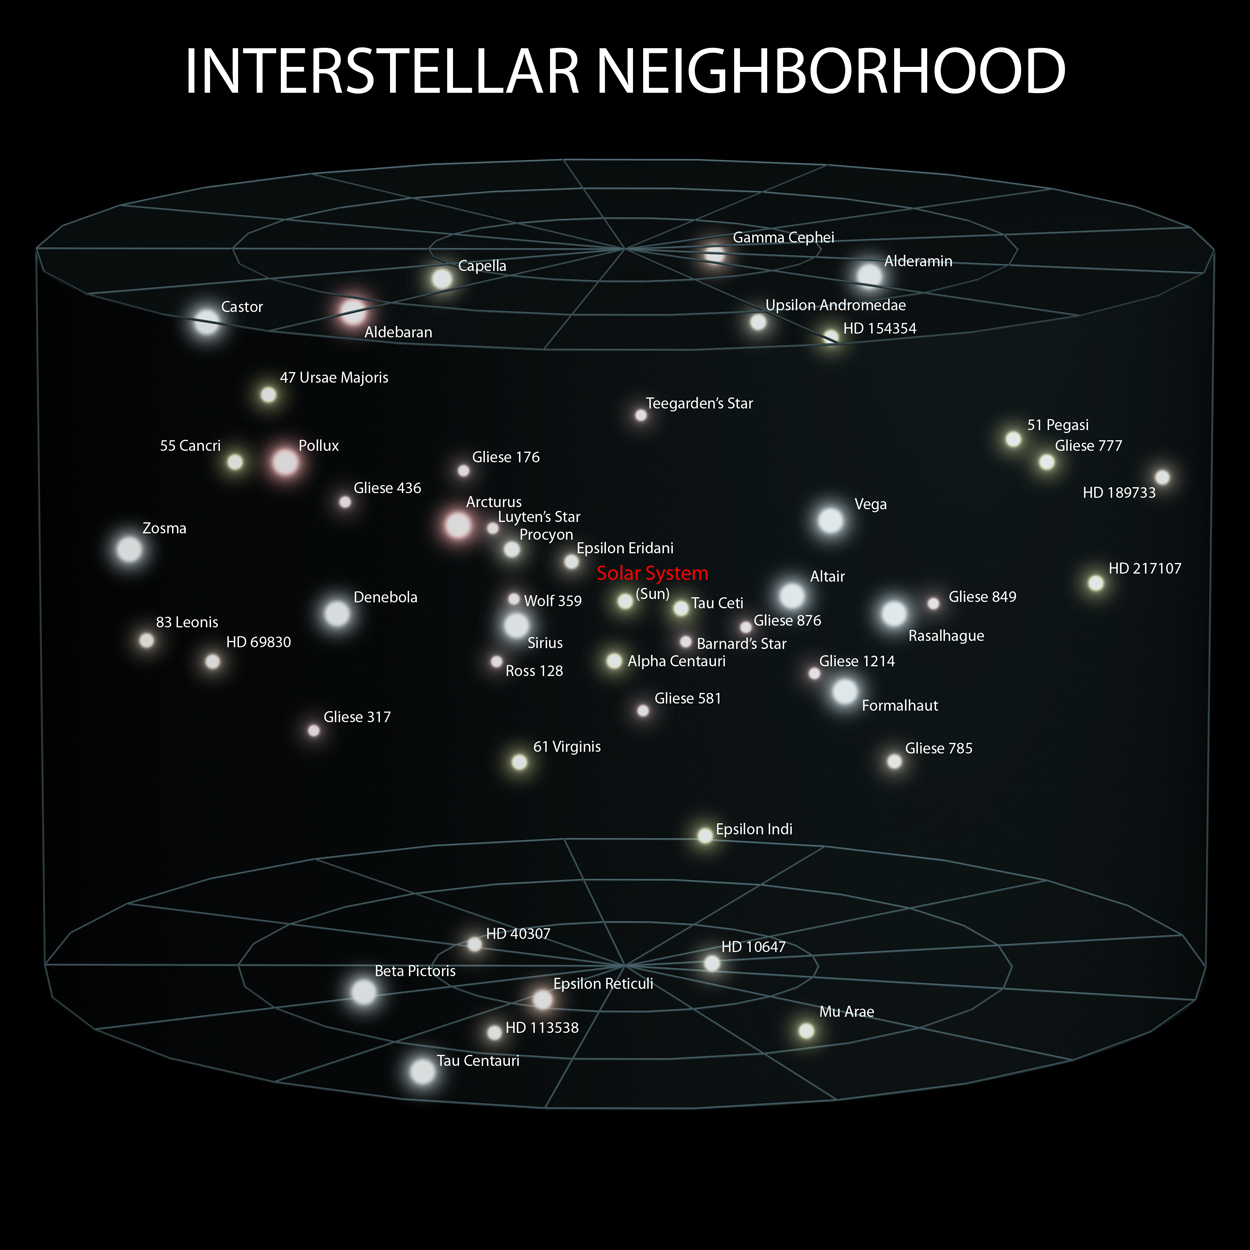
\includegraphics[width=\textwidth]{jwst/zoom_3.jpg}
                            \column{0.49\textwidth}
                            \begin{columns}
                                \column{0.49\textwidth}
                                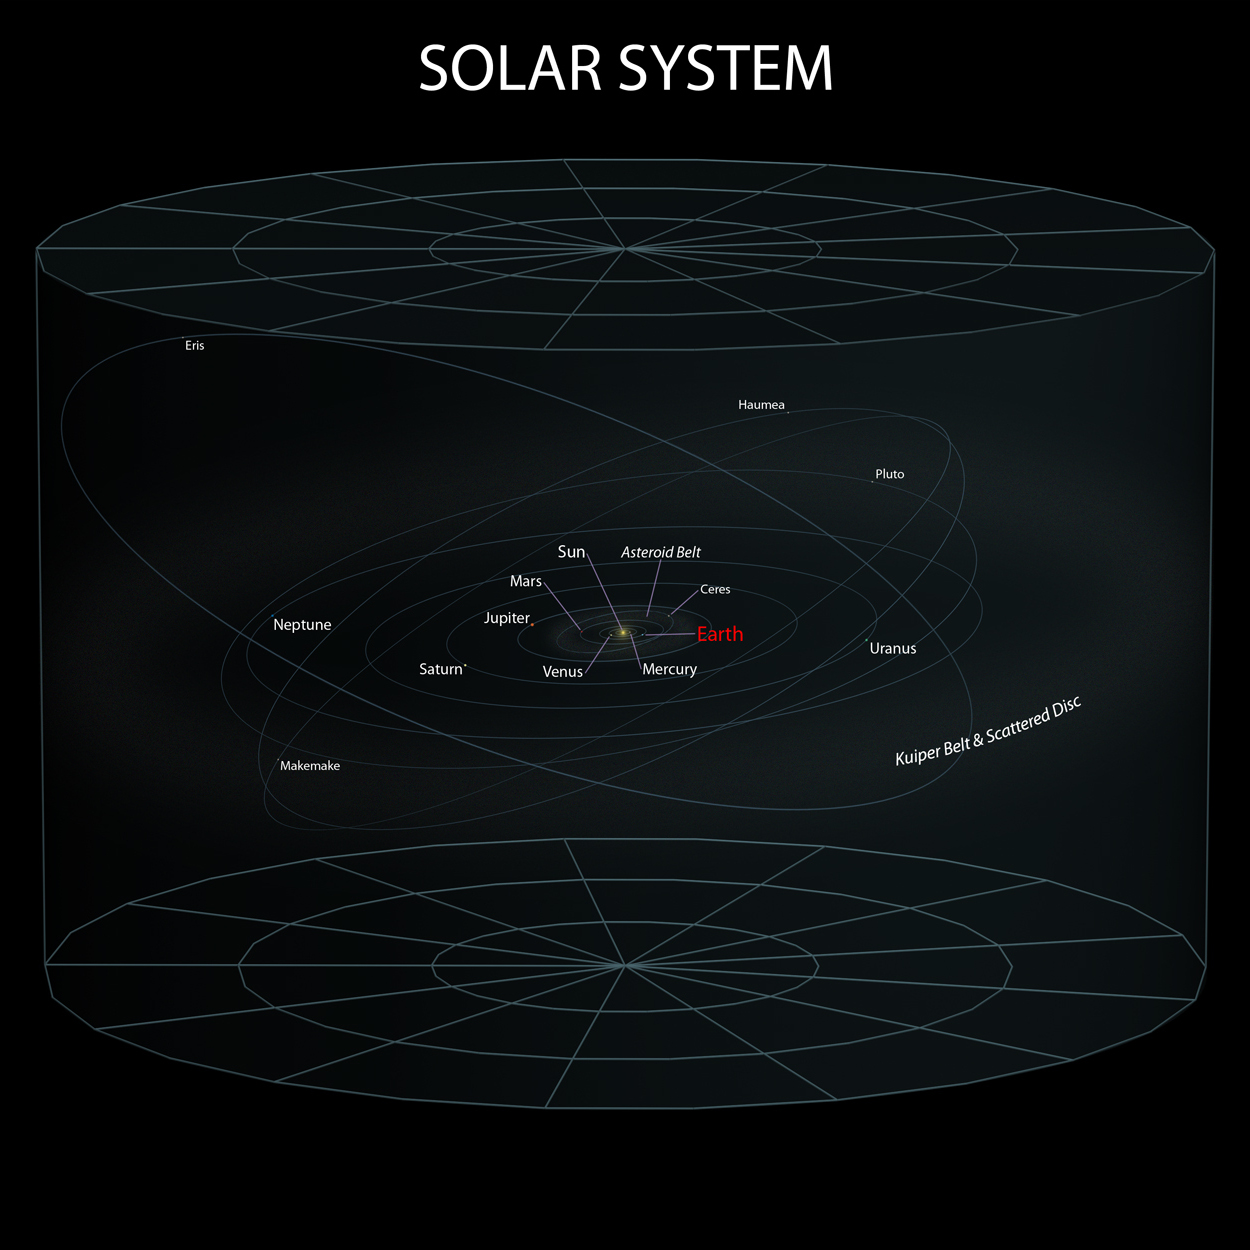
\includegraphics[width=\textwidth]{jwst/zoom_2.jpg}
                                \column{0.49\textwidth}
                                \begin{columns}
                                    \column{0.49\textwidth}
                                    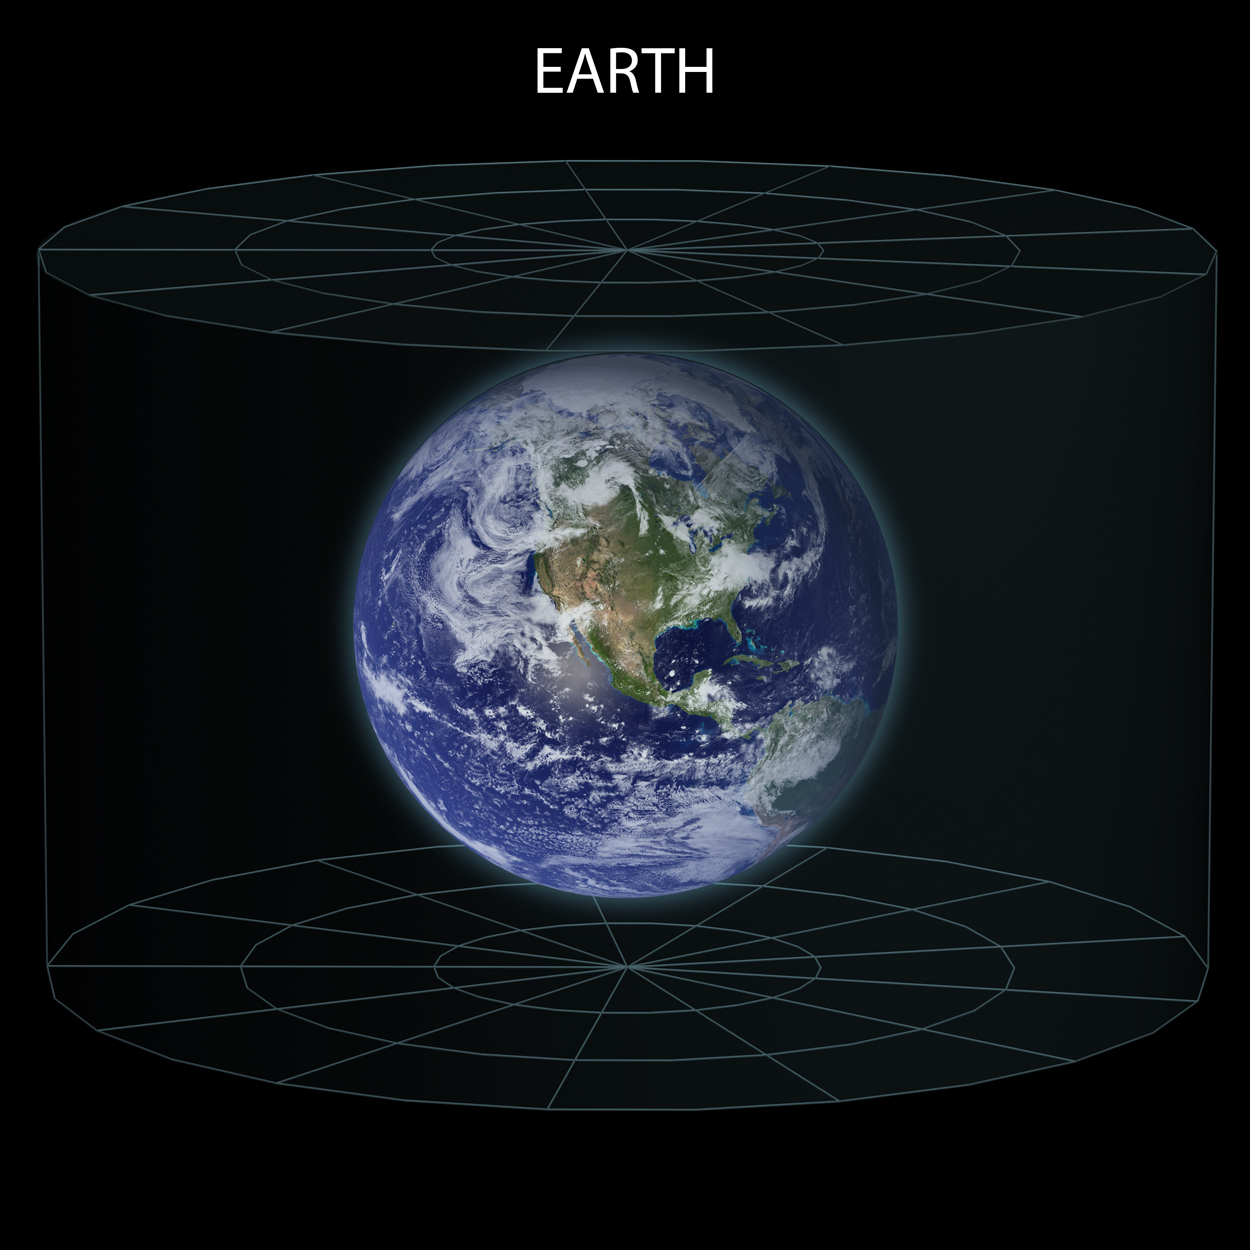
\includegraphics[width=\textwidth]{jwst/zoom_1.jpg}
                                    \column{0.49\textwidth}
                                \end{columns}
                            \end{columns}
                        \end{columns}
                    \end{columns}
                \end{columns}
            \end{columns}
        \end{columns}
    \end{columns}
\end{frame}

%\begin{frameb}{h}{Images/Milky_Way.jpg} 
%  \frametitle{The Night Sky}
%  \framesubtitle{The Milky Way}
%\end{frameb}
%
%\begin{frameb}{w}{Images/milky_way.jpg}
%\end{frameb}

\begin{frameb}{w}{CUPS/ESO-VLT-Laser-phot-33a-07.jpg} 
  \frametitle{Ground Based Telescopes}

  \makebox[\textwidth][c]{%
    \begin{tikzpicture}
      \node<1-> at (0,0) {};
      \node<2-> (rect) at (-11,5) [draw,thick,minimum width=0.5cm,minimum height=0.5cm] {};
    \end{tikzpicture}
  }
\end{frameb}

%\begin{frameb}{w}{Images/Coma_Cluster.jpg} 
%  \frametitle{Ground based telescopes}
%  \framesubtitle{The Coma Cluster}
%\end{frameb}
%
%\plainframe{
	\movie[width=\textwidth,height=\textheight]{}{Movies/sdss_flythrough.avi}	
	}





\begin{frameb}{w}{CUPS/Pandora’s_Cluster_(Abell_2744)_Uncover_program.png}
  \frametitle{Space based telescopes}

  \makebox[\textwidth][c]{%
    \begin{tikzpicture}
      \node<1-> at (0,0) {};
      \node<2-> (rect) at (9.5,5.5) [draw,thick,minimum width=0.5cm,minimum height=0.5cm] {};
    \end{tikzpicture}
  }
\end{frameb}


\begin{frameb}{w}{CUPS/Hubble.png} 
  \frametitle{Hubble deep field}
\end{frameb}

\begin{frameb}{w}{CUPS/Webb.png} 
  \frametitle{James Webb deep field}
  \makebox[\textwidth][c]{%
    \begin{tikzpicture}
      \node<1-> at (0,0) {};
      \node<2-> (rect) at (+1,+6.6) [draw,thick,minimum width=0.5cm,minimum height=0.5cm] {};
    \end{tikzpicture}
  }
\end{frameb}

\begin{frame}
  \frametitle{The Dark Ages}
  \makebox[\textwidth][c]{%
    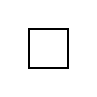
\begin{tikzpicture}
      \node<1-> at (0,0) {};
      \node<2-> (rect) at (0,0) [draw,thick,minimum width=0.5cm,minimum height=0.5cm] {};
    \end{tikzpicture}
  }
\end{frame}

{%
  \definecolor{cmbcolour}{RGB}{120,120,120}	    
  \setbeamercolor{background canvas}{bg=cmbcolour}
  \begin{frame}
    \frametitle{The Cosmic Microwave Background}
  \end{frame}
}
\begin{frameb}{w}{Images/wmap_cmb.png} 
    \frametitle{The Cosmic Microwave Background: WMAP}
\end{frameb}
\begin{frameb}{w}{Images/planck_cmb.png} 
    \frametitle{The Cosmic Microwave Background: Planck}
\end{frameb}
\begin{frameb}{w}{Images/spt_cmb.png} 
    \frametitle{The Cosmic Microwave Background: ACT/SPT}
\end{frameb}

%\begin{frameb}{w}{Images/Hubble_Ultra_Deep_Field_diagram.jpg}
\begin{frameb}{w}{CUPS/STScI-01EVT7KBK7M9JWVTA7AY9TCW0W.jpg}
\end{frameb}

\begin{frame}
    \frametitle{Summary of observations}
    \begin{columns}
        \column{0.5\textwidth}
        \begin{itemize}
            \item See ``epoch shells'' of the universe.
            \item Time-delayed light arrives from across cosmic history onto our night sky.
            \item An evolving, expanding universe.
            \item Beginning: a hot, dense, infinite spatial soup of matter and energy.
            \item Evolution: expanding and cooling across history of 13.8 billion years,
            \item Gravity collapses matter out of this cosmic flow into clusters, galaxies, planets and people.
        \end{itemize}
        \column{0.5\textwidth}
        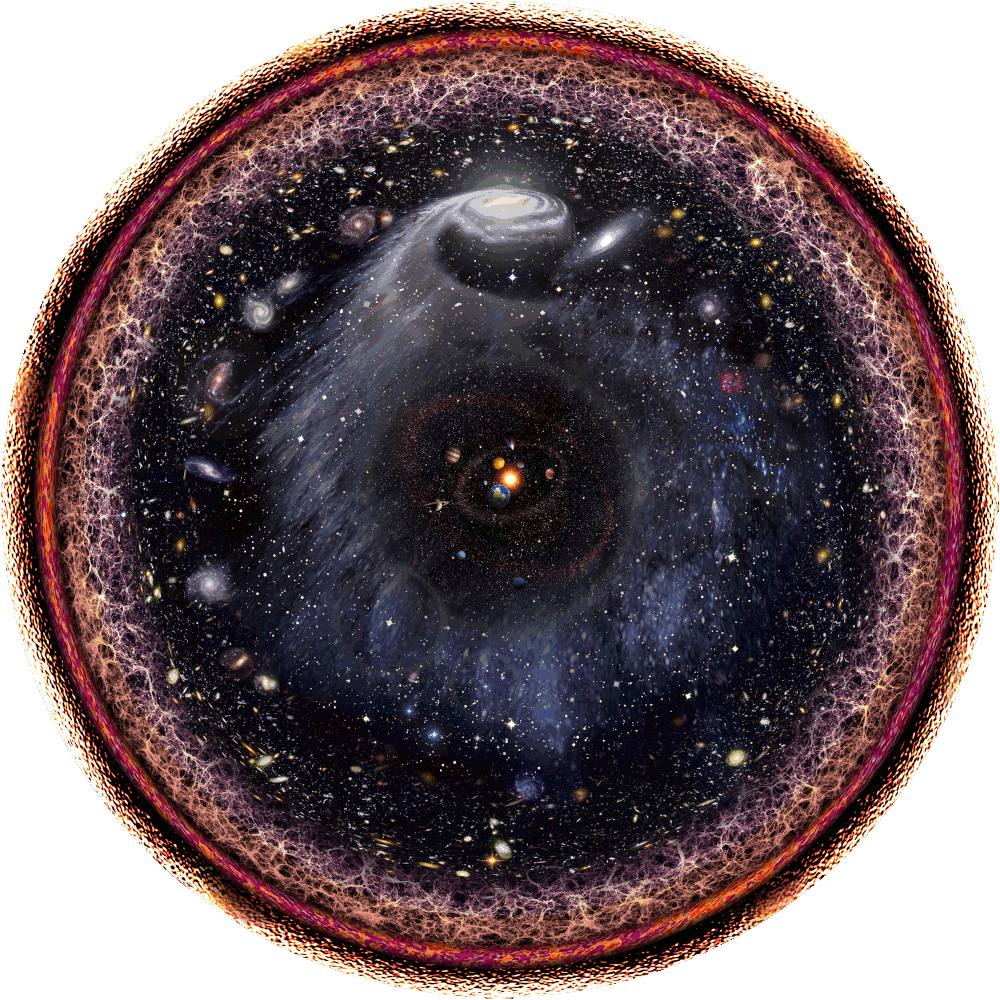
\includegraphics[width=\textwidth]{RAC/modern}
    \end{columns}
\end{frame}

%\begin{frame}
%    \frametitle{Hubble vs Webb}
%    \begin{columns}
%        \column{0.3\textwidth}
%        
%        \column{0.7\textwidth}
%        \vspace{-30pt}
%        \includegraphics<1>[width=\textwidth]{CUPS/Hubble.png}%
%        \includegraphics<2>[width=\textwidth]{CUPS/Webb.png}
%    \end{columns}
%    <++>
%\end{frame}

%\begin{frame}
%    \frametitle{Disclaimers}
%    \begin{itemize}
%        \item I am not on the JWST team
%            \begin{itemize}
%                \item like every astronomer it will continue to have a large impact for many decades
%            \end{itemize}
%        \item JWST has been taking images for half a year now, but only a fraction of them are public
%        \item This talk is designed to give you a framework to interpret any news stories
%        \item Hope for a more new-science focussed talk next year.
%        \item Structure of talk
%            \begin{enumerate}
%                \item Orienting our place in the universe
%                \item Description of the JWST observatory
%                \item Discussion of the science it is interested in
%                \item Latest pictures from JWST
%            \end{enumerate}
%    \end{itemize}
%\end{frame}

\begin{frame}
    \frametitle{The Big Bang theory}

    \begin{columns}
        \column{0.5\textwidth}
        To follow our cosmogeny, you need to understand the answers to these questions:

        \begin{enumerate}
            \item When did the Big Bang happen?
                \begin{itemize}
                    \item<2-> 14 billion years ago
                \end{itemize}
            \item Where did the Big Bang happen?
                \begin{itemize}
                    \item<3-> Everywhere
                \end{itemize}
            \item What is the Universe expanding into?
                \begin{itemize}
                    \item<4-> Itself
                \end{itemize}
            \item What happened before the Big Bang
                \begin{itemize}
                    \item<5-> There was no before
                \end{itemize}
            \item Why did the Big Bang happen?
                \begin{itemize}
                    \item<6-> Observations cannot tell us \onslide<7->{(yet)}
                \end{itemize}
        \end{enumerate}

        \column{0.5\textwidth}
        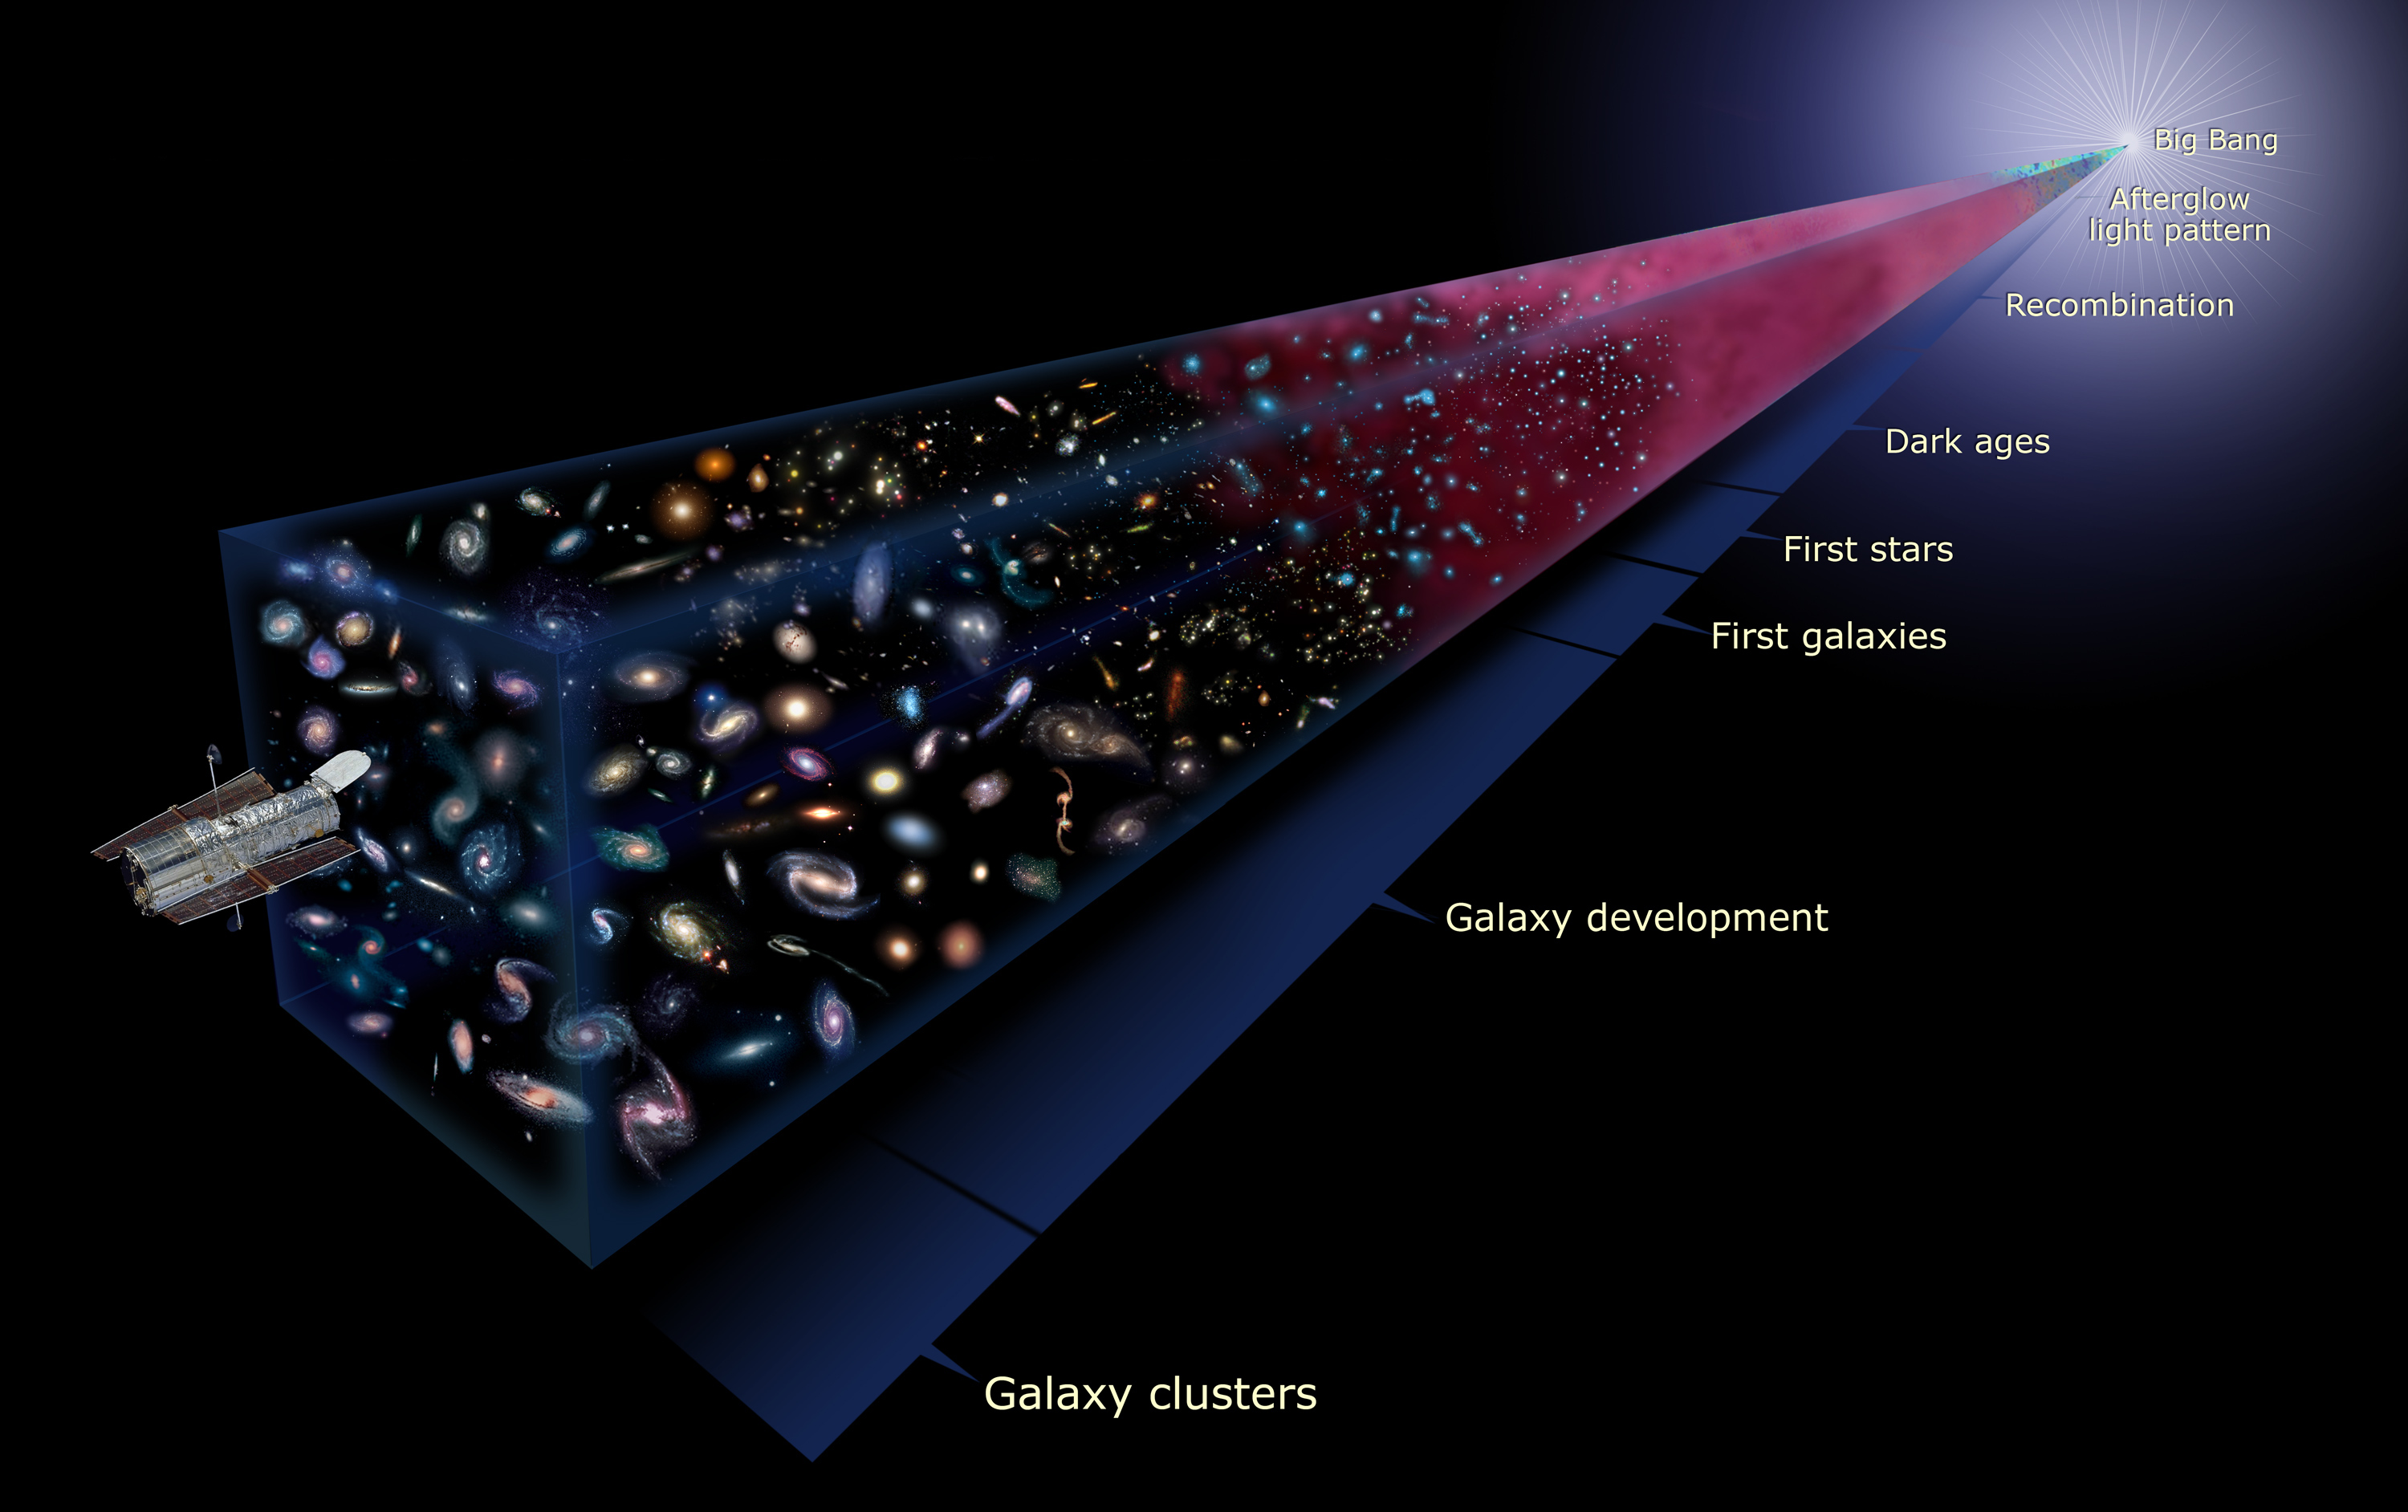
\includegraphics[width=\textwidth]{CUPS/STScI-01EVT7KBK7M9JWVTA7AY9TCW0W.jpg}
        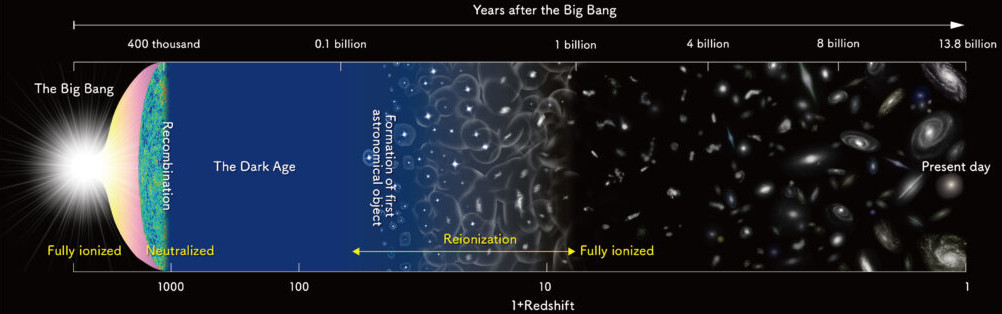
\includegraphics[width=\textwidth]{RAC/timeline-1024x369.jpg}
    \end{columns}
\end{frame}

\begin{frame}[label=current]
    \frametitle{Modelling the Universe}
    \begin{columns}[b]
        \column{0.5\textwidth}
        In general need to describe:
        \begin{enumerate}
            \item Content
            \item Size and shape
            \item Initial conditions and evolution
        \end{enumerate}
        \pause
        \column{0.5\textwidth}
        The $\Lambda$CDM concordance model:
        \begin{enumerate}
            \item (Dark) matter and radiation
            \item Flat, homogenous and isotropic
            \item Evolution dictated by Einstein's GR
        \end{enumerate}
    \end{columns}
    \vspace{10pt}

    \pause
    \begin{columns}
        \column{0.6\textwidth}
        $\Lambda$CDM introduces six unknown quantities:
        \pause
        \begin{itemize}
            \item<4-> Constituents: 
                \begin{enumerate}
                    \item<5-> Fraction of Visible ``baryonic matter'' $\Omega_b$
                    \item<6-> Fraction of ``cold'' Dark matter $\Omega_c$
                    \item<7-> Cloudiness (optical depth) to the CMB $\tau$
                \end{enumerate}
            \item<4-> Scale and shape
                \begin{enumerate}\addtocounter{enumi}{3}
                    \item<8-> Present day expansion rate: $H_0$
                \end{enumerate}
            \item<4-> Initial conditions:
                \begin{enumerate}\addtocounter{enumi}{4}
                    \item<9-> Amplitude of primordial fluctuations $A_s$
                    \item<10-> Spectral index of primordial fluctuations $n_s$
                \end{enumerate}
        \end{itemize}
        \column{0.4\textwidth}
        \begin{itemize}
            \item<11-> From these flow a host of derived quantities, such as:
                Dark energy $\Omega_\Lambda$,
                Radiation $\Omega_r$,
                Neutrinos $\Omega_\nu$.
            \item<12-> Any of these can be extended/adjusted/removed and tested against data
        \end{itemize}
    \end{columns}
\end{frame}
%mmHg      kg m^-1 s^-2 
%megatonne kg m^2  s^-1
%mmHg/megatonne concentration 


\begin{frame}[label=current]
    \frametitle{Measuring $H_0$}
        \begin{itemize}
            \item University challenge question: In what units is the Hubble constant measured?
            \pause
            \begin{itemize}
                \item km s$^{-1}$/ Mpc
            \end{itemize}
            \pause
            \item recession speed / distance
            \item Just need to measure:
                \begin{enumerate}
                    \item How fast objects are moving away (redshift)
                    \item How far away those objects are
                \end{enumerate}
            \item The second of these is the challenging one!
            \item Three methods:
                \pause
                \begin{enumerate}
                    \item Standard candles
                    \item Standard rulers
                    \item Standard sirens
                \end{enumerate}

        %\item If $H_0=100$, then 
        %    \begin{itemize}
        %        \item objects 1 Mpc away are moving at 100 kms$^{-1}$ 
        %        \item objects 0.1 Mpc away are moving at 10 kms$^{-1}$ 
        %        \item objects 10 Mpc away are moving at 1000 kms$^{-1}$
        %    \end{itemize}
        %    \pause
        \end{itemize}
\end{frame}

\begin{frame}[label=current]
    \frametitle{Standard candles}
    \begin{columns}
        \column{0.45\textwidth}
        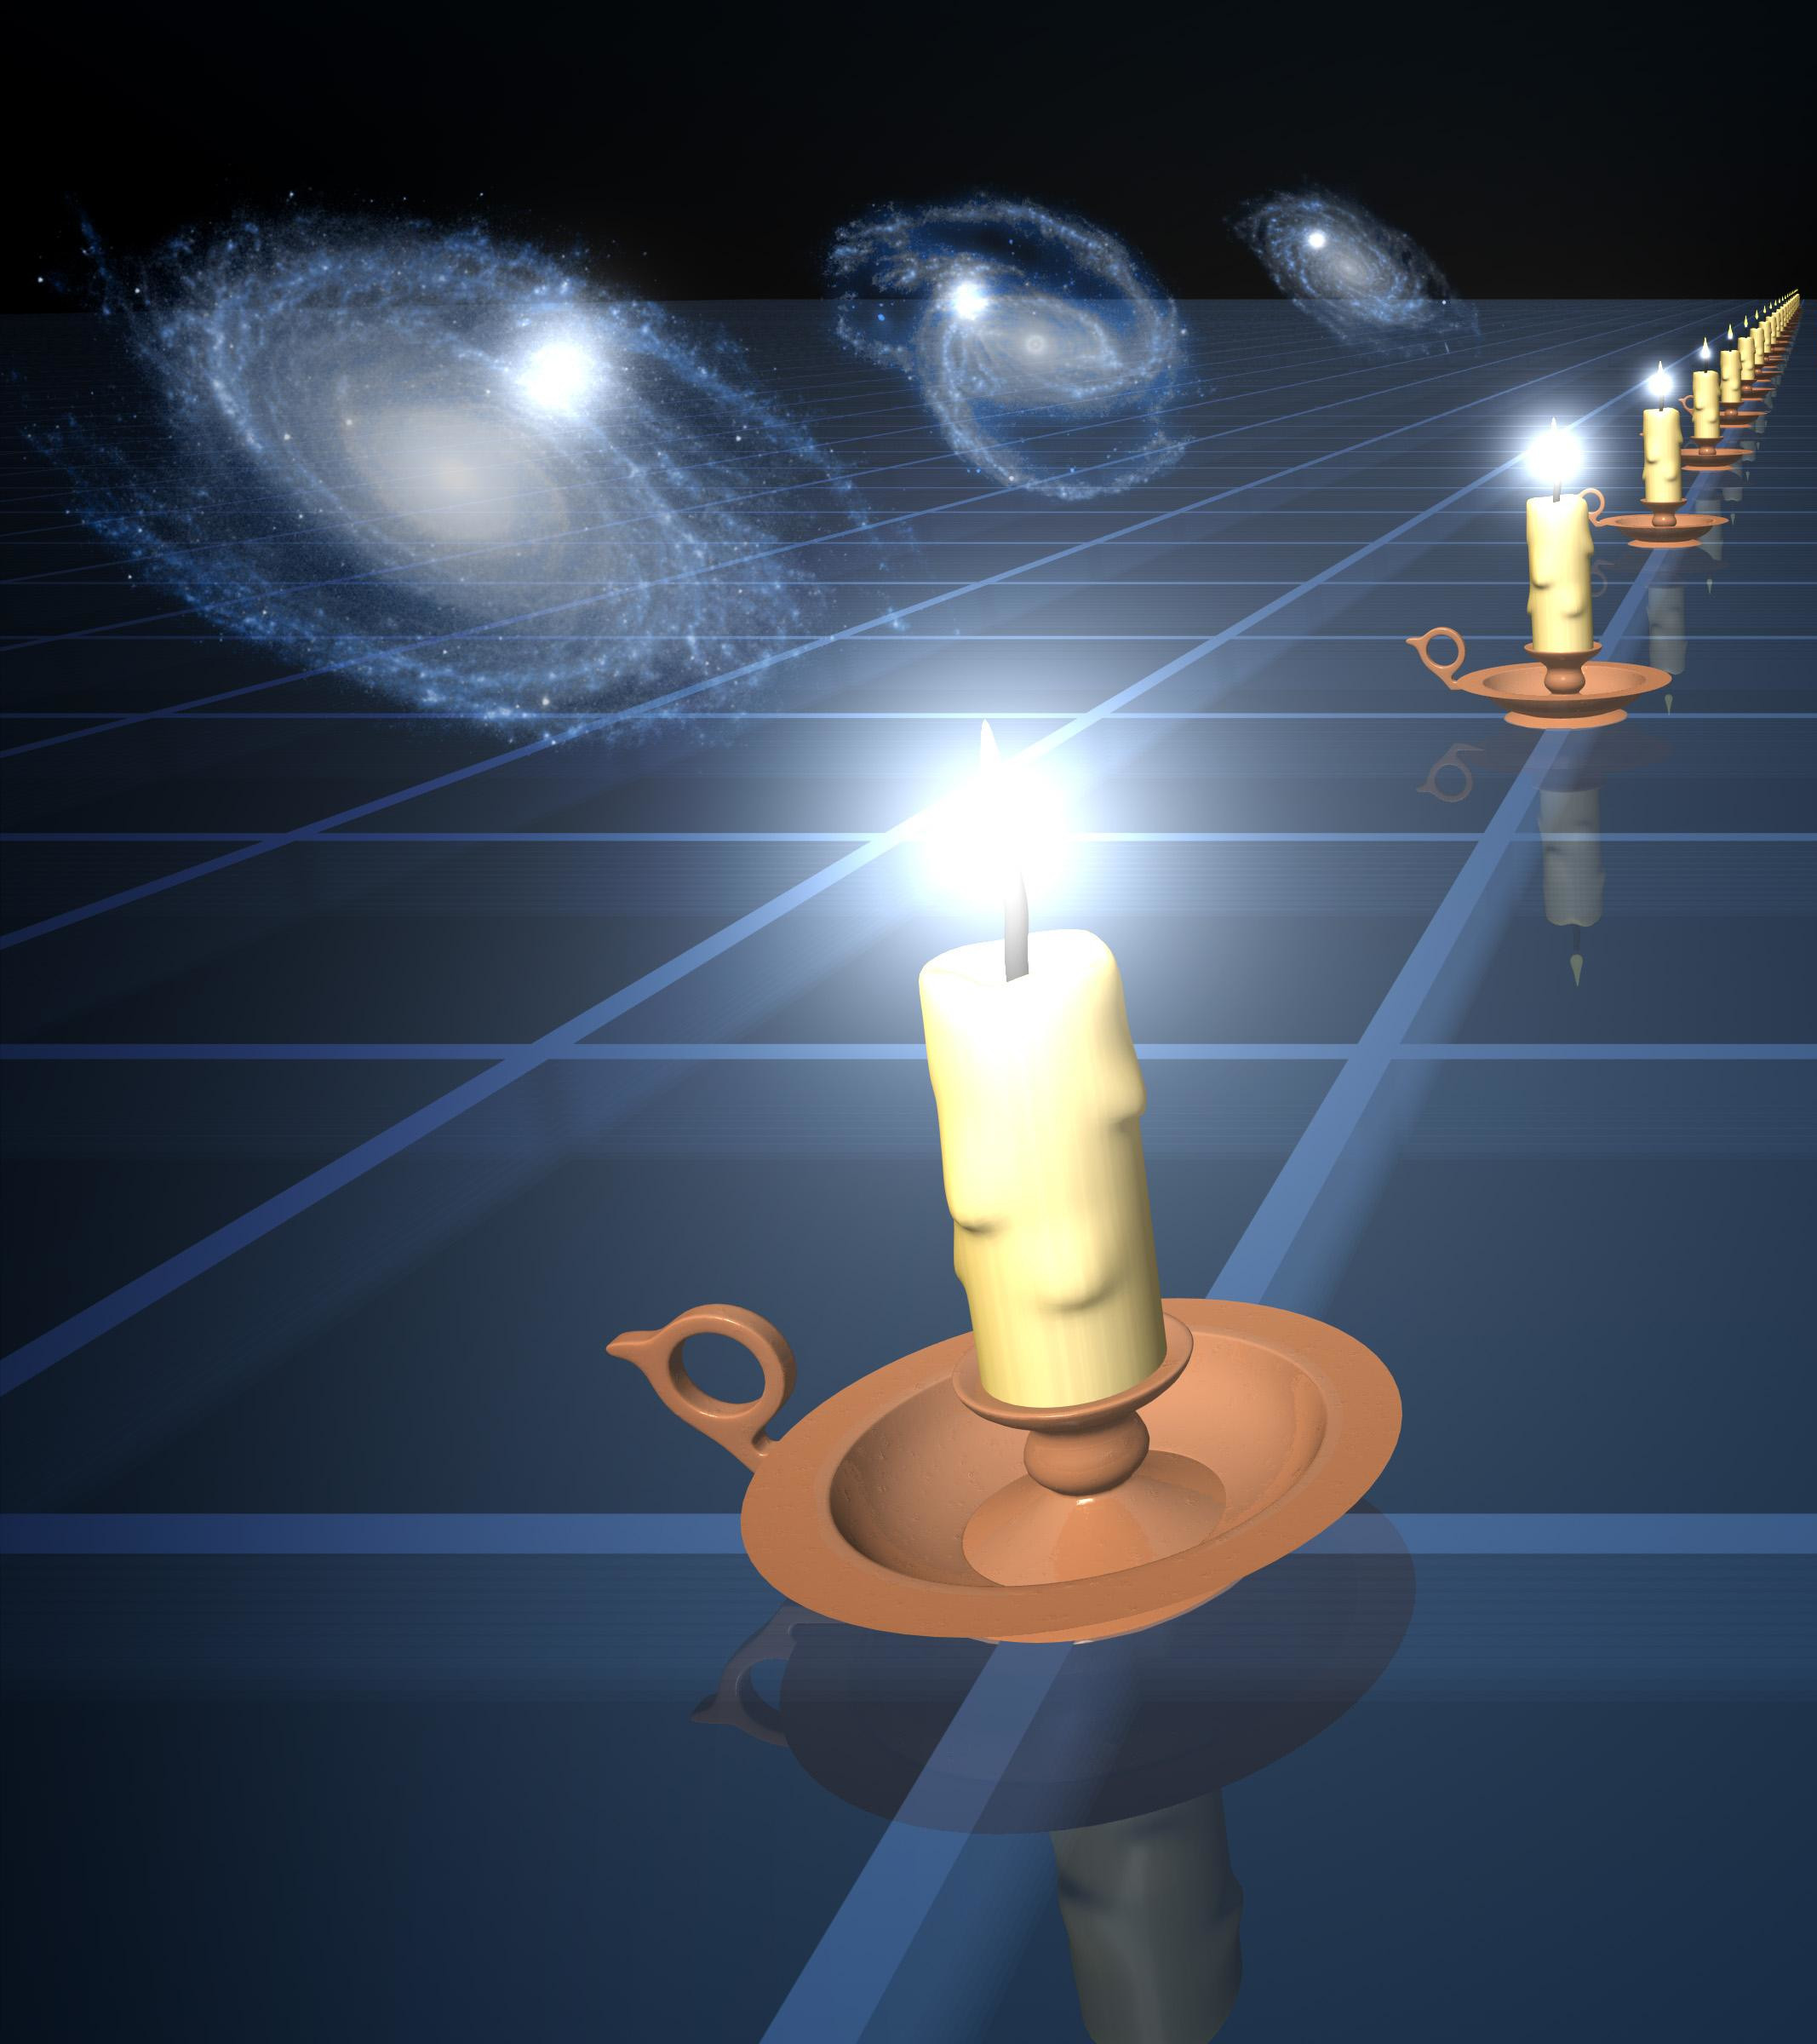
\includegraphics[width=\textwidth]{CUPS/candles.jpg}
        \column{0.55\textwidth}
        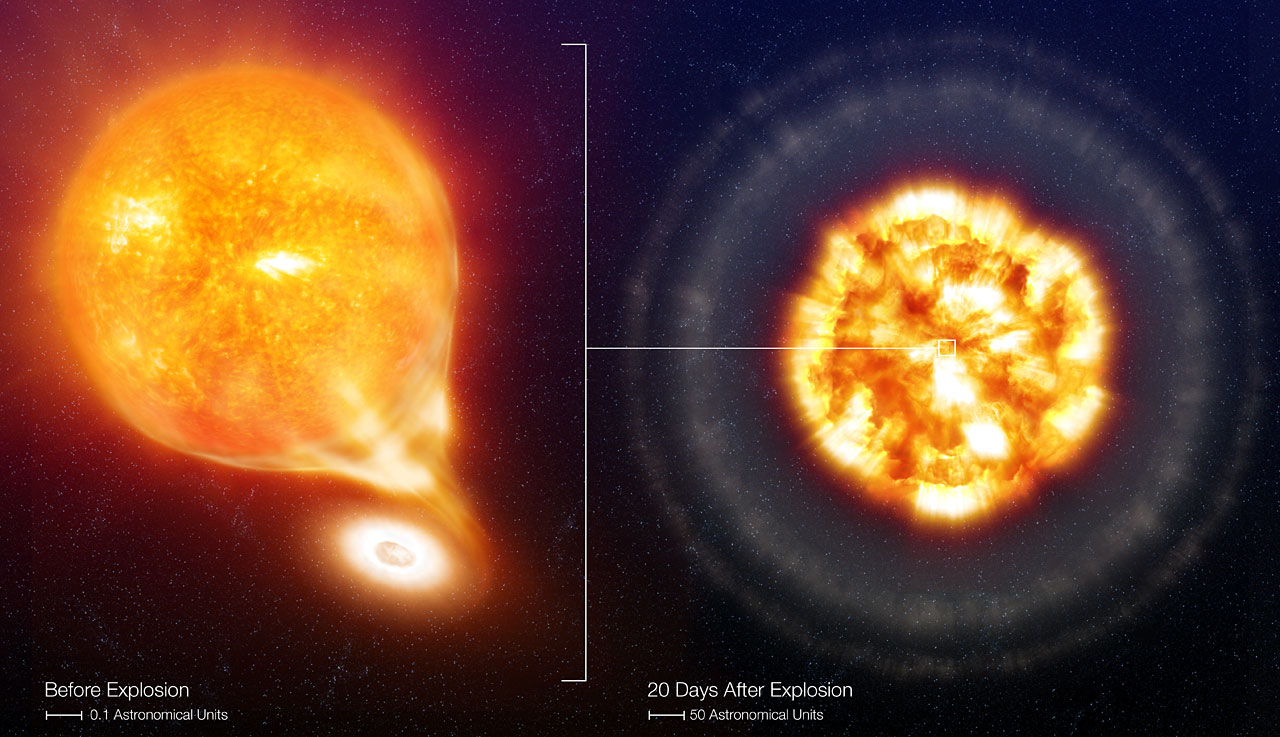
\includegraphics[width=\textwidth]{CUPS/eso0731b.jpg}
        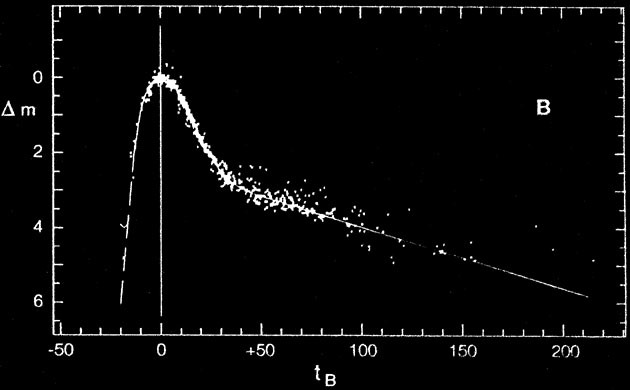
\includegraphics[width=0.49\textwidth]{CUPS/sne.jpeg}
        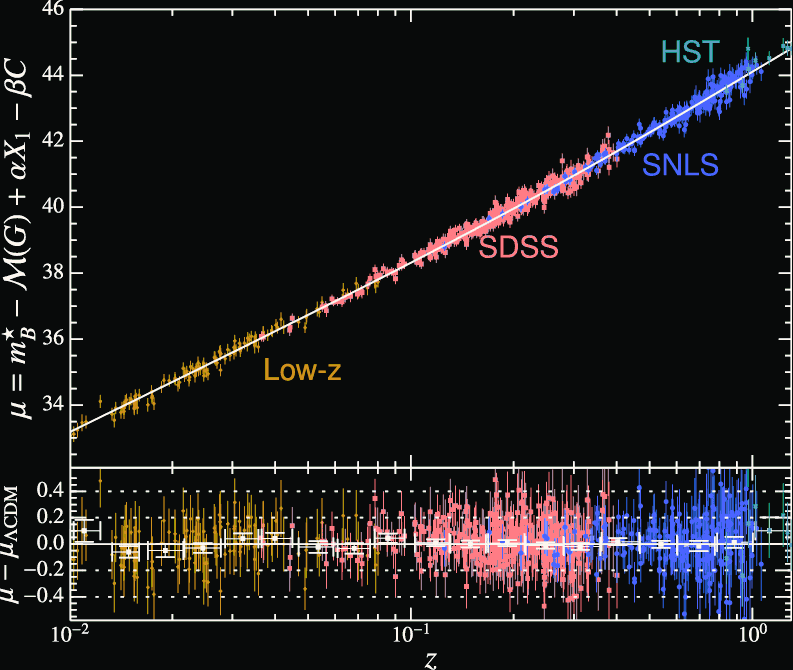
\includegraphics[width=0.49\textwidth]{CUPS/hubble_diagram.png}
    \end{columns}
\end{frame}

\begin{frame}[label=current]
    \frametitle{Standard rulers}
    \begin{columns}
        \column{0.45\textwidth}
        \only<1>{
            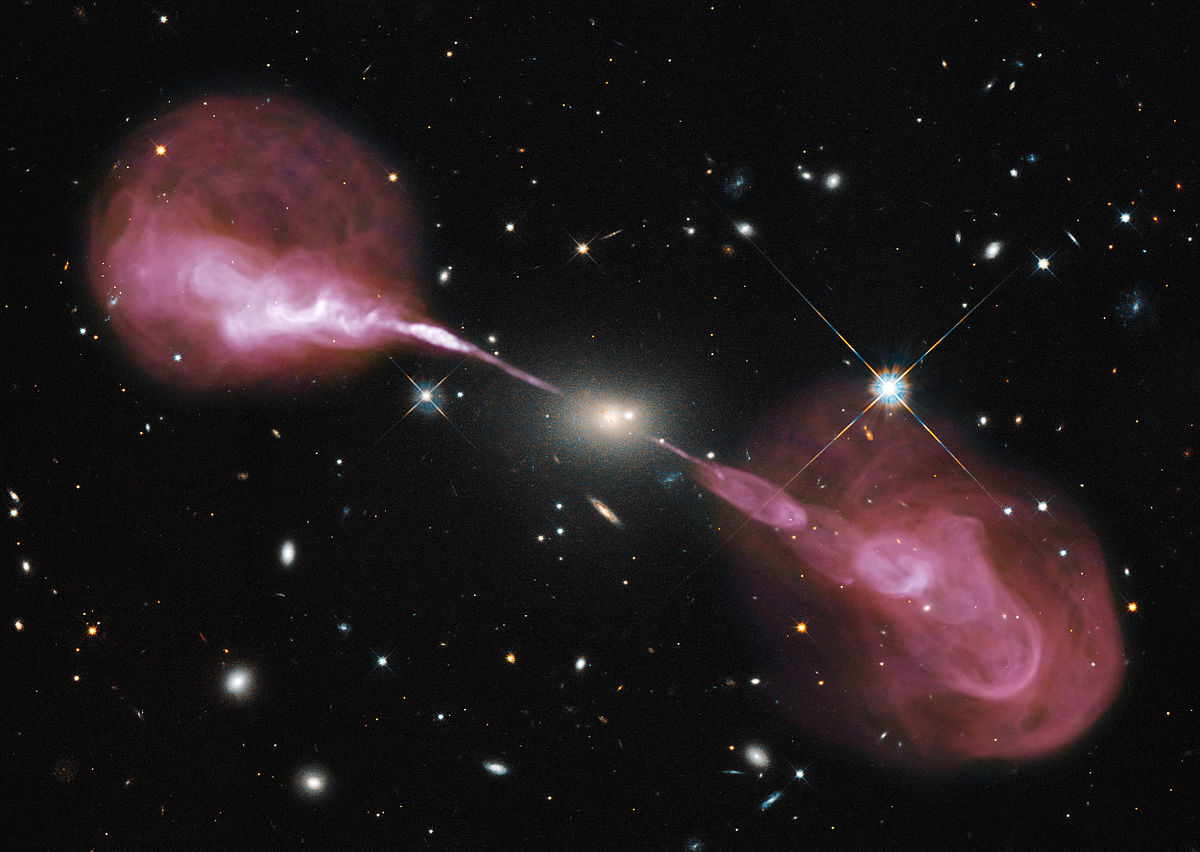
\includegraphics[width=0.75\textwidth]{CUPS/1200px-A_Multi-Wavelength_View_of_Radio_Galaxy_Hercules_A.jpg}%

            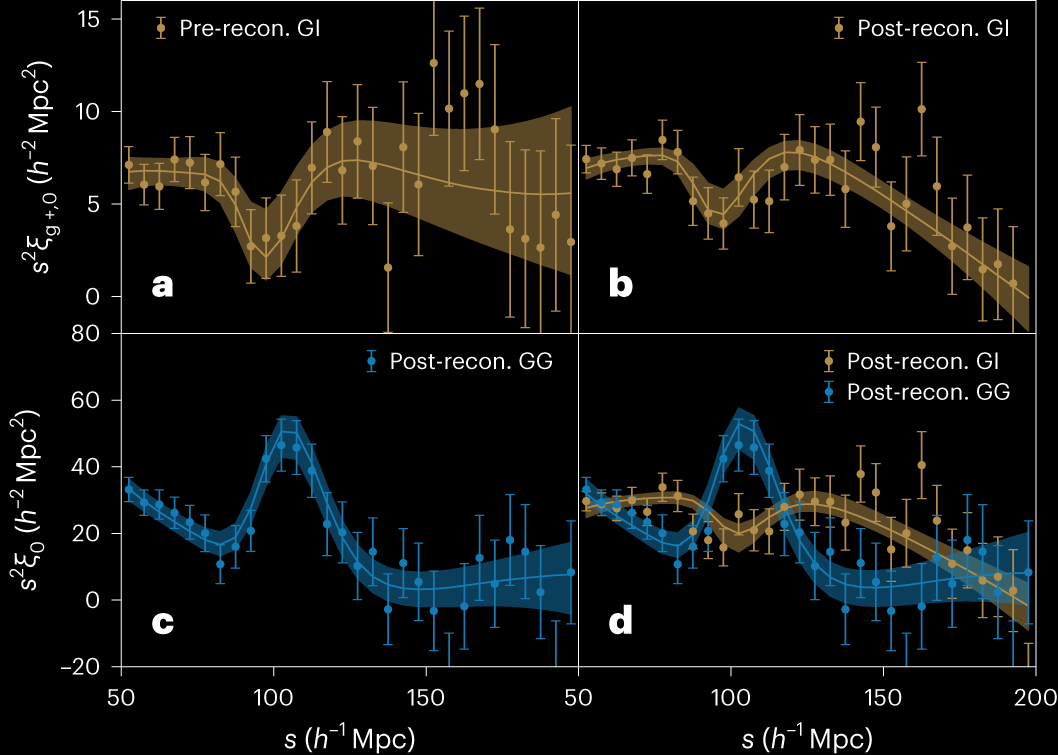
\includegraphics[width=0.75\textwidth]{CUPS/bao.png}%
        }%
        \only<2->{
            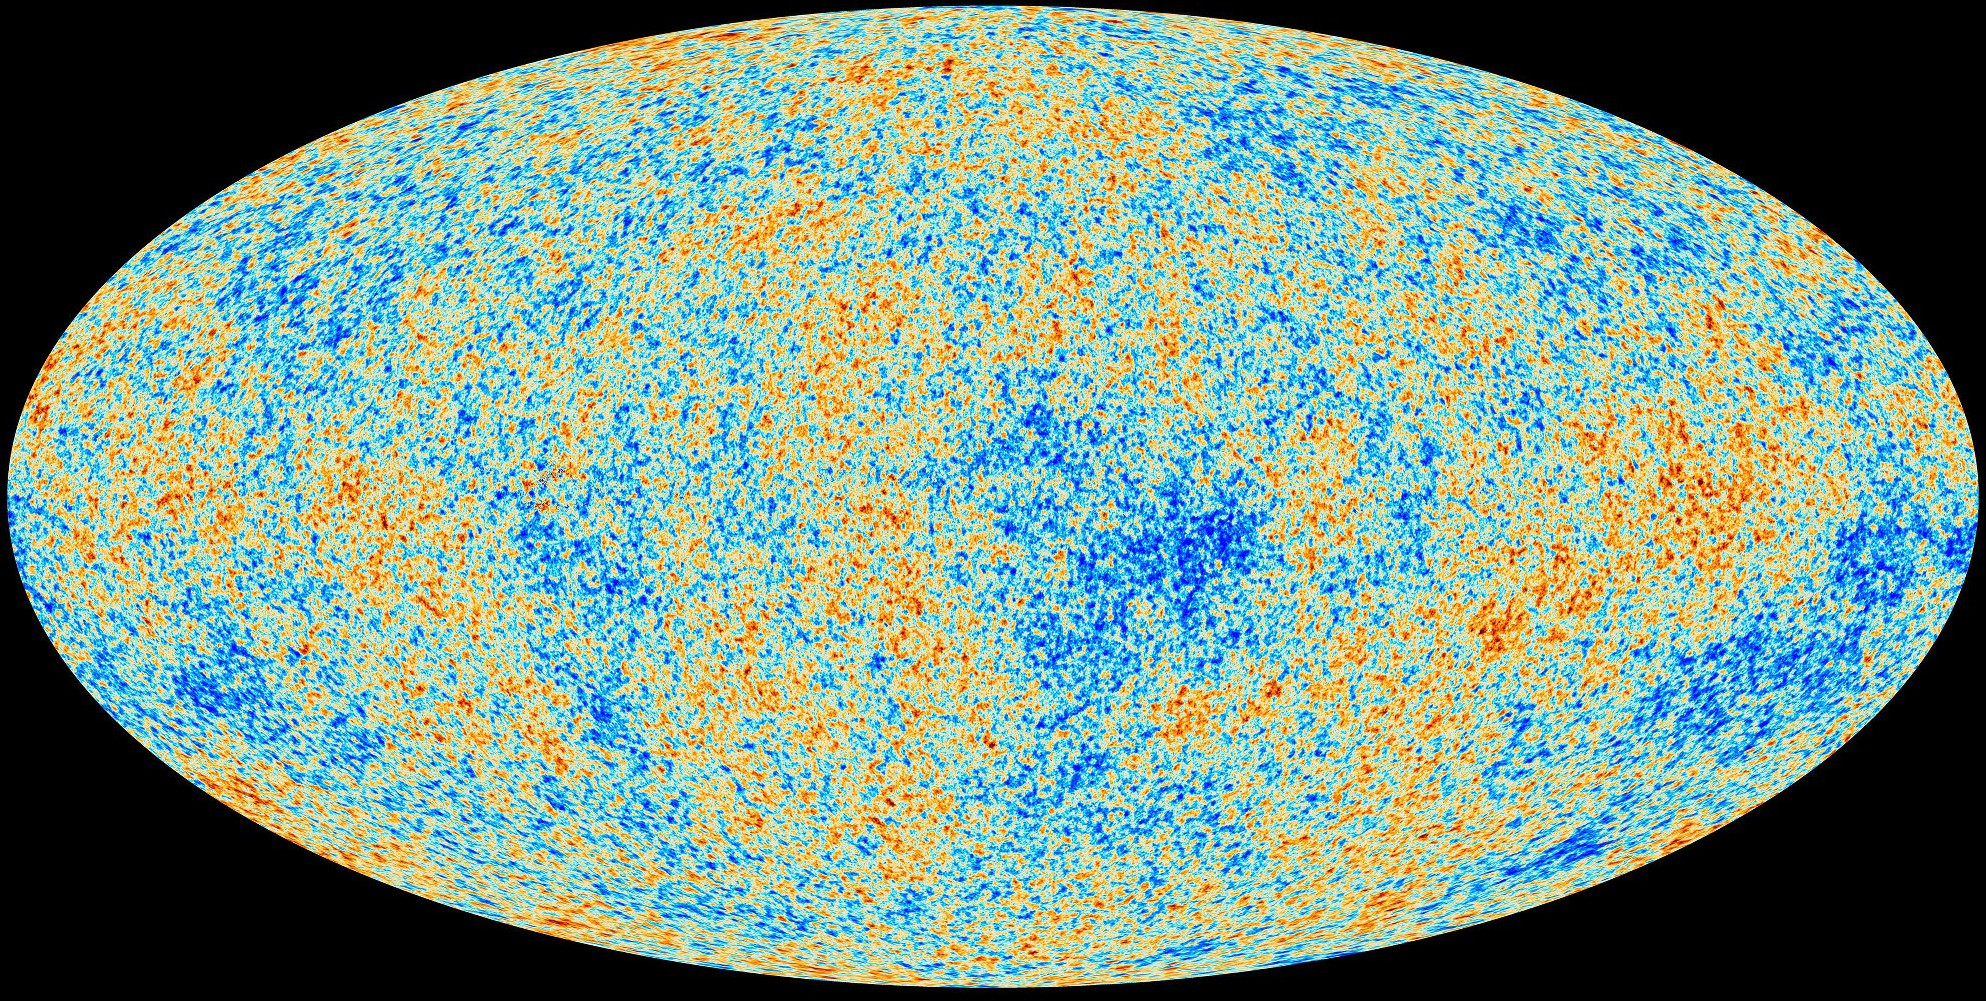
\includegraphics[width=\textwidth]{Images/planckdata}
            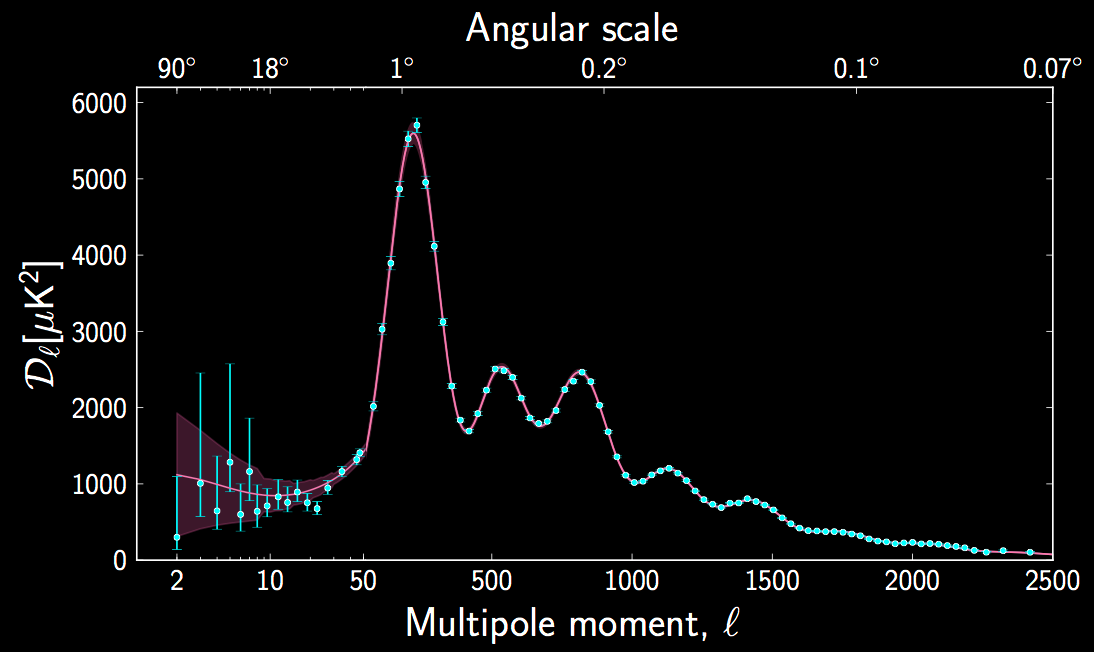
\includegraphics[width=\textwidth]{CUPS/cmb.png}%
        }
        \column{0.45\textwidth}
        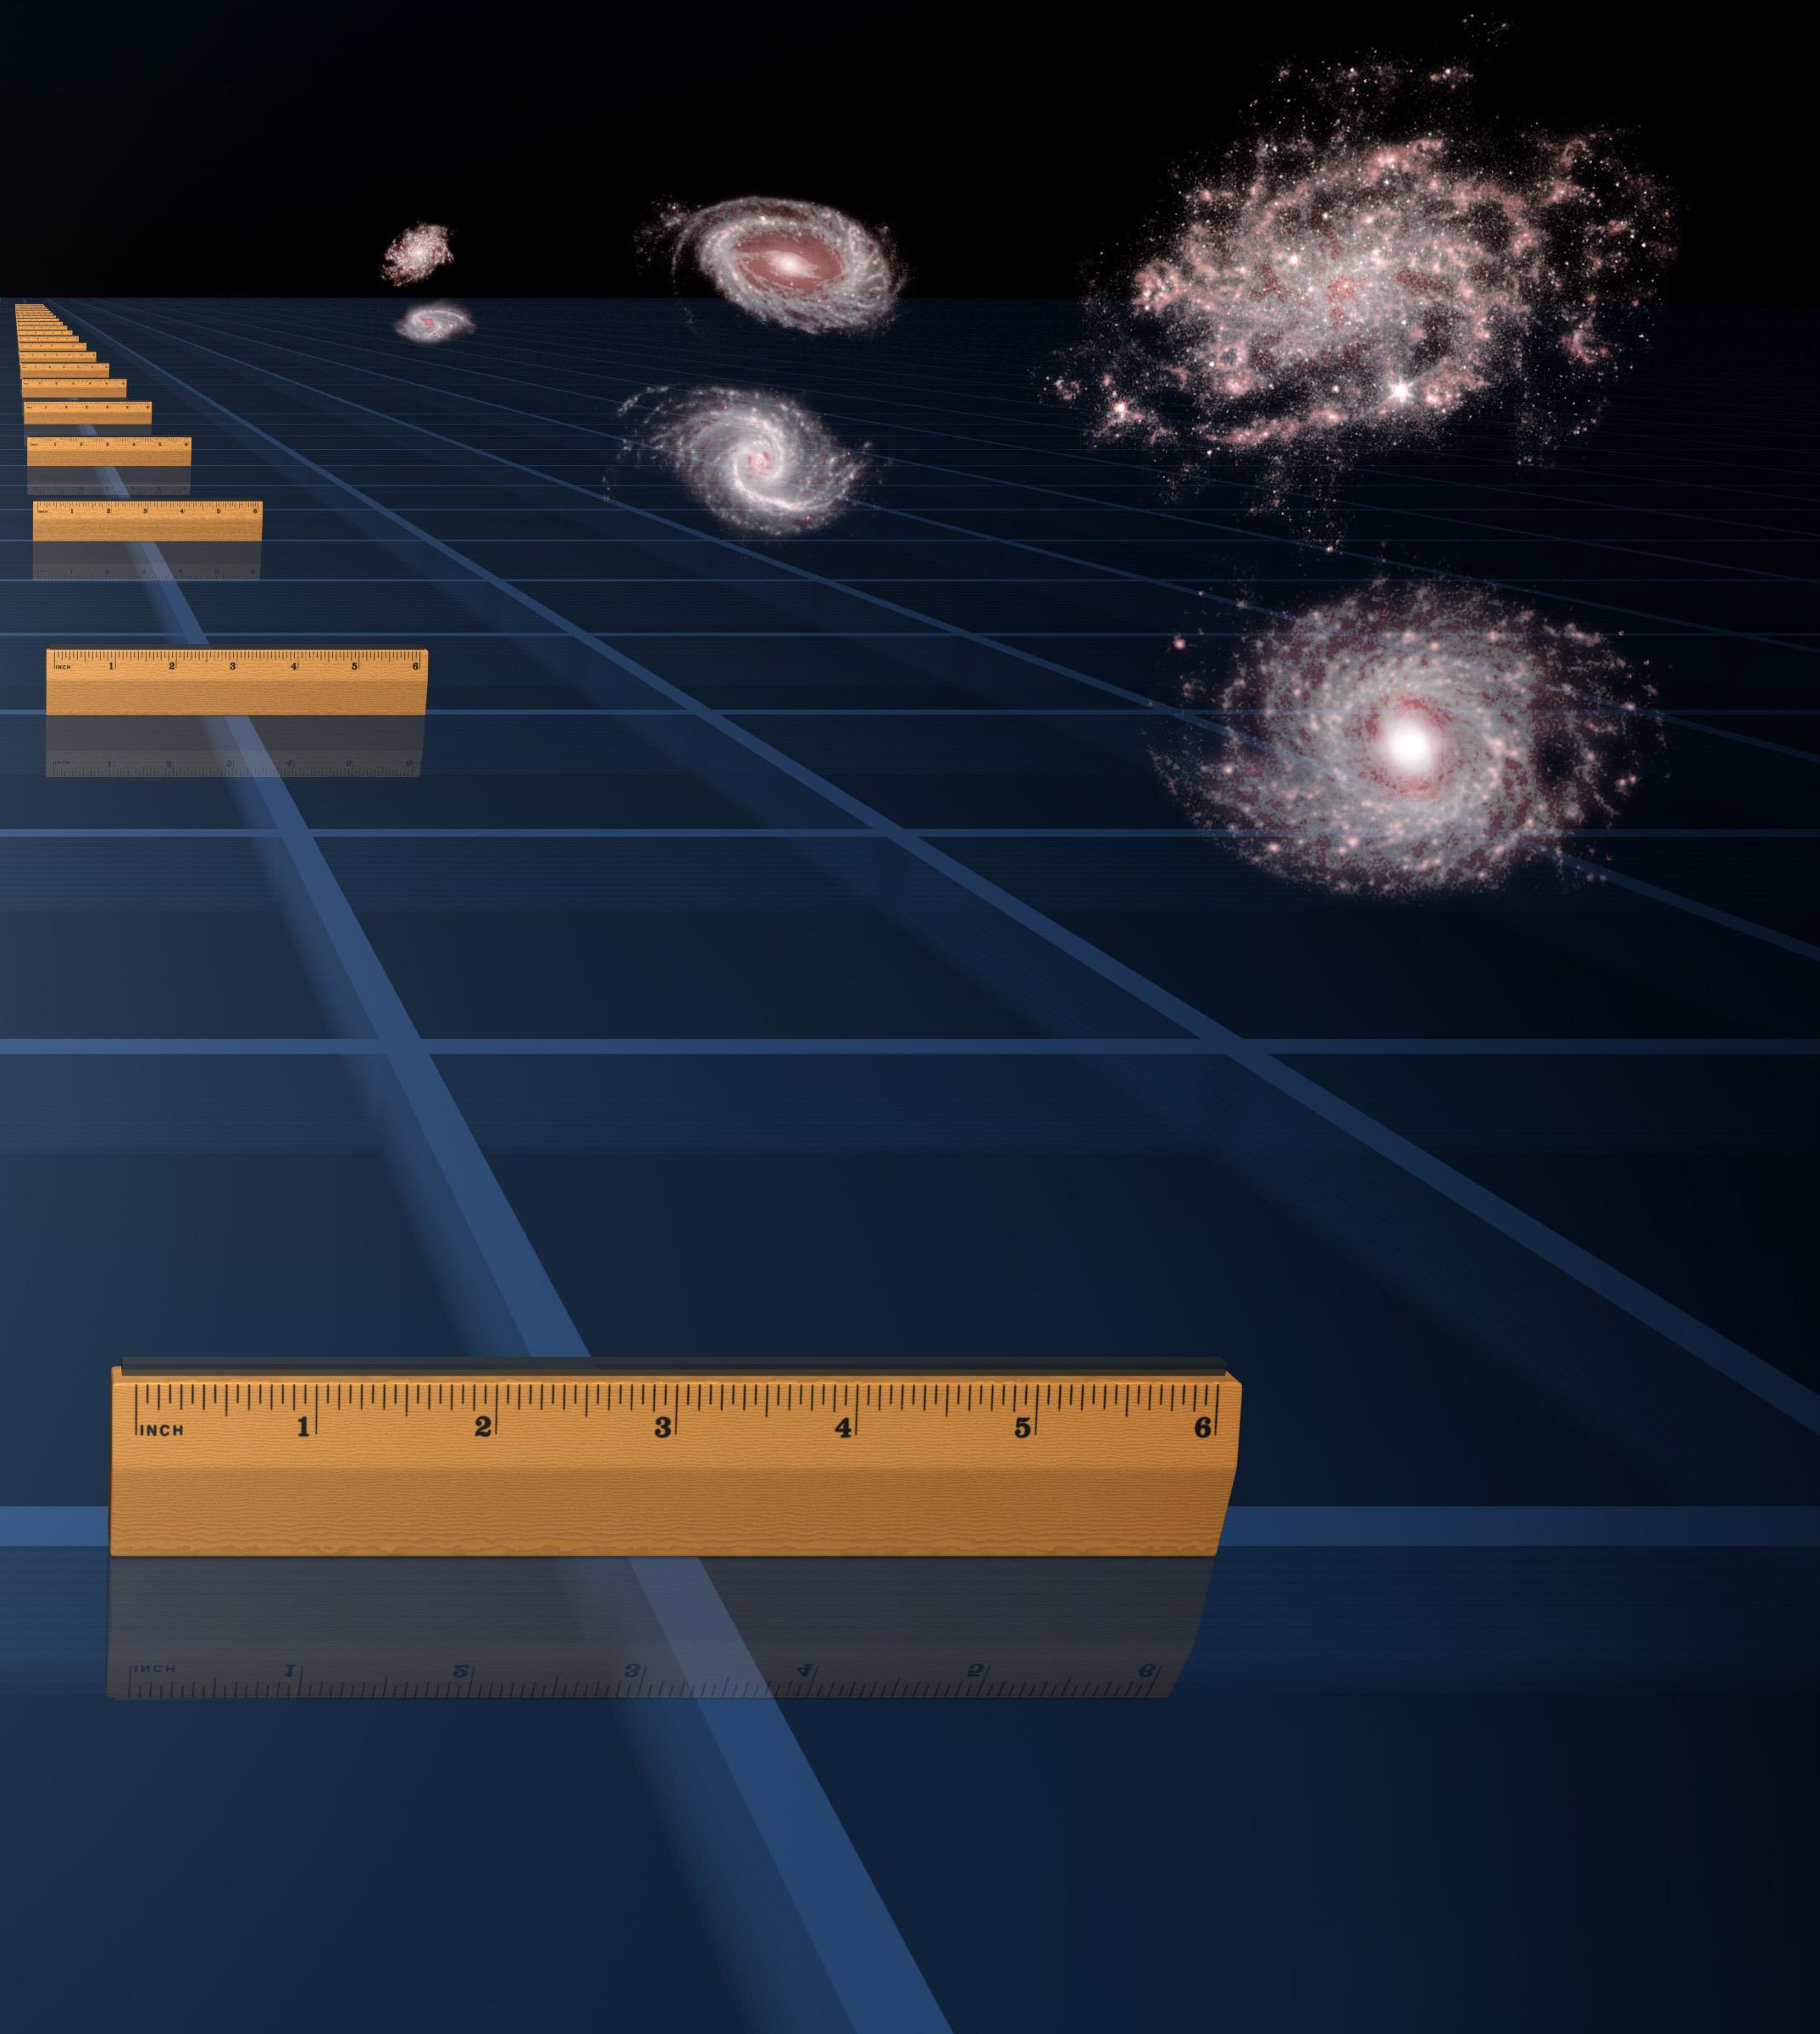
\includegraphics[width=\textwidth]{CUPS/rulers.jpg}
    \end{columns}
\end{frame}

\begin{frame}[label=current]
    \frametitle{Standard sirens}
    \begin{columns}
        \column{0.5\textwidth}
        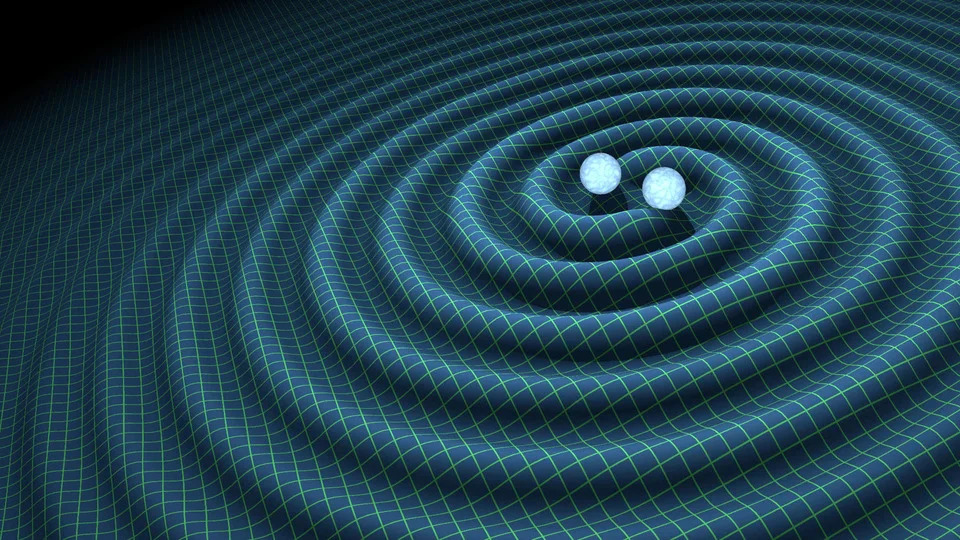
\includegraphics[width=\textwidth]{CUPS/nsns.jpg}
        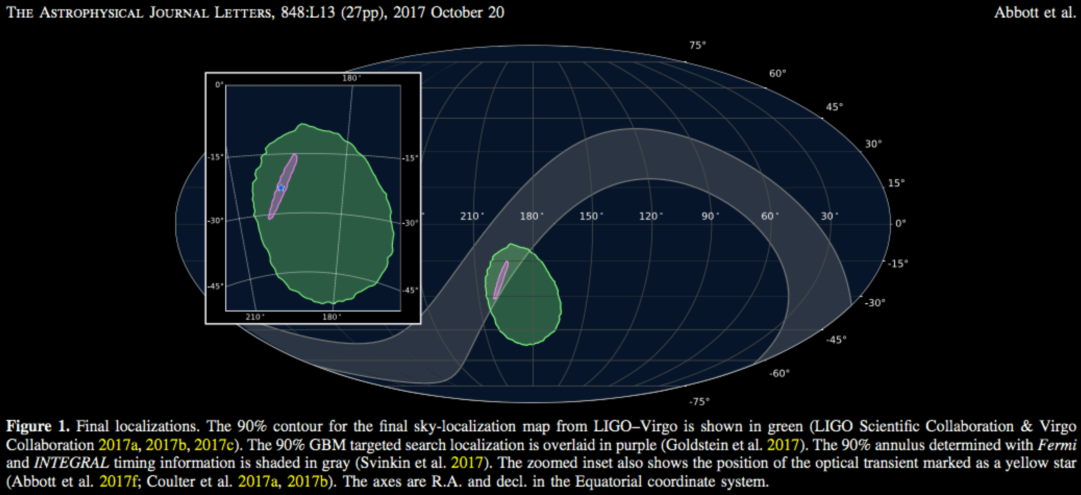
\includegraphics[width=\textwidth]{CUPS/170817location.pdf}
        \column{0.45\textwidth}
        \only<1>{
            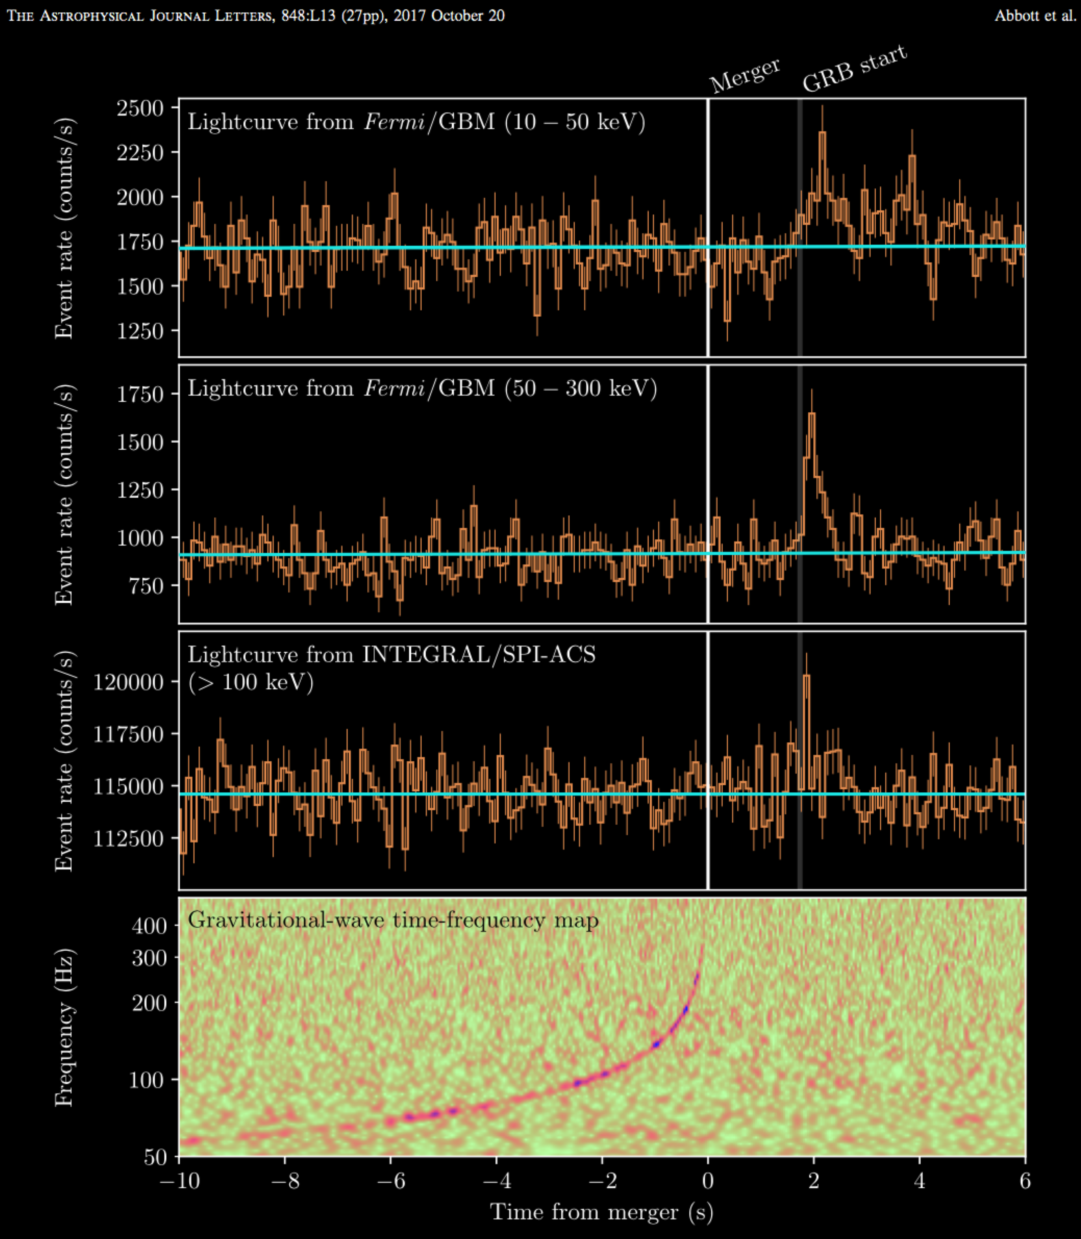
\includegraphics[width=\textwidth]{CUPS/GW170817.pdf}
        }
        \only<2>{
            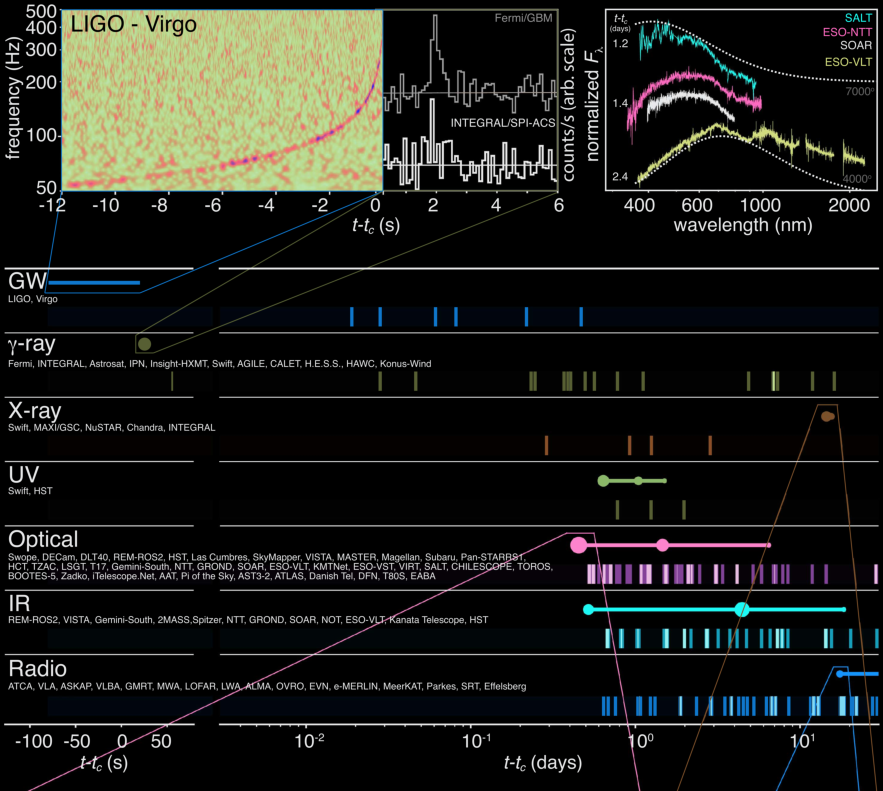
\includegraphics[width=\textwidth]{CUPS/mma_1.pdf}
        }
    \end{columns}
\end{frame}


\begin{frame}[label=current]
    \frametitle{The Hubble tension}
    \begin{columns}
        \column{0.5\textwidth}
            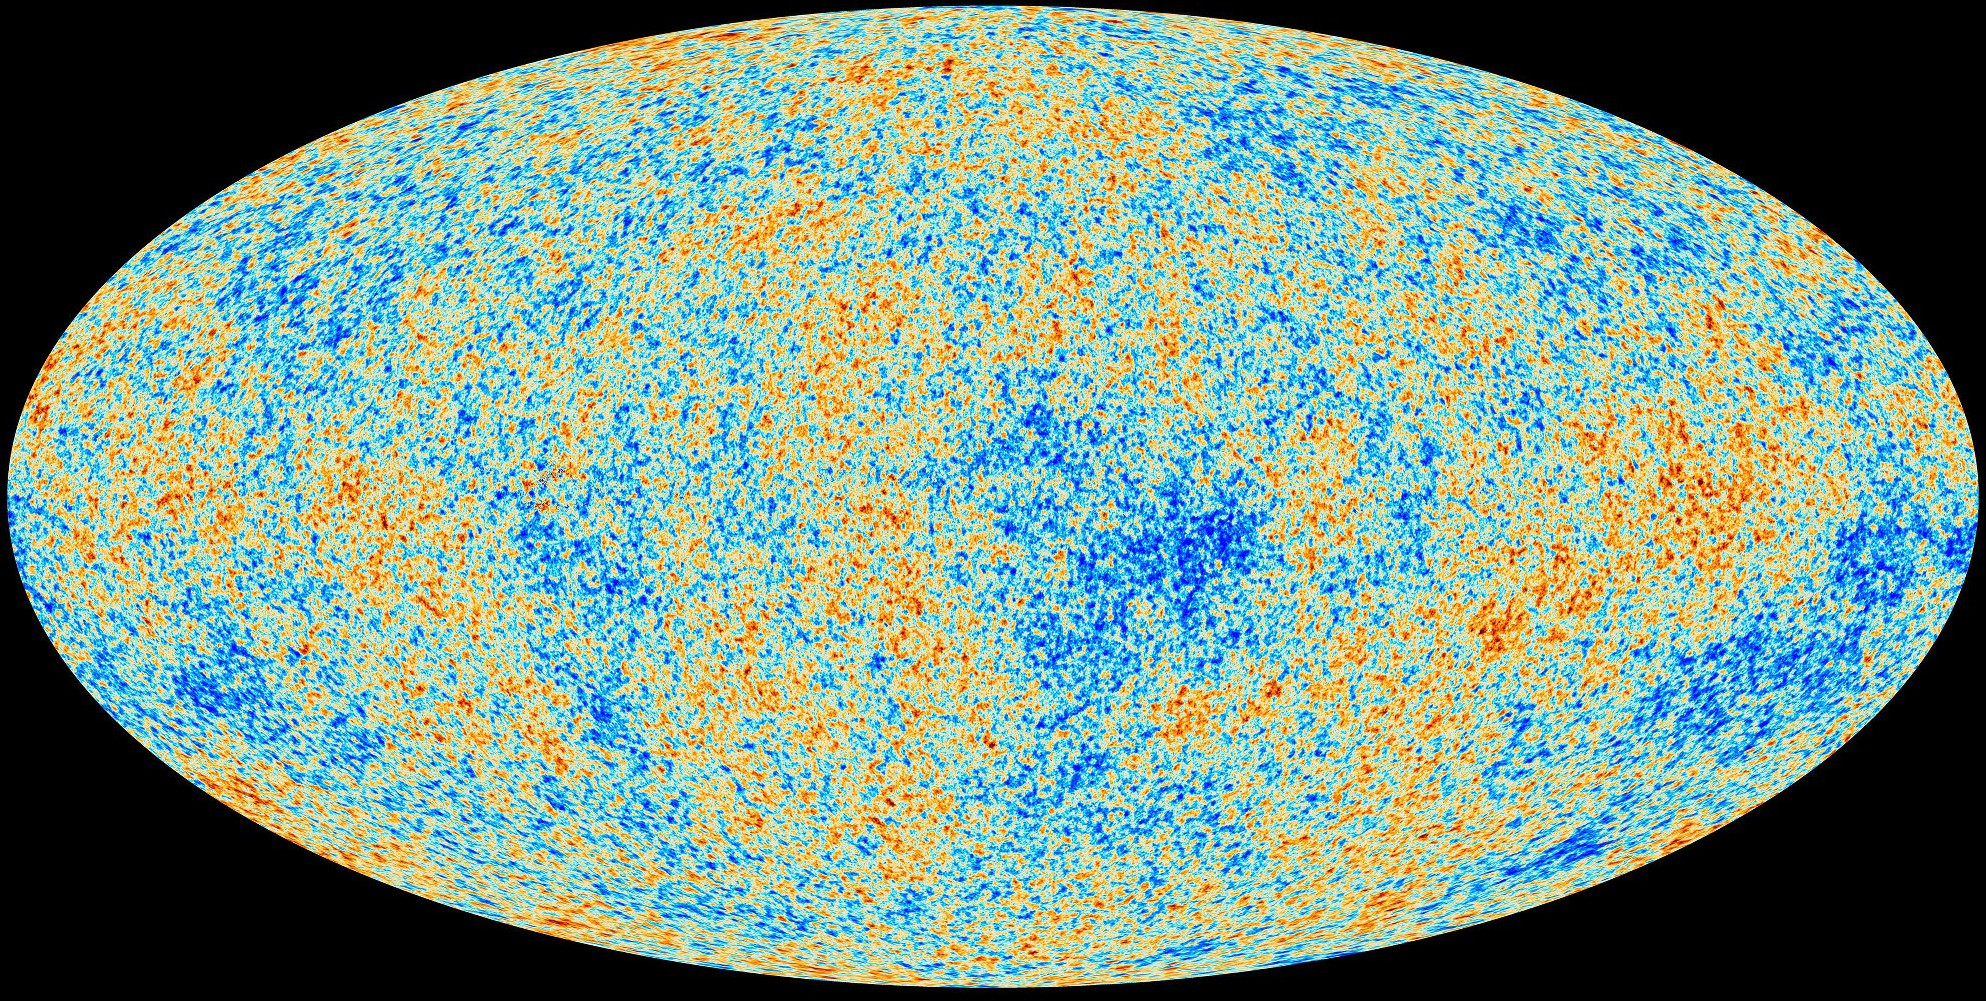
\includegraphics[width=0.5\textwidth]{Images/planckdata}%
            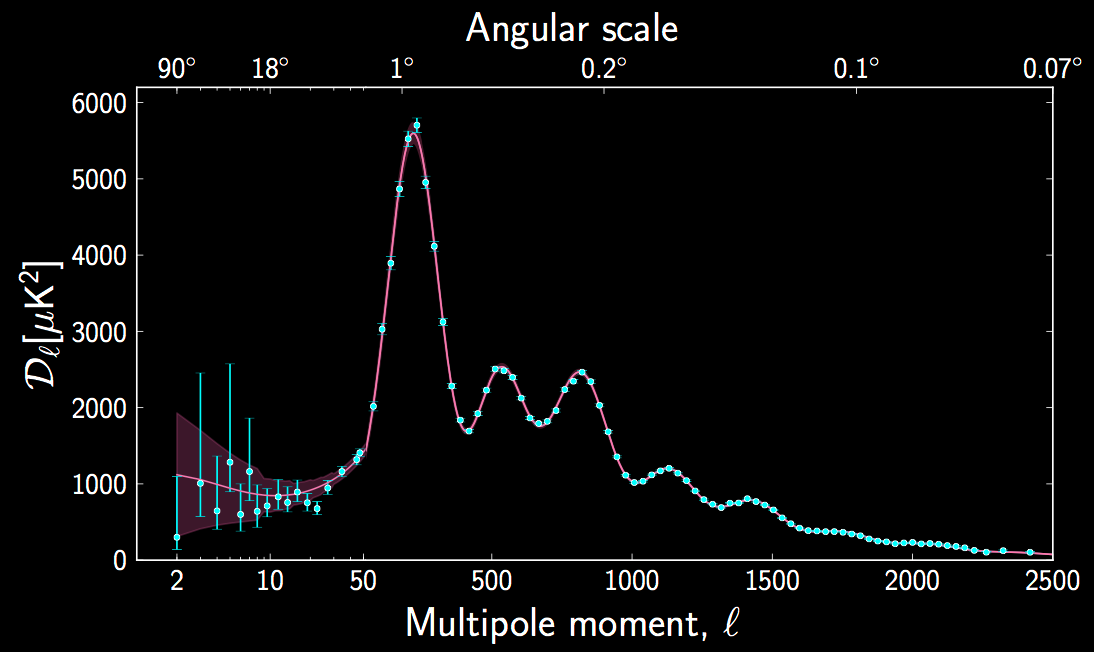
\includegraphics[width=0.49\textwidth]{CUPS/cmb.png}%

            CMB value: $H_0  =67.4 \pm 0.4$
            \pause
            \vspace{10pt}

            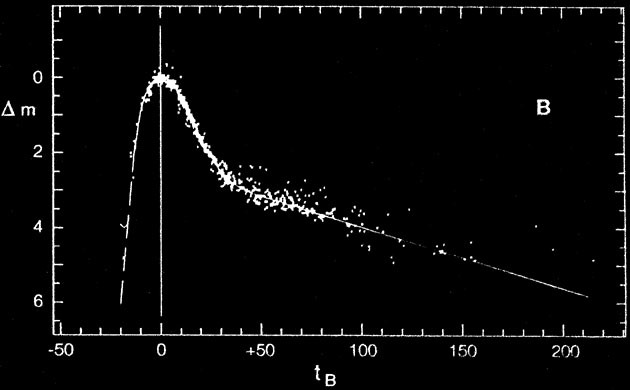
\includegraphics[width=0.49\textwidth]{CUPS/sne.jpeg}
            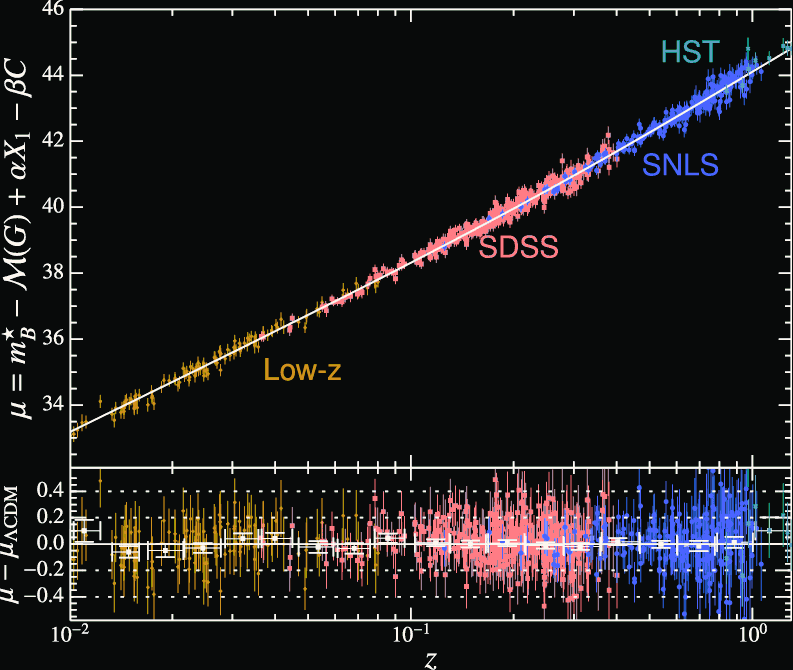
\includegraphics[width=0.49\textwidth]{CUPS/hubble_diagram.png}

            SNe value: $H_0 = 73.0 \pm 1.0$
            \pause
        \column{0.5\textwidth}
        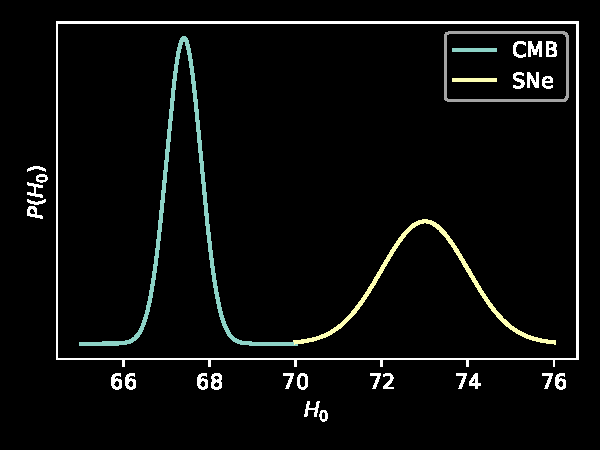
\includegraphics[width=\textwidth]{CUPS/H0.pdf}
    \end{columns}

\end{frame}

\begin{frame}[label=current]
    \frametitle{The Hubble tension}
    \begin{columns}
        \column{0.5\textwidth}
        \begin{itemize}
            \item We call this discrepancy between datasets a ``tension''.
            \item 5.6 km s$^{-1}$ Mpc$^{-1}$ may not seem like much, but this is ``5 sigma''.
            \item If this is real, then something is missing from $\Lambda$CDM.
            \item The last time this happened (90s) we had to invent dark energy!
        %\item SNe is a ``late time'' measurement, whilst CMB is ``early time''
        %\item Something which modifies the physics of only one could explain the difference.
            \item Nobody has (yet) found a convincing solution!
        \end{itemize}
        
        \column{0.5\textwidth}
        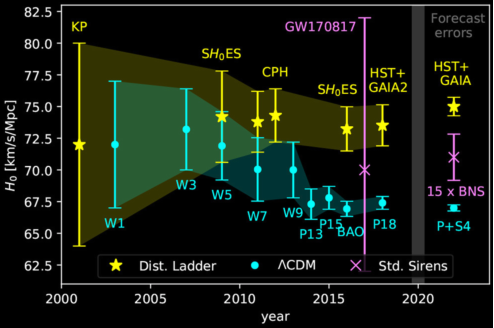
\includegraphics[width=\textwidth]{CUPS/hubble.pdf}
    \end{columns}
\end{frame}


\begin{frame}[label=current]
    \frametitle{Tensions in other parameters}
    \begin{columns}
        \column{0.6\textwidth}
        \begin{itemize}
            \item Famous plot of ``possible universes''
            \item Different values of the (derived) parameters $\Omega_\Lambda$~(dark energy) and $\Omega_M$~(matter)
            \item 2D probability distribution on these parameters
            \item Combined however they give a strong measurement of $\Omega_m\approx0.3$ and $\Omega_\Lambda\approx0.7$, i.e. a flat-$\Lambda$ universe of mostly dark energy today.
            \item<2> Modern measurements less consistent!
            %\item The contours indicate the degree of knowledge provided by CMB (WMAP), Supernovae (SCP) constraints from galaxy clusters (conducted here).
            %\item Note that none of them measure $\Omega_\Lambda$ or $\Omega_m$ directly, and this is characteristic in cosmology.
            %\item Cosmologists therefore need quite a sophisticated understanding of inference to disentangle probability distributions in high-dimensional parameter spaces.
        \end{itemize}
        \column{0.5\textwidth}
        \includegraphics<1>[width=0.8\textwidth]{CUPS/old_parameters.pdf}%
        \includegraphics<2>{CUPS/universe_constraints_zoom.pdf}%
    \end{columns}
\end{frame}

\begin{frame}[label=current]
    \frametitle{Multiparameter tensions}
    \begin{columns}
        \column{0.5\textwidth}
        \begin{itemize}
            \item Picture painted so far is oversimplified.
            \item Cosmological datasets constrain the full 6D parameter space of $\Lambda$CDM.
            \item Triangle plots show this projected into the 1D and 2D subspaces.
            \item Modern Bayesian inference methods capable of manipulating the full ND distribution of a cosmology.
                \[ P(\theta|D,M) = \frac{P(D|\theta,M) P(\theta|M) }{ P(D|M) } \]
            \item Other tensions (e.g. ``Weak lensing'') only show up from the full picture.
        \end{itemize}
        
        \column{0.5\textwidth}
        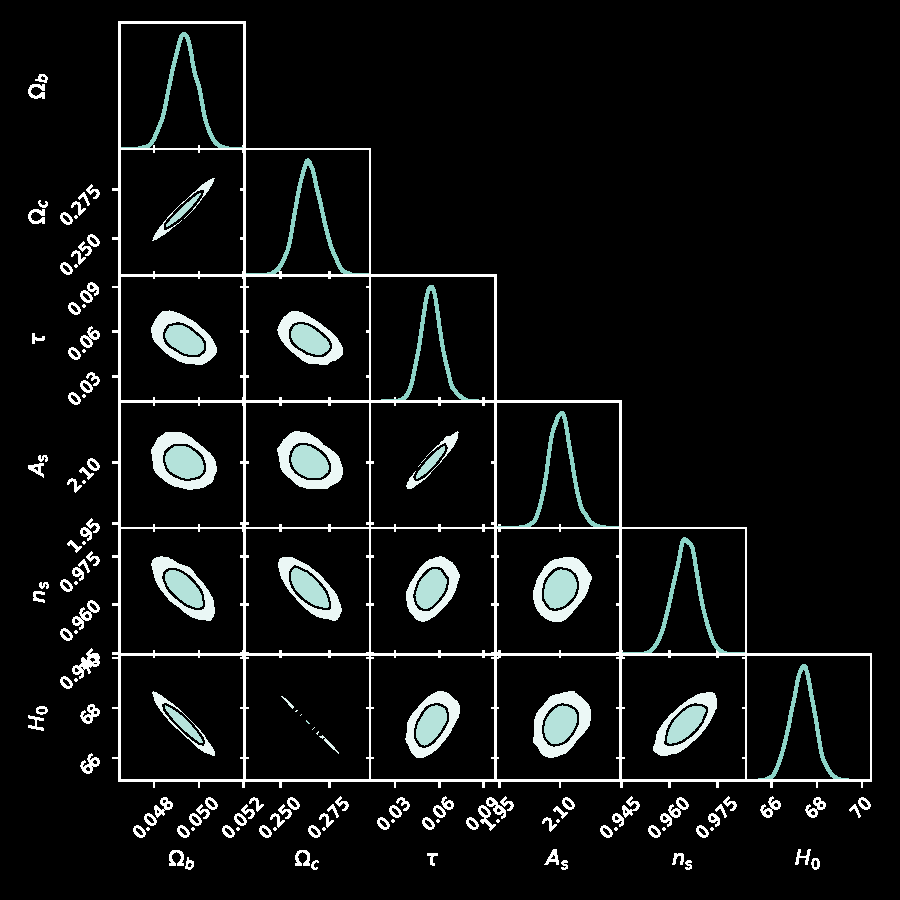
\includegraphics[width=\textwidth]{CUPS/planck_params.pdf}
    \end{columns}
\end{frame}

\begin{frame}[label=current]
    \frametitle{Analysis tensions}
    \begin{itemize}
        \item One of the most common source of tensions is systematic error:
            \begin{description}
                \item[Known knowns:] Current theory
                \item[Known unknowns:] Error/measurement modelling
                \item[Unknown knowns:] New theory!
                \item[Unknown unknowns:] Systematic errors in measurement
            \end{description}
        \item Making combined inferences comes with its own challenges
        \item Sophisticated model comparison is needed to decide which model is ``best''
            \begin{itemize}
                \item Bayes' theorem quantifies Occam's Razor
            \end{itemize}
        \item Next gen instruments likely require machine learning to cope with the data rate
            \begin{itemize}
                \item But these need to be trusted by the scientific community
            \end{itemize}
        \item Cosmology is pushing the frontier of data analysis with simulation-based inference
    \end{itemize}
\end{frame}

\begin{frame}[label=current]
    \frametitle{Theoretical tensions}
    \begin{itemize}
        \item There are long-standing theoretical tensions:
            \begin{enumerate}
                \item Initial conditions: Why is the universe so smooth and flat?
                    \begin{itemize}
                        \item Primordial theories of inflation go some way to explaining this, but some argue these just move the problem back in time
                    \end{itemize}
                \item Entropy tension:
                    \begin{itemize}
                        \item Why did the universe emerge in an anomalously low entropy state?
                    \end{itemize}
                \item Dark tension:
                    \begin{itemize}
                        \item Why do our theories only make sense if the universe is $\approx70\%$ dark energy \\(whose non-zero value is embarrassingly small)?
                        \item Will we ever detect dark matter beyond its gravitational effects?
                    \end{itemize}
                \item Singularity tensions:
                    \begin{itemize}
                        \item We do not have a predictive theory of quantum gravity.
                    \end{itemize}
            \end{enumerate}
        \item Perhaps, like the double slit and photoelectric effect 100 years ago, these observational tensions will lead to a new paradigm shift in physics.
        \item Perhaps we've just got the measurements wrong!
    \end{itemize}
\end{frame}


\begin{frame}[label=current]
    \frametitle{EELT: European Extremely Large Telescope}
    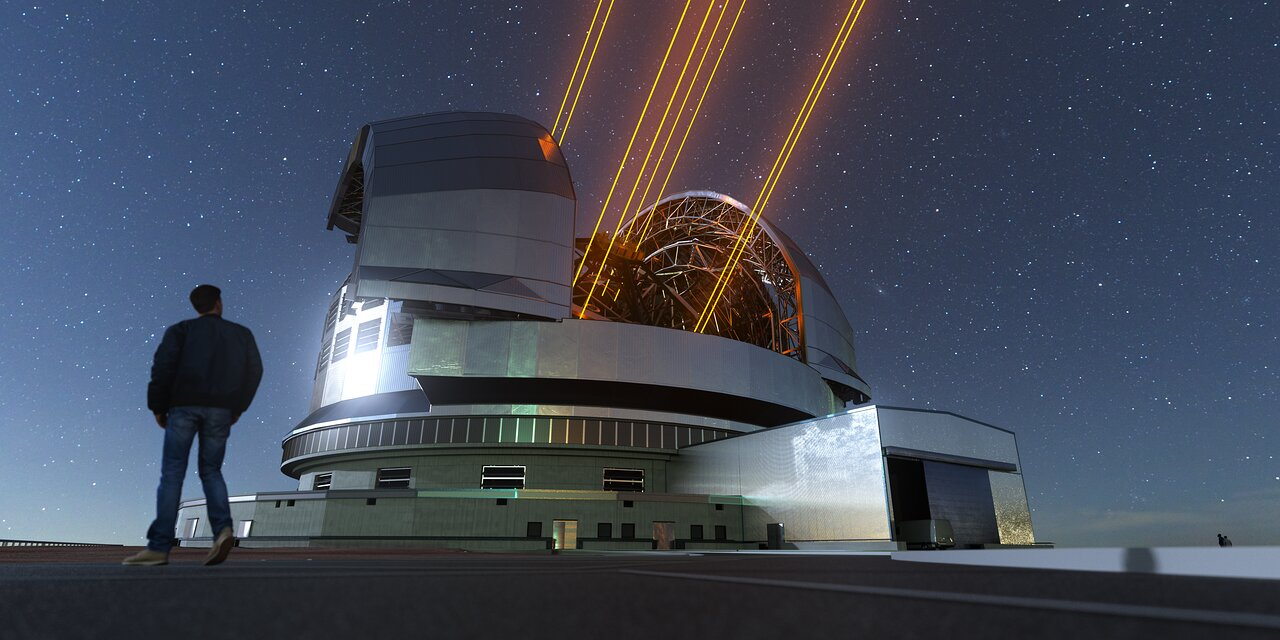
\includegraphics[width=0.5\textwidth]{CUPS/ELT4k-11-Night3_cc.jpg}%
    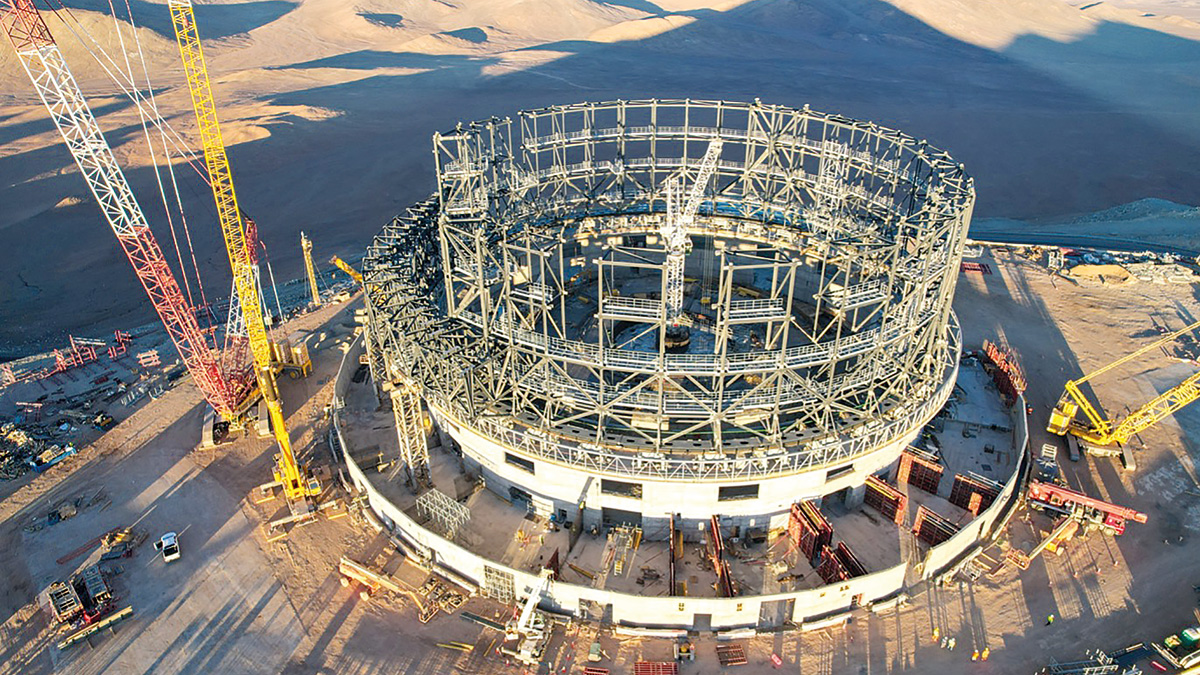
\includegraphics[width=0.5\textwidth]{CUPS/CCSepOct23_NA_ELT.jpg}%
\end{frame}

\begin{frame}[label=current]
    \frametitle{SKA: Square Kilometer Array}
  \centerline{%
      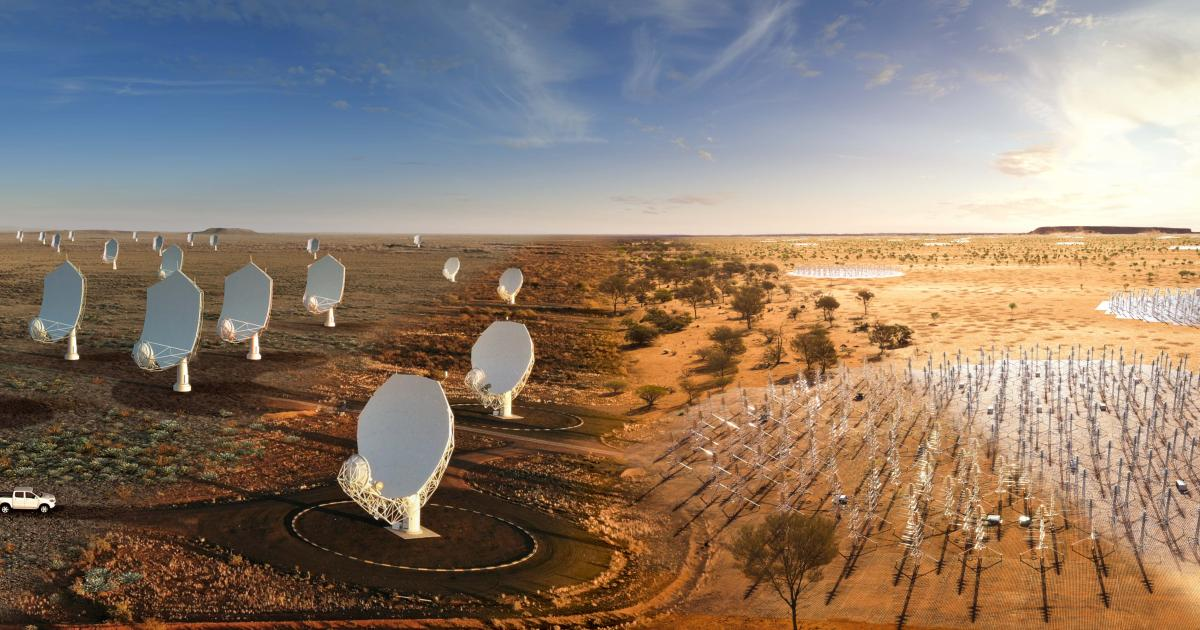
\includegraphics[width=0.5\textwidth]{CUPS/SKA at daytime.jpg}%
      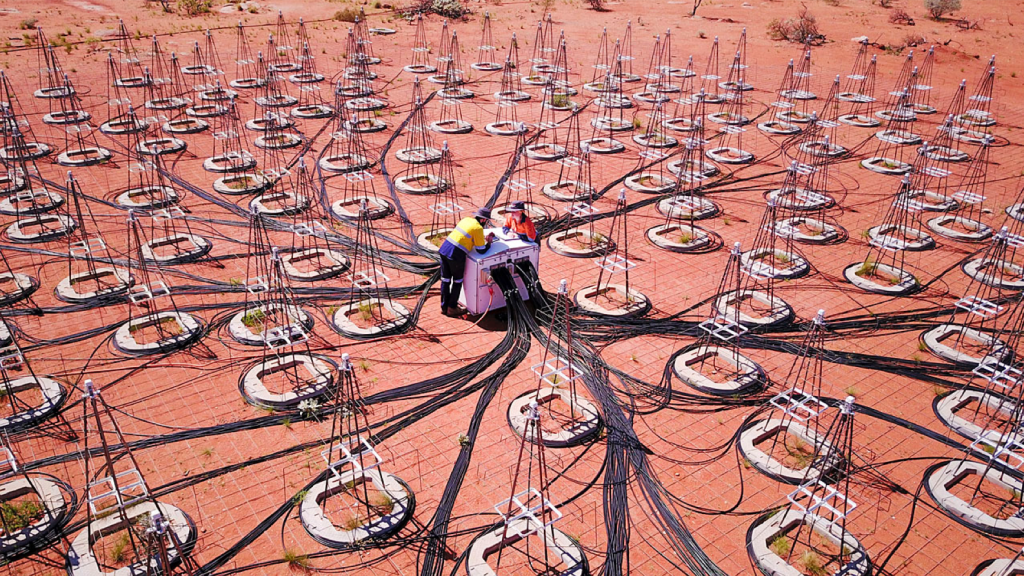
\includegraphics[width=0.5\textwidth]{CUPS/201809_cassiopeia_fig2BryanSKA-1024x576.png }
  }
\end{frame}

\begin{frame}[label=current]
    \frametitle{JWST: James Webb Space Telescope}
  \centerline{%
      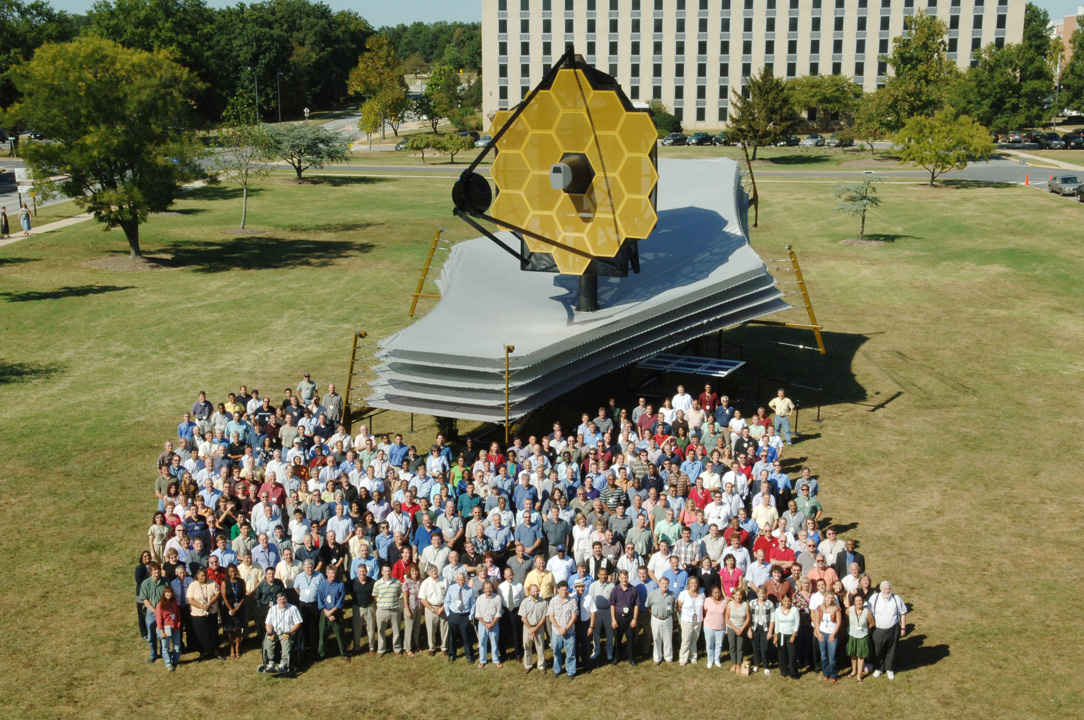
\includegraphics[width=0.8\textwidth]{Images/jwst.jpg}
  }
\end{frame}

\begin{frame}[label=current]
    \frametitle{LIGO/LISA/VIRGO/KAGRA/PTA/Einstein telescopes}
    \begin{columns}
        \column{0.5\textwidth}
        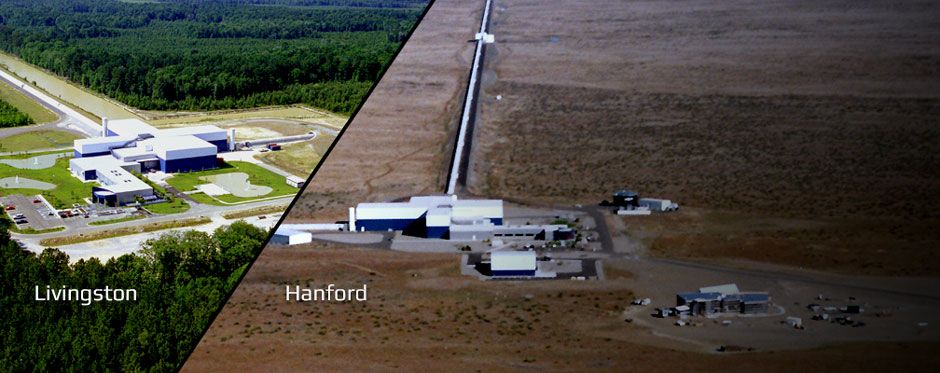
\includegraphics[width=\textwidth]{CUPS/what_slide-ce3596915df0767051e5d7d29c27958a}
        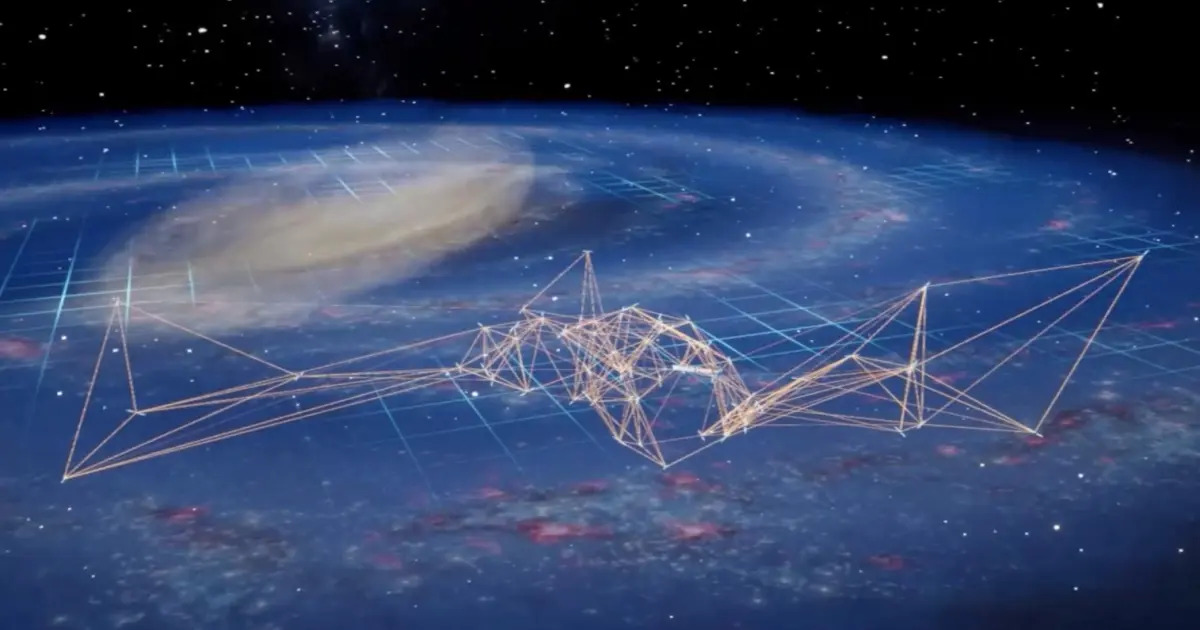
\includegraphics[width=\textwidth]{CUPS/pta.jpg}
        \column{0.5\textwidth}
        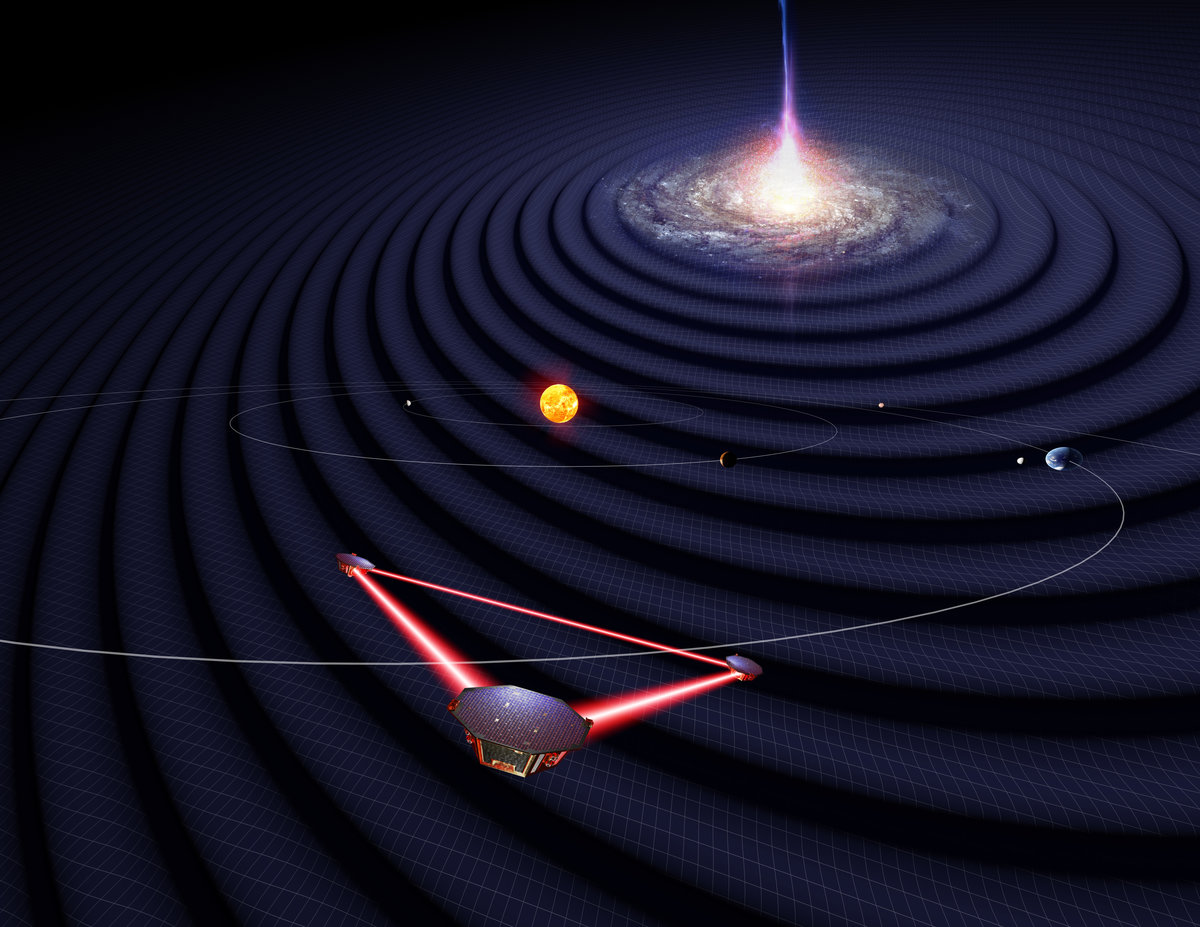
\includegraphics[width=\textwidth]{CUPS/LISA.jpg}
    \end{columns}
\end{frame}

\againframe{why do cosmology}
%\begin{frame}[label=current]
%    \frametitle{Standard sirens}
%    <++>
%\end{frame}

\end{document}
